\documentclass[12pt,a4paper]{article}

% -------------------------------------------------------------------
% PACKAGES
% -------------------------------------------------------------------
\usepackage[spanish]{babel}
\usepackage[utf8]{inputenc}
\usepackage{amsmath}
\usepackage{graphicx}
\usepackage{geometry}
\usepackage{booktabs}
\usepackage{setspace}
\usepackage{hyperref}
\usepackage{float}
\usepackage{tabularx}
\usepackage{graphicx}
\usepackage{subcaption}		
\usepackage{longtable}
\usepackage{multirow}      % (Opcional) Filas combinadas
\usepackage{array}         % Mejoras en tablas
\usepackage{multicol}      % Para entornos de varias columnas


\geometry{margin=2.5cm}
\setstretch{1.15}

\hypersetup{
    colorlinks = true,
    urlcolor = blue,
    linkcolor = black
}

% -------------------------------------------------------------------
% CONFIGURACIÓN GENERAL UTF-8
% -------------------------------------------------------------------

\usepackage[T1]{fontenc}
	

% -------------------------------------------------------------------
% PAQUETES GENERALES
% -------------------------------------------------------------------

\usepackage{xcolor}

\geometry{margin=2.5cm}
\setstretch{1.15}

\hypersetup{
    colorlinks = true,
    urlcolor = blue,
    linkcolor = black
}

% -------------------------------------------------------------------
% LISTINGS (CÓDIGO PYTHON) - CONFIGURACIÓN FULL UTF-8
% -------------------------------------------------------------------
\usepackage{listings}

% Colores para el código
\definecolor{codegray}{rgb}{0.5,0.5,0.5}
\definecolor{codepurple}{rgb}{0.58,0,0.82}
\definecolor{backcolour}{rgb}{0.97,0.97,0.97}

% Soporte de acentos dentro de lstlisting
\lstset{
    literate=
        {á}{{\'a}}1 {é}{{\'e}}1 {í}{{\'i}}1 {ó}{{\'o}}1 {ú}{{\'u}}1
        {Á}{{\'A}}1 {É}{{\'E}}1 {Í}{{\'I}}1 {Ó}{{\'O}}1 {Ú}{{\'U}}1
        {ñ}{{\~n}}1 {Ñ}{{\~N}}1
        {ü}{{\"u}}1 {Ü}{{\"U}}1
        {¿}{{\textquestiondown}}1 
        {¡}{{\textexclamdown}}1
}

% Estilo para Python
\lstdefinestyle{mypython}{
    backgroundcolor=\color{backcolour},
    commentstyle=\color{codegray},
    keywordstyle=\color{blue},
    numberstyle=\tiny\color{codegray},
    stringstyle=\color{codepurple},
    basicstyle=\ttfamily\footnotesize,
    breaklines=true,
    numbers=left,
    numbersep=5pt,
    frame=single,
    tabsize=4
}

% -------------------------------------------------------------------
% DOCUMENT
% -------------------------------------------------------------------
\begin{document}

% -------------------------------------------------------------------
% PORTADA
% -------------------------------------------------------------------
\begin{titlepage}
    \centering

    % LOGO UIB (posa el logo al mateix directori del .tex)
    
\includegraphics[width=4cm]{uib_logo.png}\par
    \vspace{0.5cm}

    {\Large Universitat de les Illes Balears \par}
    {\large Grau en Enginyeria Informàtica \par}

    \vfill

    {\Huge \bfseries Pràctica d'Aprenentatge Automàtic\par}
    \vspace{0.4cm}
    {\Large NODE21: Classificació de Radiografies de Pit\par}
    \vspace{0.2cm}
    {\large \textit{Detecció de nòduls pulmonars en imatges CXR}\par}

    \vfill
    % Autors
    {\large \textbf{Autors:}\par}
    {\large Toni Contesti \par}
    {\large Marc Link Cladera \par}
    \vspace{0.5cm}

    % Professor
    {\large \textbf{Professor:} Miquel Miró Nicolau\par}

    \vfill
    {\large Curs 2025--2026\par}
\end{titlepage}


\tableofcontents
\newpage

\section{Introducció}

L’ús de l’aprenentatge automàtic en l’anàlisi d’imatges mèdiques ha experimentat un creixement notable durant la darrera dècada. Les radiografies de tòrax (CXR) constitueixen una de les proves diagnòstiques més utilitzades a l’àmbit clínic, però també una de les més difícils d’interpretar. La superposició d’estructures anatòmiques, la presència de soroll i la variabilitat d’adquisició fan que lesions petites com els nòduls pulmonars siguin sovint subtils o fins i tot invisibles per al diagnòstic humà.

El repte NODE21 \cite{nia2025} --- descrit a l’enunciat oficial de la pràctica (pàgines I–III) \cite{uiaa2025} --- proposa precisament abordar aquests reptes mitjançant tècniques modernes d’intel·ligència artificial. Les dades consisteixen en radiografies de pit en format \texttt{.mha}, i el repte es divideix en tres àrees principals:
\begin{enumerate}
    \item \textbf{Classificació binària}: determinar si una imatge conté almenys un nòdul pulmonar.
    \item \textbf{Detecció}: predir la posició exacta dels nòduls mitjançant bounding boxes.
    \item \textbf{Generació}: crear nòduls sintètics per millorar els models anteriors.
\end{enumerate}

En el marc d’aquesta pràctica ens centrarem en les dues primeres, que també són les que apareixen com a tasques avaluables a l’enunciat oficial. L’objectiu global del treball és, per tant, desenvolupar un sistema complet capaç de:
\begin{itemize}
    \item classificar radiografies com a \textit{positives} o \textit{negatives} per presència de nòduls;
    \item detectar la localització aproximada del nòdul dins la imatge.
\end{itemize}

\subsection{Estructura del document}

Aquesta memòria s’organitza en dues parts principals, seguint l’ordre natural del desenvolupament del projecte:

\begin{description}
    \item[\textbf{Primera part: Classificació binària}]  
    Descrivim tot el procés dut a terme per construir un model de classificació robust: preprocessament intensiu, generació de canals addicionals (CLAHE, contorns, FFT, Homomorphic Filtering, LoG, Band-Pass), equilibratge del dataset, proves amb models clàssics (KNN, SVM, regressió logística, Random Forest), models de deep learning i adaptació d’EfficientNet a entrades multicanal.

    \item[\textbf{Segona part: Detecció i segmentació morfològica}]  
    En aquesta part abordem la detecció de nòduls utilitzant bounding boxes i tècniques complementàries de realçament i “pseudosegmentació” (mapes de contorn, LoG multi-escala, filtres banda-pas orientats a la mida del nòdul). Si bé no es realitza segmentació pixel-a-pixel, incloem diverses aproximacions basades en transformades freqüencials i espai-freqüència que permeten identificar i delimitar la regió nodular amb més precisió.
\end{description}

\subsection{Enfocament general}

El treball segueix una metodologia iterativa que combina tècniques clàssiques i profundes:
\begin{enumerate}
    \item Exploració del dataset NODE21 i lectura d’imatges \texttt{.mha}.
    \item Correcció d’orientació i normalització.
    \item Preprocessament multicanal i millores innovadores.
    \item Entrenament i comparació de models de classificació.
    \item Visualització, localització i detecció aproximada dels nòduls.
    \item Avaluació mitjançant mètriques estàndard (Accuracy, F1-score, IoU).
\end{enumerate}

Aquesta estructura reflecteix fidelment el progrés real del projecte, des dels primers intents de classificació fins a l’experimentació amb tècniques més avançades orientades a la detecció i segmentació.


	
\section{Preparació i gestió del dataset NODE21}

Per poder treballar amb el conjunt de dades NODE21, proporcionat en format \texttt{.mha}, ha estat necessari habilitar un entorn de treball que permetés tant la càrrega eficient de les imatges com la seva exploració inicial. En aquesta pràctica s’ha utilitzat \textbf{Google Colab} com a plataforma principal d’execució, ja que proporciona GPU, accés a llibreries científiques i integració directa amb Google Drive.

\subsection{Configuració inicial de l’entorn}

El primer pas ha estat instal·lar la llibreria \texttt{OpenCXR}, necessària per llegir imatges mèdiques en format \texttt{.mha}, tal com recomana l’enunciat de la pràctica (pàg. II) \cite{uiaa2025}. La instal·lació es realitza amb:

\begin{lstlisting}[style=mypython]
!pip install opencxr
\end{lstlisting}

A continuació s’ha muntat Google Drive per accedir als fitxers emmagatzemats. Aquesta acció és imprescindible, ja que les imatges del repte NODE21 es troben en un directori dins del nostre Drive:

\begin{lstlisting}[style=mypython]
from google.colab import drive
drive.mount('/content/drive')
\end{lstlisting}

Un cop muntat, s’han creat rutes de treball clares per accedir a les imatges i al fitxer \texttt{metadata.csv}:

\begin{lstlisting}[style=mypython]
BASE_PATH = "/content/drive/MyDrive/ML/DATASETS/NODE21/proccessed_data"
PATH_IMAGES = f"{BASE_PATH}/images"
PATH_METADATA = f"{BASE_PATH}/metadata.csv"
\end{lstlisting}

\subsection{Càrrega i inspecció del fitxer de metadades}

El fitxer \texttt{metadata.csv} conté informació essencial per a cada imatge, com ara:

\begin{itemize}
    \item el nom del fitxer (\texttt{img\_name});
    \item l’etiqueta de classificació (\texttt{label});
    \item coordenades del nòdul (\texttt{x}, \texttt{y}, \texttt{width}, \texttt{height}).
\end{itemize}

La càrrega es realitza amb:

\begin{lstlisting}[style=mypython]
import pandas as pd
import os

df = pd.read_csv(PATH_METADATA)
df.head()
\end{lstlisting}

S’ha afegit la ruta completa de cada imatge al DataFrame:

\begin{lstlisting}[style=mypython]
df["file_path"] = df["img_name"].apply(
    lambda x: os.path.join(PATH_IMAGES, x)
)
\end{lstlisting}

\subsection{Validació d’arxius i detecció d’imatges inexistents}

Abans d'entrenar models, és essencial verificar quines rutes no existeixen físicament al disc:

\begin{lstlisting}[style=mypython]
missing = df[~df["file_path"].apply(os.path.exists)]
print("Imatges que falten:", len(missing))
missing.head()
\end{lstlisting}

Aquest pas evita errors durant l'entrenament, ja que NODE21 pot contenir imatges absents o corruptes.

\subsection{Visualització inicial de les imatges .mha}

S’ha carregat una imatge d’exemple per validar la lectura amb OpenCXR:

\begin{lstlisting}[style=mypython]
from opencxr.utils.file_io import read_file
import matplotlib.pyplot as plt

sample_path = df["file_path"].iloc[1001]
img_np, spacing, _ = read_file(sample_path)

plt.imshow(img_np, cmap="gray")
plt.title("Imatge de mostra")
plt.axis("on")
plt.show()
\end{lstlisting}

Aquesta inspecció visual ha confirmat:

\begin{itemize}
    \item orientació inconsistent en les imatges,
    \item variacions en el rang d'intensitats,
    \item resolucions no uniformes.
\end{itemize}

Com a conseqüència d’aquestes observacions inicials, una de les primeres tasques ha estat
estandarditzar l’orientació de totes les imatges del conjunt NODE21. Durant l’exploració
visual es va comprovar que les imatges es trobaven:

\begin{itemize}
    \item invertides horitzontalment (l’hemidíafragma dret apareixia a l’esquerra),
    \item i rotades 90 graus en sentit antihorari.
\end{itemize}

Per tal de garantir una coherència anatòmica en totes les radiografies i evitar errors en les
etapes de preprocessament i entrenament, es va aplicar una correcció d’orientació homogènia
a totes les imatges abans de qualsevol altre pas del pipeline.

La correcció aplicada consisteix en:

\begin{enumerate}
    \item una rotació de \(90^\circ\) cap a la dreta (\(\texttt{k=3}\) en \texttt{numpy.rot90}),
    \item seguida d’una inversió horitzontal mitjançant \texttt{numpy.fliplr}.
\end{enumerate}

Aquest procediment reordena totes les imatges de manera consistent, situant els pulmons en
la seva orientació anatòmica habitual (pulmó dret a la dreta de la imatge i cor lleugerament
desplaçat cap a l’esquerra). A partir d’aquest punt, tot el processament posterior —normalització,
reescalat, generació de canals addicionals i entrenament dels models— es realitza sobre dades
corretament orientades.


\subsection{Creació d’un Dataset personalitzat}

Per entrenar models amb PyTorch, s’ha encapsulat la lògica de lectura i preprocessament en una classe:

\begin{lstlisting}[style=mypython]
import cv2
from torch.utils.data import Dataset
import torch
import numpy as np
import os

class CXRClassificationDataset(Dataset):
    def __init__(self, df):
        self.df = df[df["file_path"].apply(os.path.exists)].reset_index(drop=True)

    def __len__(self):
        return len(self.df)

    def __getitem__(self, idx):
        row = self.df.iloc[idx]
        img_path = row["file_path"]

        if not os.path.exists(img_path):
            return {"error": True}

        img_np, _, _ = read_file(img_path)

        img = img_np.astype(np.float32)
        img = (img - img.min()) / (img.max() - img.min())

        img = cv2.resize(img, (224,224))
        img = np.expand_dims(img, axis=0)

        return {
            "error": False,
            "image": torch.tensor(img, dtype=torch.float32),
            "label": torch.tensor(row["label"], dtype=torch.long)
        }

def custom_collate(batch):
    batch = [item for item in batch if item is not None and not item.get("error", False)]
    if len(batch) == 0:
        return None

    images = torch.stack([item["image"] for item in batch])
    labels = torch.stack([item["label"] for item in batch])
    return images, labels
\end{lstlisting}

\subsection{Resum dels passos realitzats}

\begin{enumerate}
    \item Instal·lació d’OpenCXR.
    \item Muntatge de Google Drive.
    \item Definició de rutes i càrrega de metadades.
    \item Afegir la ruta completa de cada imatge.
    \item Detecció d’imatges inexistents.
    \item Visualització preliminar.
    \item Implementació d’un Dataset PyTorch robust.
\end{enumerate}

Aquest flux estableix el fonament per al preprocessament, l’augment de dades i els models de classificació i detecció desenvolupats en les seccions següents.

\section{Model 1: Classificació amb una CNN Simple Entrenada Des de Zero}

Com a primer experiment del projecte, i seguint estrictament l’enunciat de la
pràctica, es va implementar una xarxa neuronal convolucional (\textit{CNN}) construïda
completament des de zero, sense recórrer a arquitectures preentrenades. Aquest model
serveix com a \textbf{baseline} per quantificar les millores que aportaran posteriorment
el processament multicanal, el reequilibrat del dataset i l’ús d’EfficientNet.

\subsection{Arquitectura del Model}

L’arquitectura emprada és una CNN clàssica composta per tres blocs
convolucionals amb activació ReLU i operacions de max-pooling, seguits d’un
classificador dens. Aquesta estructura permet extreure progressivament característiques
de nivell superior, tot i que la seva capacitat representacional és limitada en
comparació amb models moderns.

\begin{itemize}
    \item \textbf{Blocs convolucionals}:
    \begin{itemize}
        \item Conv2D $(1 \rightarrow 16)$ + ReLU + MaxPool
        \item Conv2D $(16 \rightarrow 32)$ + ReLU + MaxPool
        \item Conv2D $(32 \rightarrow 64)$ + ReLU + MaxPool
    \end{itemize}

    \item \textbf{Classificador final}:
    \begin{itemize}
        \item Flatten
        \item Linear $(64 \cdot 28 \cdot 28 \rightarrow 128)$ + ReLU + Dropout(0.3)
        \item Linear $(128 \rightarrow 2)$ per a classificació binària
    \end{itemize}
\end{itemize}

La implementació en PyTorch es detalla en el fragment següent:

\begin{lstlisting}[style=mypython]
class SimpleCNN(nn.Module):
    def __init__(self):
        super(SimpleCNN, self).__init__()

        # Blocs convolucionals
        self.conv_layers = nn.Sequential(
            nn.Conv2d(1, 16, kernel_size=3, padding=1),
            nn.ReLU(),
            nn.MaxPool2d(2),

            nn.Conv2d(16, 32, kernel_size=3, padding=1),
            nn.ReLU(),
            nn.MaxPool2d(2),

            nn.Conv2d(32, 64, kernel_size=3, padding=1),
            nn.ReLU(),
            nn.MaxPool2d(2),
        )

        # Classificador
        self.fc_layers = nn.Sequential(
            nn.Flatten(),
            nn.Linear(64 * 28 * 28, 128),
            nn.ReLU(),
            nn.Dropout(0.3),
            nn.Linear(128, 2)
        )

    def forward(self, x):
        x = self.conv_layers(x)
        x = self.fc_layers(x)
        return x
\end{lstlisting}

Aquest model accepta imatges de mida $224 \times 224$ i un sol canal, utilitzant la
imatge normalitzada sense cap processament addicional.

\subsection{Preparació del Conjunt de Dades}

El dataset NODE21 es va dividir en un 80\% per a entrenament i un 20\% per a test mitjançant
\texttt{train\_test\_split}. El \textit{Dataset} personalitzat utilitzat en seccions
prèvies inclou la normalització d’intensitats i el reescalat de totes les imatges a la
mida requerida per la CNN.

\[
\text{Mida entrenament: } 4179, \qquad
\text{Mida test: } 1045.
\]

A més, es va emprar un \texttt{custom\_collate} per descartar imatges absents detectades
durant la validació del dataset.

\subsection{Configuració de l’Entrenament}

L’entrenament es va realitzar durant 10 èpoques consecutives amb la configuració següent:

\begin{itemize}
    \item Optimitzador: \textbf{Adam}
    \item Learning rate: $1 \times 10^{-3}$
    \item Funció de pèrdua: \textbf{CrossEntropyLoss}
    \item Batch size: 16
    \item Entrenament accelerat en GPU quan estava disponible
\end{itemize}

El bucle d’entrenament va incloure el càlcul de la pèrdua, l’exactitud i el registre dels
valors per època per a la seva anàlisi posterior.

\subsection{Codi del Procés d’Entrenament}

\begin{lstlisting}[style=mypython]
criterion = nn.CrossEntropyLoss()
optimizer = optim.Adam(model.parameters(), lr=1e-3)

epochs = 10
train_losses = []
train_accs = []

for epoch in range(epochs):
    model.train()
    running_loss = 0
    correct = 0
    total = 0

    for images, labels in train_loader:
        images, labels = images.to(device), labels.to(device)

        optimizer.zero_grad()
        outputs = model(images)
        loss = criterion(outputs, labels)
        loss.backward()
        optimizer.step()

        running_loss += loss.item()
        _, predicted = torch.max(outputs, 1)
        total += labels.size(0)
        correct += (predicted == labels).sum().item()

    epoch_loss = running_loss / len(train_loader)
    epoch_acc = correct / total
\end{lstlisting}

\subsection{Resultats de l’Entrenament}

La Taula~\ref{tab:simplecnn_epochs} mostra els valors reals de pèrdua i exactitud
obtinguts en cadascuna de les deu èpoques.

\begin{table}[h!]
\centering
\begin{tabular}{c|c|c}
\hline
\textbf{Època} & \textbf{Pèrdua} & \textbf{Accuracy} \\
\hline
1  & 0.5966 & 0.7169 \\
2  & 0.5316 & 0.7222 \\
3  & 0.5036 & 0.7284 \\
4  & 0.4931 & 0.7365 \\
5  & 0.4757 & 0.7504 \\
6  & 0.4695 & 0.7631 \\
7  & 0.4497 & 0.7724 \\
8  & 0.4222 & 0.8007 \\
9  & 0.4001 & 0.8069 \\
10 & 0.3750 & 0.8227 \\
\hline
\end{tabular}
\caption{Evolució de la pèrdua i de l’exactitud durant l’entrenament de la CNN simple.}
\label{tab:simplecnn_epochs}
\end{table}

El comportament observat és raonable: pèrdua decreixent i millora contínua de
l’exactitud, assolint un 82.27\% al final de l’entrenament. Tanmateix, s’observen indicis
de sobreajust a partir de les èpoques 7--8.

La Figura~\ref{fig:simplecnn_training} mostra les corbes de pèrdua i exactitud al llarg de
les 10 èpoques d’entrenament. S’observa una disminució progressiva de la pèrdua i un
augment estable del rendiment, assolint valors superiors al 80\% en les darreres
èpoques. Aquest comportament és coherent amb un model entrenat des de zero i amb una
capacitat limitada, que aprèn de manera gradual però consistent.

\begin{figure}[H]
    \centering
    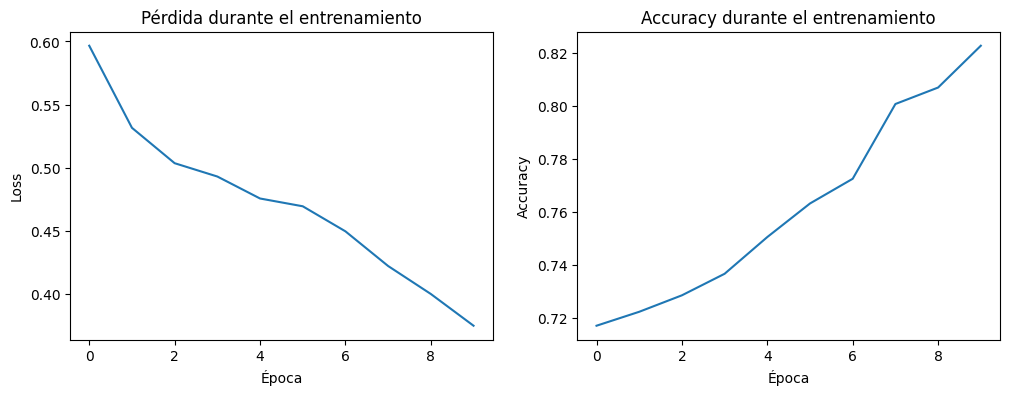
\includegraphics[width=0.95\textwidth]{images/perdida_accuracy_entrenamiento_cnn.png}
    \caption{Evolució de la pèrdua (esquerra) i de l’exactitud (dreta) del model SimpleCNN durant l’entrenament.}
    \label{fig:simplecnn_training}
\end{figure}

\subsection{Avaluació del Model sobre el Conjunt de Test}

L’avaluació es va realitzar sobre el 20\% reservat del dataset (1045 mostres). El model
va obtenir una exactitud final de:

\[
\text{Accuracy}_{\text{test}} = 0.7904
\]

Aquest valor confirma que, tot i que la xarxa simple entrenada des de zero és capaç de
generalitzar de manera moderada, el seu rendiment continua sent limitat en comparació
amb mètodes més avançats.

Els resultats obtinguts mostren que la CNN simple és capaç d’aprendre patrons rellevants
en radiografies de tòrax, però el seu rendiment és insuficient per a una tasca tan
complexa com la detecció de nòduls pulmonars:

\begin{itemize}
    \item presenta una sensibilitat limitada davant nòduls petits i de baix contrast;
    \item tendeix al sobreajust degut a la mida reduïda del dataset;
    \item manca de mecanismes avançats d’extracció de característiques.
\end{itemize}

Tot i així, aquest resultat constitueix una \textbf{baseline sòlida} per comparar els
models multicanal i les arquitectures basades en \textit{transfer learning} que es
presenten en seccions posteriors.

\subsection{Anàlisi del Classification Report}

A més de l’exactitud global, és important avaluar el rendiment del model per a cada
classe per separat, especialment donat el desequilibri existent en el dataset NODE21,
on els casos negatius (classe 0) són considerablement més freqüents que els positius
(classe 1). Per aquest motiu es va generar un \textit{classification report} que resumeix
les mètriques de precisió, recall i F1-score sobre el conjunt de test.

\begin{table}[h!]
\centering
\begin{tabular}{l|c|c|c|c}
\hline
\textbf{Classe} & \textbf{Precision} & \textbf{Recall} & \textbf{F1-score} & \textbf{Support} \\
\hline
0 & 0.8519 & 0.8484 & 0.8501 & 732 \\
1 & 0.6487 & 0.6550 & 0.6518 & 313 \\
\hline
\textbf{Accuracy} & \multicolumn{4}{c}{0.7904} \\
\textbf{Macro avg} & 0.7503 & 0.7517 & 0.7510 & 1045 \\
\textbf{Weighted avg} & 0.7910 & 0.7904 & 0.7907 & 1045 \\
\hline
\end{tabular}
\caption{Classification report del model SimpleCNN sobre el conjunt de test.}
\label{tab:classification_report_simplecnn}
\end{table}

Els resultats mostren un bon rendiment en la classe negativa (0), amb una precisió i un
recall propers al 85\%. Aquesta classe representa la majoria de les mostres, de manera
que és habitual que el model aprengui a classificar-la amb més facilitat.

En canvi, la classe positiva (1), corresponent a imatges amb nòduls pulmonars, presenta
valors més modestos: un F1-score de 0.6518 i un recall de 0.6550. Aquests resultats
indiquen que el model detecta aproximadament dos terços dels casos positius, però perd
una part significativa de nòduls reals. En problemes mèdics, el recall de la classe
positiva és un indicador crucial, ja que mesura quants casos reals de patologia són
detectats pel sistema.

El \textit{macro average} reflecteix el rendiment mitjà entre ambdues classes sense
ponderar, mentre que el \textit{weighted average} pondera segons el nombre de mostres
per classe, resultant pràcticament igual a l’exactitud total a causa del fort
predomini de la classe negativa.

En conjunt, tot i que la CNN simple ofereix un rendiment raonable per a un model
entrenat des de zero, les mètriques revelen limitacions importants en la detecció de
nòduls. Això reforça la necessitat d’emprar estratègies més avançades, que hem treballat
i exposem a continuació.


\section{Model 2: Transfer Learning amb ResNet18}

Després d’establir la línia base amb una CNN entrenada des de zero, es va avaluar un segon
model utilitzant \textbf{transfer learning}. L’objectiu d’aquest experiment és
aprofitar el coneixement previ adquirit per xarxes convolucionals entrenades sobre
ImageNet i comprovar si aquesta transferència millora el rendiment en la tasca de
classificació de nòduls pulmonars en imatges CXR.

Per a això es va emprar l’arquitectura \textbf{ResNet18}, àmpliament utilitzada a causa del
seu equilibri entre profunditat, eficiència computacional i capacitat de generalització.

\subsection{Preparació del Dataset per a Transfer Learning}

Atès que ResNet18 espera imatges RGB de mida $224 \times 224$, es van adaptar les
radiografies (inicialment en escala de grisos) replicant el canal únic en tres
canals idèntics. Aquest procediment és habitual quan s’apliquen models
preentrenats a imatges mèdiques monocanal.

El fragment del Dataset específic és el següent:

\begin{lstlisting}[style=mypython]
# Normalització i adaptació de canal a 3 canals
img = img_np.astype(np.float32)
img = (img - img.min()) / (img.max() - img.min())
img = cv2.resize(img, (224,224))

img = np.expand_dims(img, axis=0)  # (1,H,W)
img = np.repeat(img, 3, axis=0)    # (3,H,W)
\end{lstlisting}

La divisió del dataset es va mantenir en \textbf{80\% entrenament – 20\% test},
obtenint-se:

\[
\text{Train: } 4179 \quad
\text{Test: } 1045 \quad
\text{Total imatges vàlides: } 5224.
\]

\subsection{Transfer Learning amb ResNet18}

Es va carregar ResNet18 preentrenada a ImageNet utilitzant els pesos oficials de
\texttt{torchvision}, congelant totes les capes excepte la capa final:

\begin{lstlisting}[style=mypython]
model = models.resnet18(
    weights=models.ResNet18_Weights.IMAGENET1K_V1
)

# Congelar totes les capes
for param in model.parameters():
    param.requires_grad = False

# Substituir la capa fully-connected final
num_features = model.fc.in_features
model.fc = nn.Linear(num_features, 2)
\end{lstlisting}

D’aquesta manera, únicament es van entrenar els paràmetres de la capa de classificació,
mantenint l’extractor de característiques completament congelat.

\subsection{Configuració de l’Entrenament}

L’entrenament es va realitzar durant 10 èpoques amb els paràmetres següents:

\begin{itemize}
    \item Optimitzador Adam ($lr=1 \times 10^{-3}$)
    \item Funció de pèrdua CrossEntropy
    \item Batch size 32
    \item Execució en GPU
\end{itemize}

Cada època va processar 131 batches. El bucle d’entrenament és:

\begin{lstlisting}[style=mypython]
for epoch in range(epochs):
    model.train()
    running_loss = 0
    correct = 0
    total = 0

    for images, labels in train_loader:
        images, labels = images.to(device), labels.to(device)

        optimizer.zero_grad()
        outputs = model(images)
        loss = criterion(outputs, labels)

        loss.backward()
        optimizer.step()

        running_loss += loss.item()
        _, predicted = torch.max(outputs, 1)
        total += labels.size(0)
        correct += (predicted == labels).sum().item()
\end{lstlisting}

\subsection{Resultats de l’Entrenament}

L’evolució del model va ser la següent:

\begin{table}[h!]
\centering
\begin{tabular}{c|c|c}
\hline
\textbf{Època} & \textbf{Loss} & \textbf{Accuracy} \\
\hline
1 & 0.5250 & 0.7351 \\
2 & 0.4546 & 0.7741 \\
3 & 0.4168 & 0.8033 \\
4 & 0.4071 & 0.8055 \\
5 & 0.3916 & 0.8244 \\
6 & 0.3807 & 0.8279 \\
7 & 0.3739 & 0.8282 \\
8 & 0.3737 & 0.8387 \\
9 & 0.3607 & 0.8373 \\
10 & 0.3637 & 0.8387 \\
\hline
\end{tabular}
\caption{Evolució de la pèrdua i de la precisió durant l’entrenament de ResNet18.}
\label{tab:resnet_train}
\end{table}

\begin{figure}[H]
    \centering

    \begin{subfigure}[b]{0.48\textwidth}
        \centering
        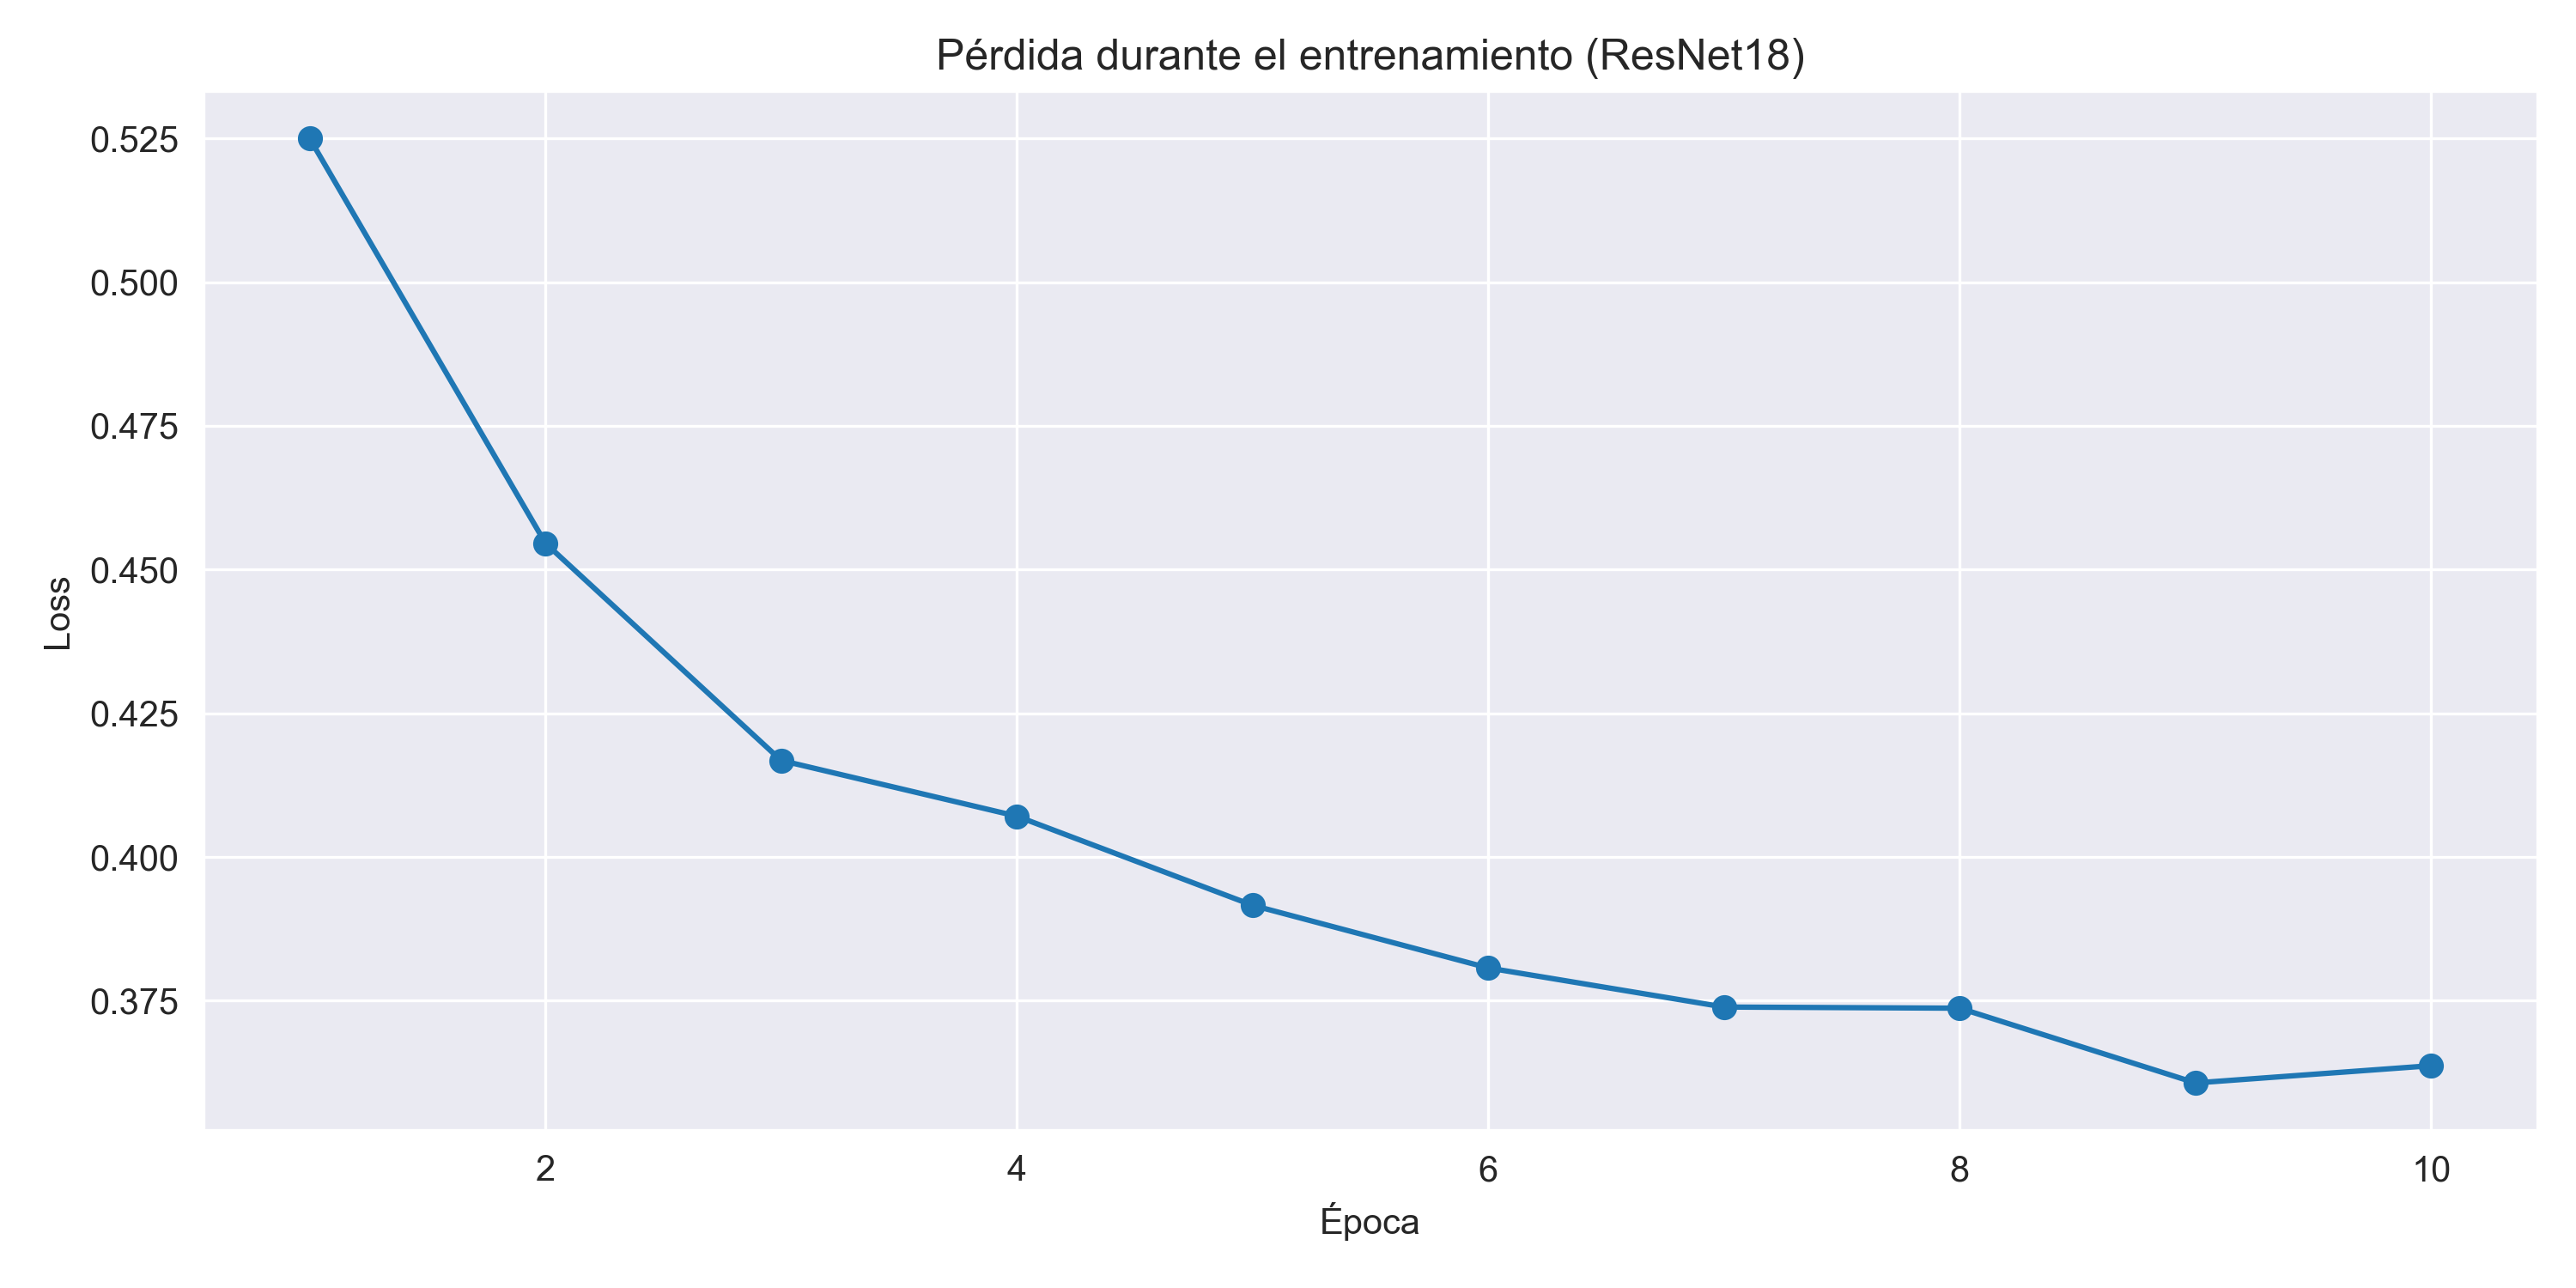
\includegraphics[width=\textwidth]{images/resnet18_loss_curve.png}
        \caption{Pèrdua durant l’entrenament.}
        \label{fig:resnet18_loss}
    \end{subfigure}
    \hfill
    \begin{subfigure}[b]{0.48\textwidth}
        \centering
        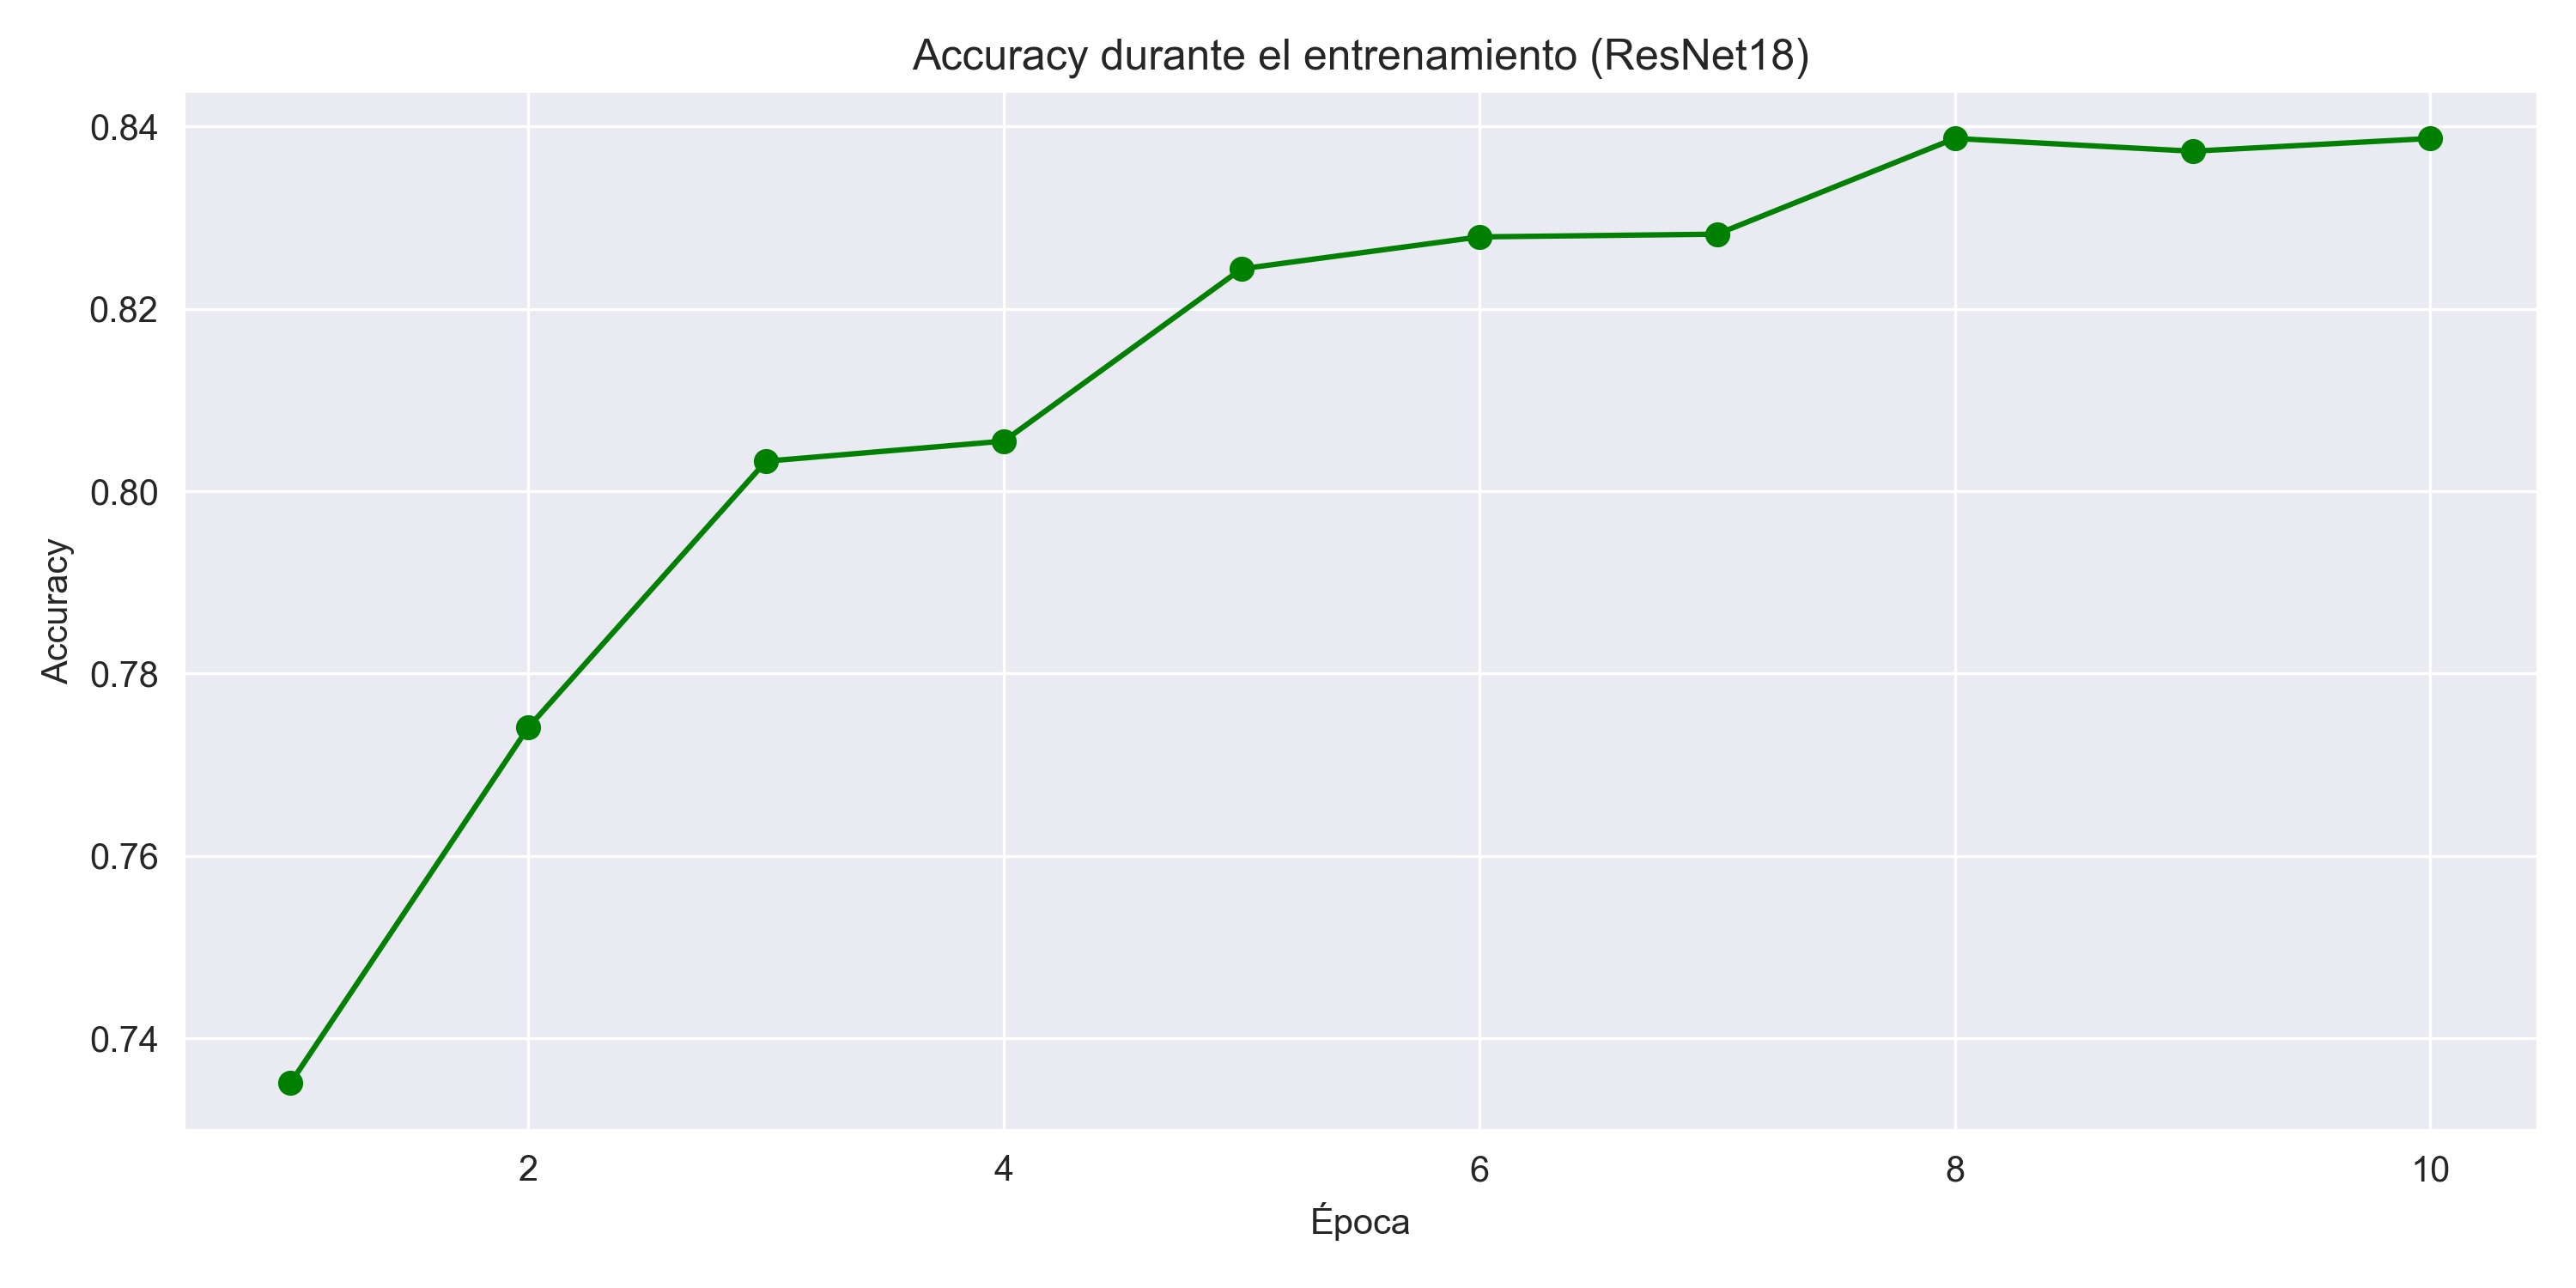
\includegraphics[width=\textwidth]{images/resnet18_accuracy_curve.png}
        \caption{Precisió durant l’entrenament.}
        \label{fig:resnet18_accuracy}
    \end{subfigure}

    \caption{Evolució de l’entrenament del model ResNet18: pèrdua (esquerra) i precisió (dreta).}
    \label{fig:resnet18_training_curves}
\end{figure}

El model convergeix ràpidament i supera des de les primeres èpoques el rendiment del
model entrenat des de zero, fet característic del transfer learning.

\subsection{Avaluació sobre el Conjunt de Test}

El \textit{classification report} obtingut va ser:

\begin{table}[h!]
\centering
\begin{tabular}{l|c|c|c|c}
\hline
\textbf{Classe} & \textbf{Precision} & \textbf{Recall} & \textbf{F1-score} & \textbf{Support} \\
\hline
0 & 0.8048 & 0.9631 & 0.8769 & 732 \\
1 & 0.8402 & 0.4537 & 0.5892 & 313 \\
\hline
\textbf{Accuracy} & \multicolumn{4}{c}{0.8105} \\
\textbf{Macro avg} & 0.8225 & 0.7084 & 0.7330 & 1045 \\
\textbf{Weighted avg} & 0.8154 & 0.8105 & 0.7907 & 1045 \\
\hline
\end{tabular}
\caption{Classification report del model ResNet18 sobre el conjunt de test.}
\label{tab:resnet_report}
\end{table}

La matriu de confusió va ser:

\begin{figure}[H]
    \centering
    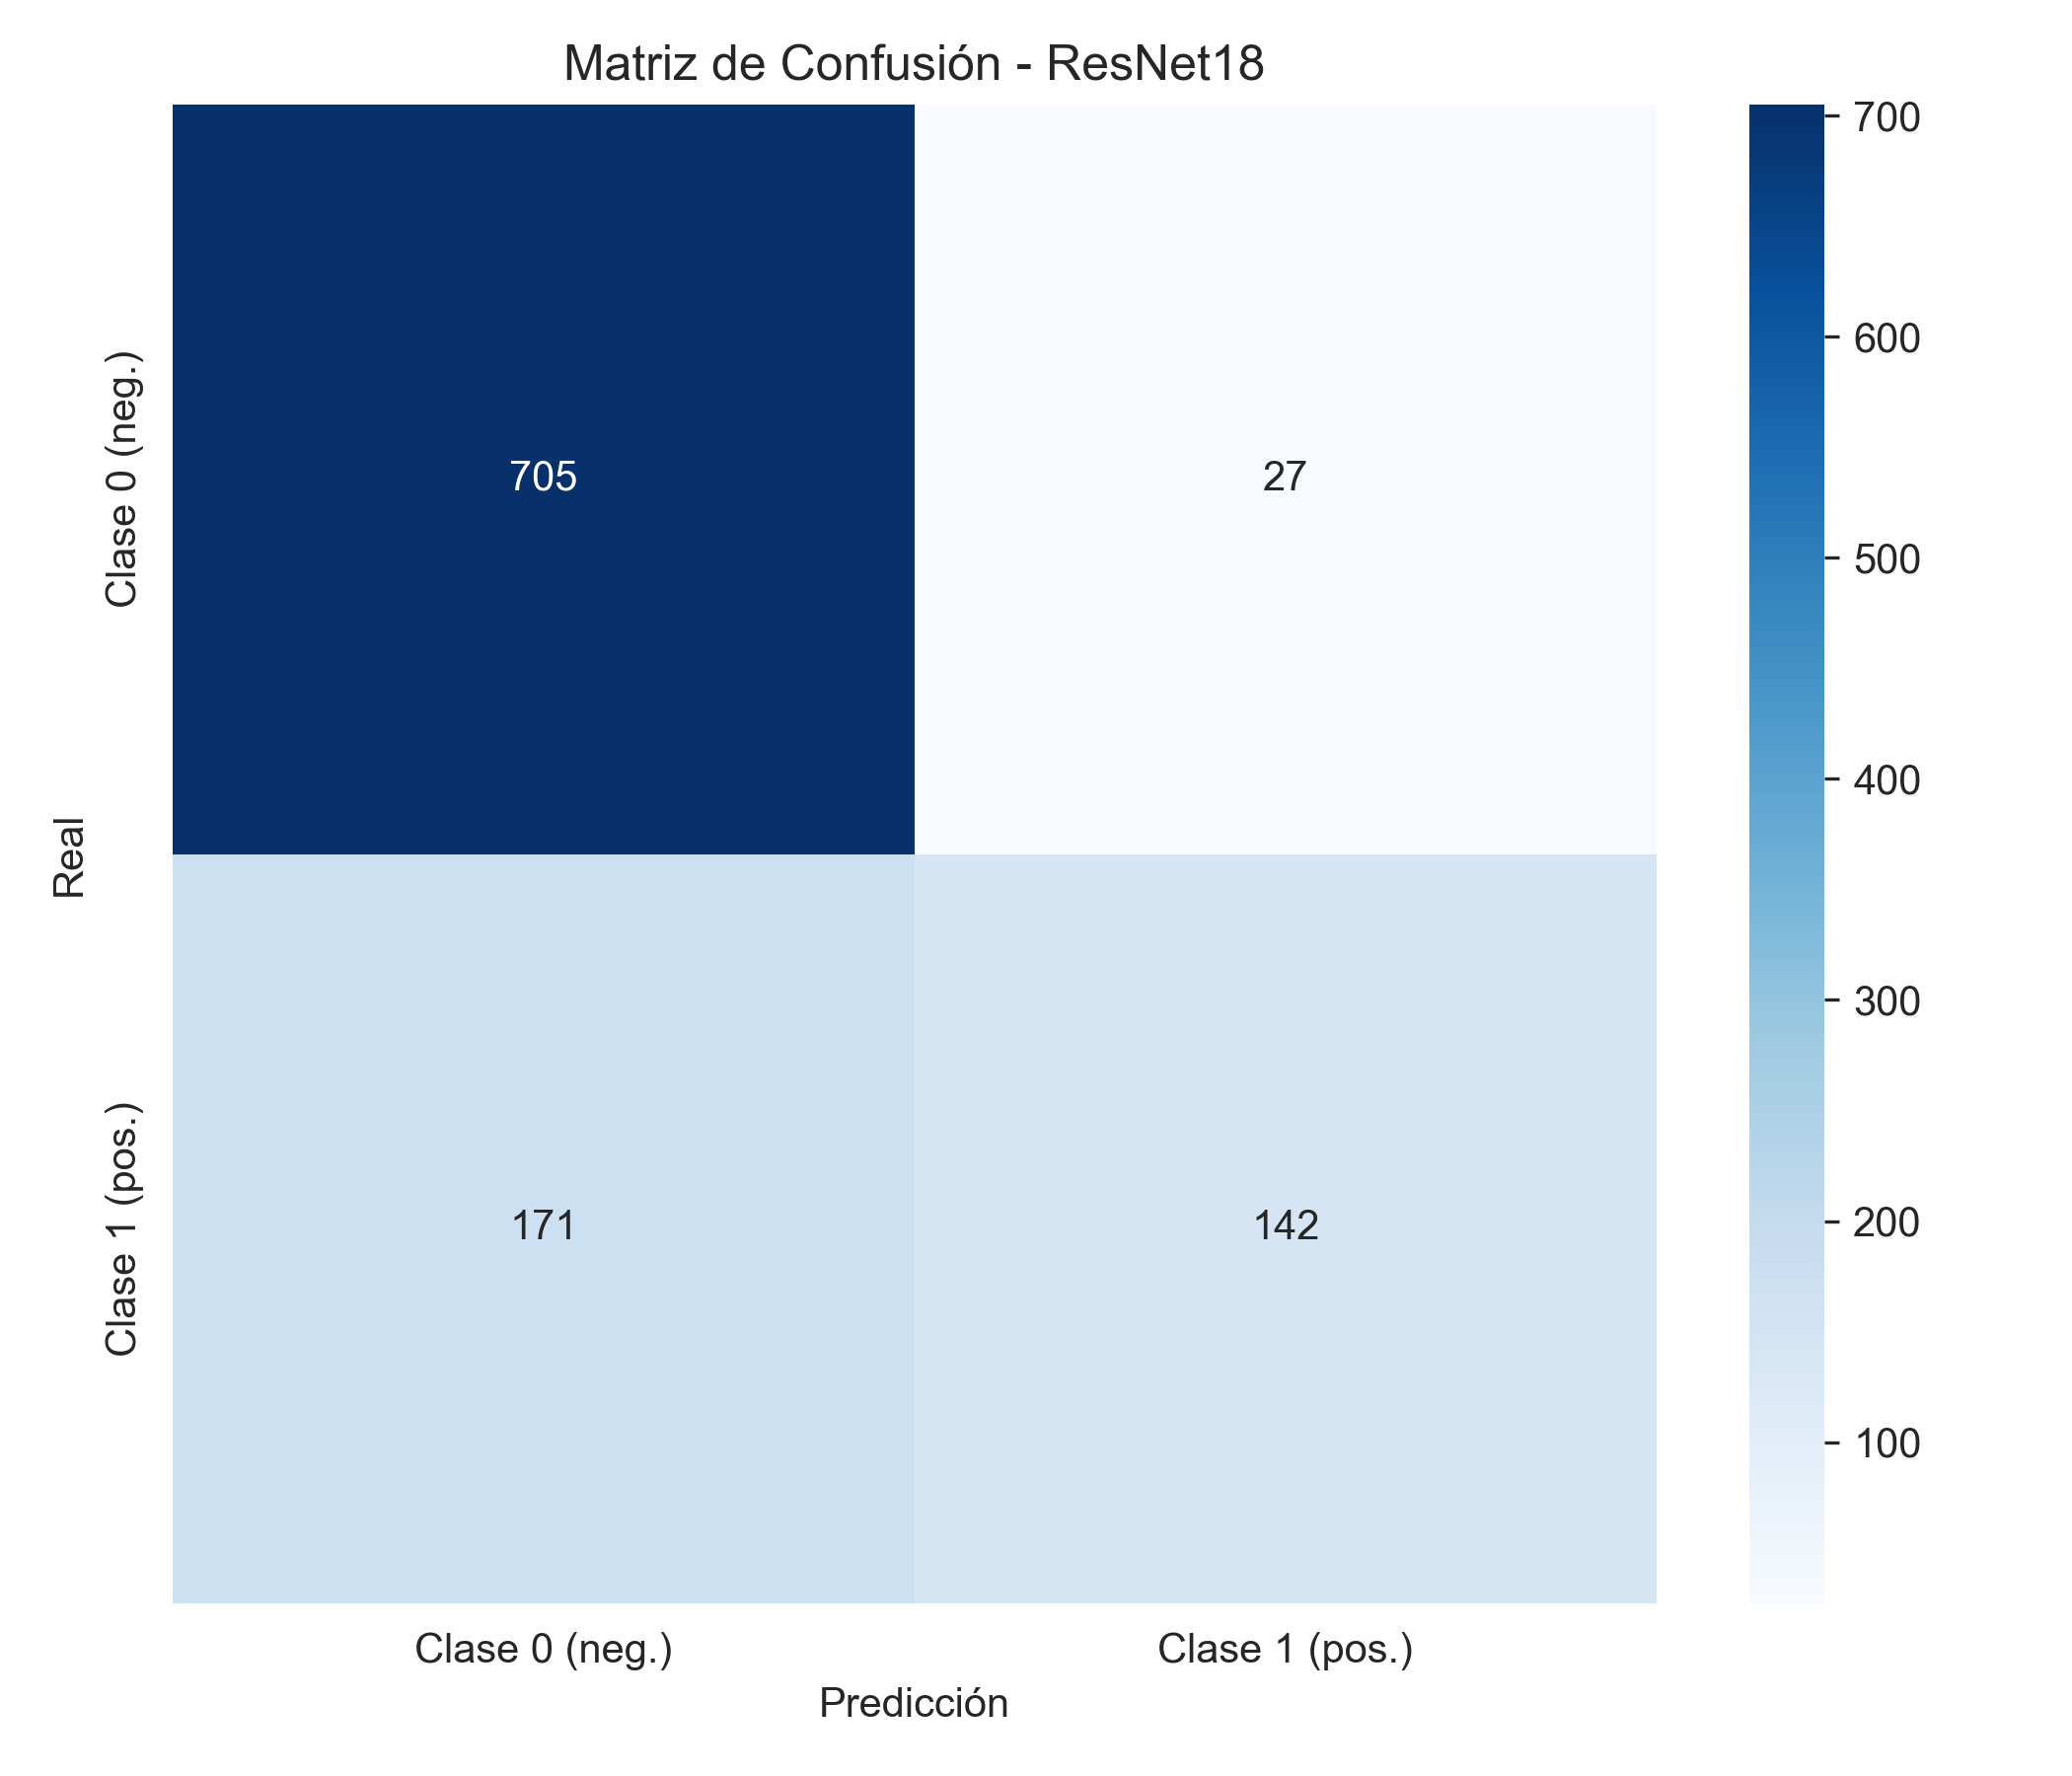
\includegraphics[width=0.70\textwidth]{images/resnet18_confusion_matrix.png}
    \caption{Matriu de confusió del model ResNet18 avaluat sobre el conjunt de test.}
    \label{fig:resnet18_confusion}
\end{figure}

\subsection{Interpretació dels Resultats}

Els resultats mostren diverses conclusions rellevants:

\begin{itemize}
    \item El model assoleix una \textbf{accuracy del 81.05\%}, superant clarament la CNN entrenada des de zero.
    \item La classe negativa (0) aconsegueix un \textbf{recall del 96.31\%}, indicant una detecció excel·lent de radiografies sense nòduls.
    \item La classe positiva (1) obté un \textbf{recall del 45.37\%}, millor que la CNN bàsica però encara insuficient per a un problema clínic on els falsos negatius són crítics.
    \item L’F1-score de la classe 1 millora respecte al model anterior, però no assoleix valors òptims a causa del desbalanceig del dataset.
\end{itemize}

Aquests resultats indiquen que l’ús de transfer learning millora la capacitat de
generalització, però l’arquitectura encara no aprofita patrons específics de les
radiografies, ja que la xarxa va ser entrenada originalment amb imatges naturals.


\section{Model 3: Transfer Learning amb DenseNet121}

Després d’avaluar ResNet18, es va utilitzar una arquitectura més avançada i amb
connexions més denses: \textbf{DenseNet121}. Aquest model és àmpliament emprat en
radiologia digital a causa de la seva capacitat per reutilitzar característiques entre
capes, fet que millora l’eficiència del gradient i la propagació de la informació.
L’objectiu d’aquest experiment és analitzar com un model més profund i amb una major
capacitat representacional afecta el rendiment en la detecció de nòduls pulmonars.

\subsection{Preparació del Dataset}

La preparació del dataset va ser idèntica a la utilitzada amb ResNet18. Totes les imatges
en format MHA es van normalitzar en el rang $[0,1]$, es van redimensionar a $224\times224$
i es va replicar el canal únic en tres canals RGB per adaptar-se al format requerit per
DenseNet121 preentrenada a ImageNet.

El Dataset emprat és:

\begin{lstlisting}[style=mypython]
img = img_np.astype(np.float32)
img = (img - img.min()) / (img.max() - img.min())
img = cv2.resize(img, (224,224))
img = np.expand_dims(img, axis=0)
img = np.repeat(img, 3, axis=0)  # (3,H,W)
\end{lstlisting}

Després de filtrar imatges inexistents, el conjunt final va quedar en:

\[
\text{Total: }5224, \quad
\text{Train: }4179, \quad
\text{Test: }1045.
\]

\subsection{Arquitectura i Transfer Learning}

DenseNet121 es va carregar amb pesos preentrenats a ImageNet. Totes les capes es van
congelar per preservar l’extractor de característiques, modificant únicament el
classificador final:

\begin{lstlisting}[style=mypython]
model = models.densenet121(
    weights=models.DenseNet121_Weights.IMAGENET1K_V1
)

for param in model.parameters():
    param.requires_grad = False

num_features = model.classifier.in_features
model.classifier = nn.Linear(num_features, 2)
\end{lstlisting}

D’aquesta manera, únicament es van entrenar els pesos necessaris per adaptar el model a
la classificació binària de NODE21.

\subsection{Entrenament}

L’entrenament es va realitzar durant 10 èpoques utilitzant:

\begin{itemize}
    \item Optimitzador Adam ($lr = 1 \times 10^{-3}$)
    \item Funció de pèrdua: CrossEntropy
    \item Batch size: 32
    \item Execució en GPU
\end{itemize}

Els resultats per època van ser:

\begin{table}[h!]
\centering
\begin{tabular}{c|c|c}
\hline
\textbf{Època} & \textbf{Loss} & \textbf{Accuracy} \\
\hline
1 & 0.5052 & 0.7550 \\
2 & 0.4152 & 0.8057 \\
3 & 0.3866 & 0.8284 \\
4 & 0.3594 & 0.8480 \\
5 & 0.3593 & 0.8385 \\
6 & 0.3353 & 0.8571 \\
7 & 0.3398 & 0.8500 \\
8 & 0.3359 & 0.8509 \\
9 & 0.3154 & 0.8641 \\
10 & 0.3036 & 0.8729 \\
\hline
\end{tabular}
\caption{Pèrdua i exactitud per època del model DenseNet121.}
\label{tab:densenet121_training}
\end{table}

\begin{figure}[H]
    \centering
    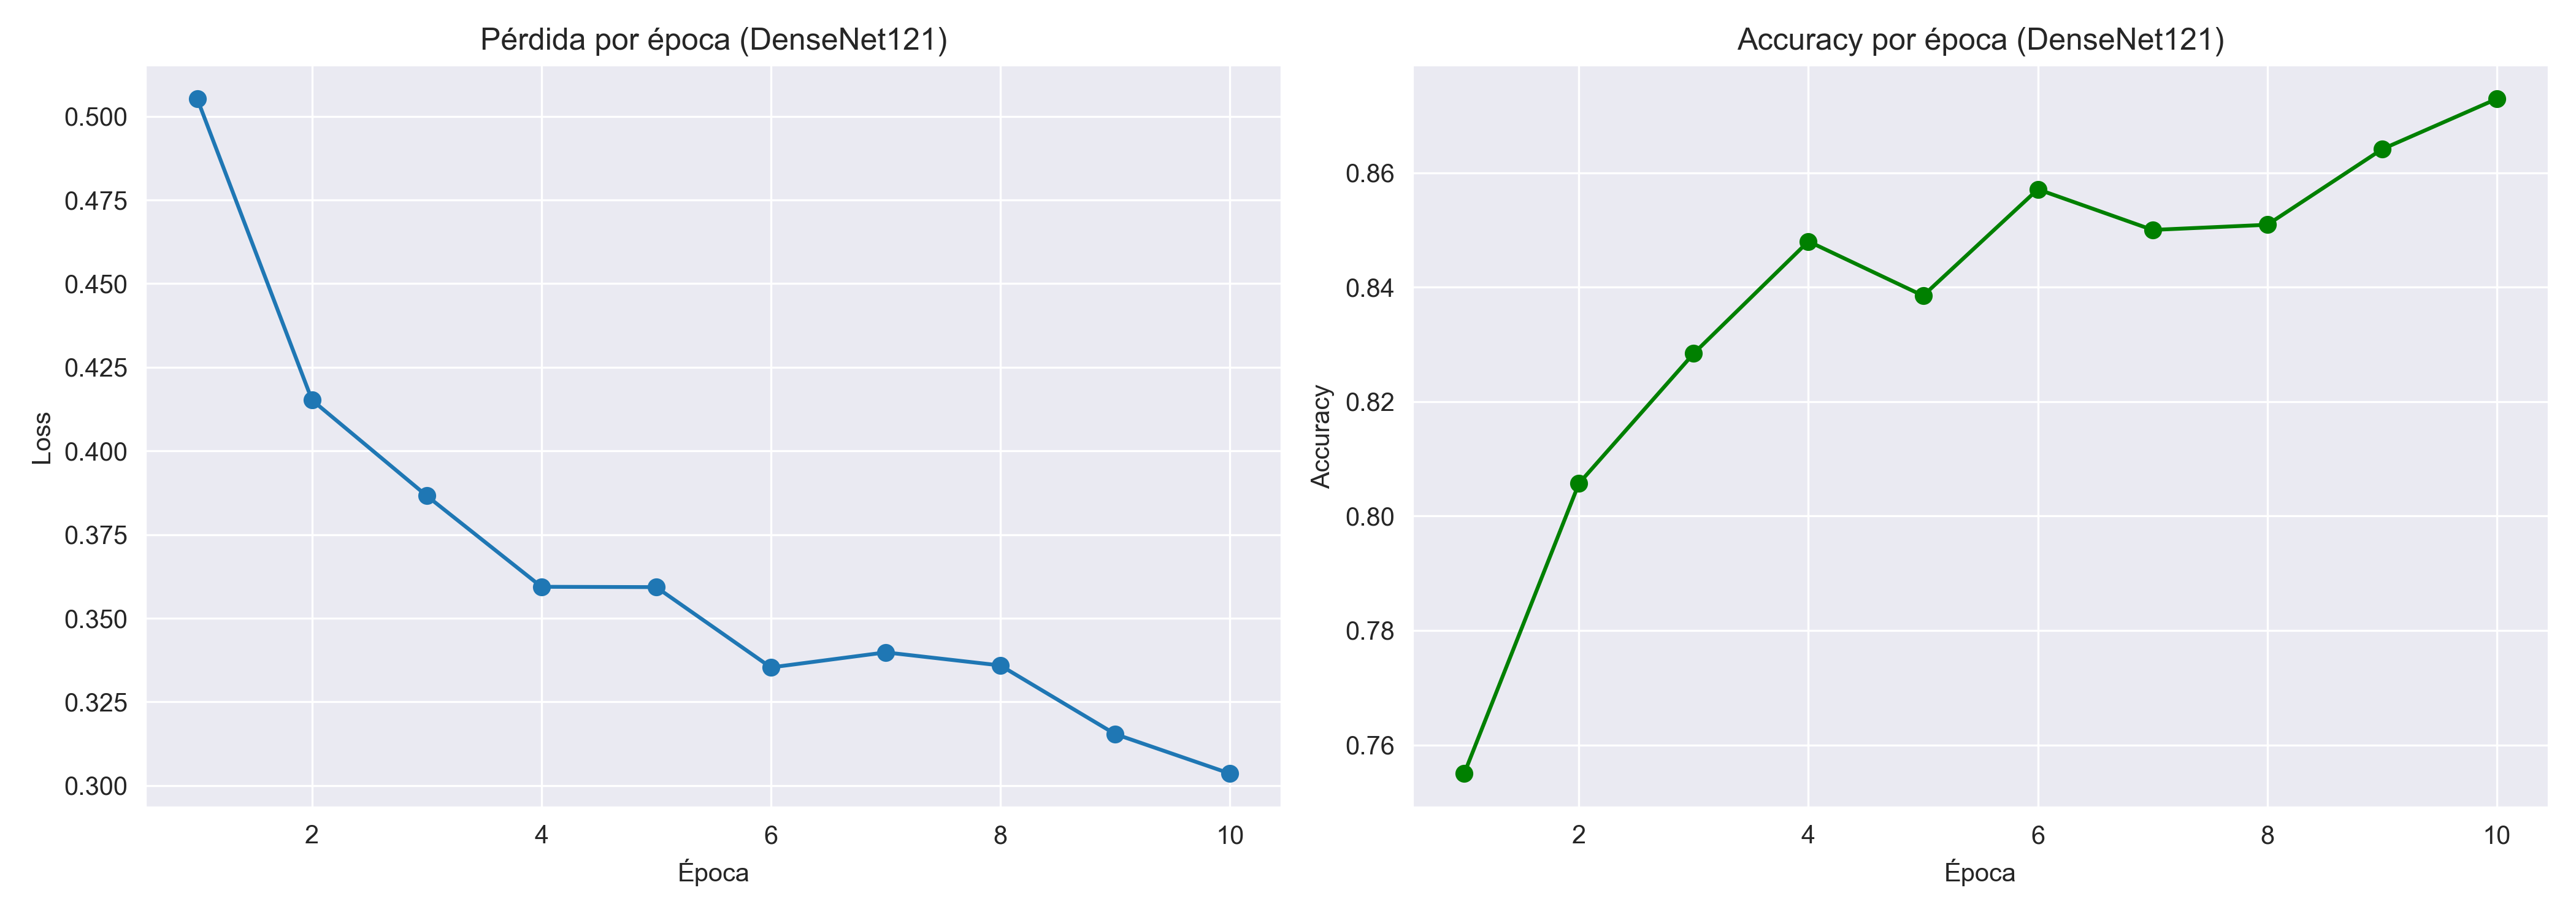
\includegraphics[width=0.90\textwidth]{images/densenet121_training_curves.png}
    \caption{Evolució conjunta de la pèrdua (\textit{loss}) i de la precisió (\textit{accuracy}) del model DenseNet121 durant l’entrenament.}
    \label{fig:densenet121_training_curves}
\end{figure}

El model mostra una clara tendència a la millora contínua, estabilitzant-se en valors de
precisió superiors al 87\% durant l’entrenament.

\subsection{Avaluació sobre el Conjunt de Test}

El rendiment final sobre el conjunt de test va ser:

\[
\text{Accuracy}_{test} = 0.8459.
\]

El \textit{classification report} complet va ser:

\begin{table}[H]
\centering
\begin{tabular}{l|c|c|c|c}
\hline
\textbf{Classe} & \textbf{Precision} & \textbf{Recall} & \textbf{F1-score} & \textbf{Support} \\
\hline
0 & 0.8781 & 0.9057 & 0.8917 & 732 \\
1 & 0.7621 & 0.7061 & 0.7330 & 313 \\
\hline
\textbf{Accuracy} & \multicolumn{4}{c}{0.8459} \\
\textbf{Macro avg} & 0.8201 & 0.8059 & 0.8124 & 1045 \\
\textbf{Weighted avg} & 0.8434 & 0.8459 & 0.8442 & 1045 \\
\hline
\end{tabular}
\caption{Classification report del model DenseNet121.}
\label{tab:densenet121_report}
\end{table}

La matriu de confusió obtinguda va ser:

\begin{figure}[H]
    \centering
    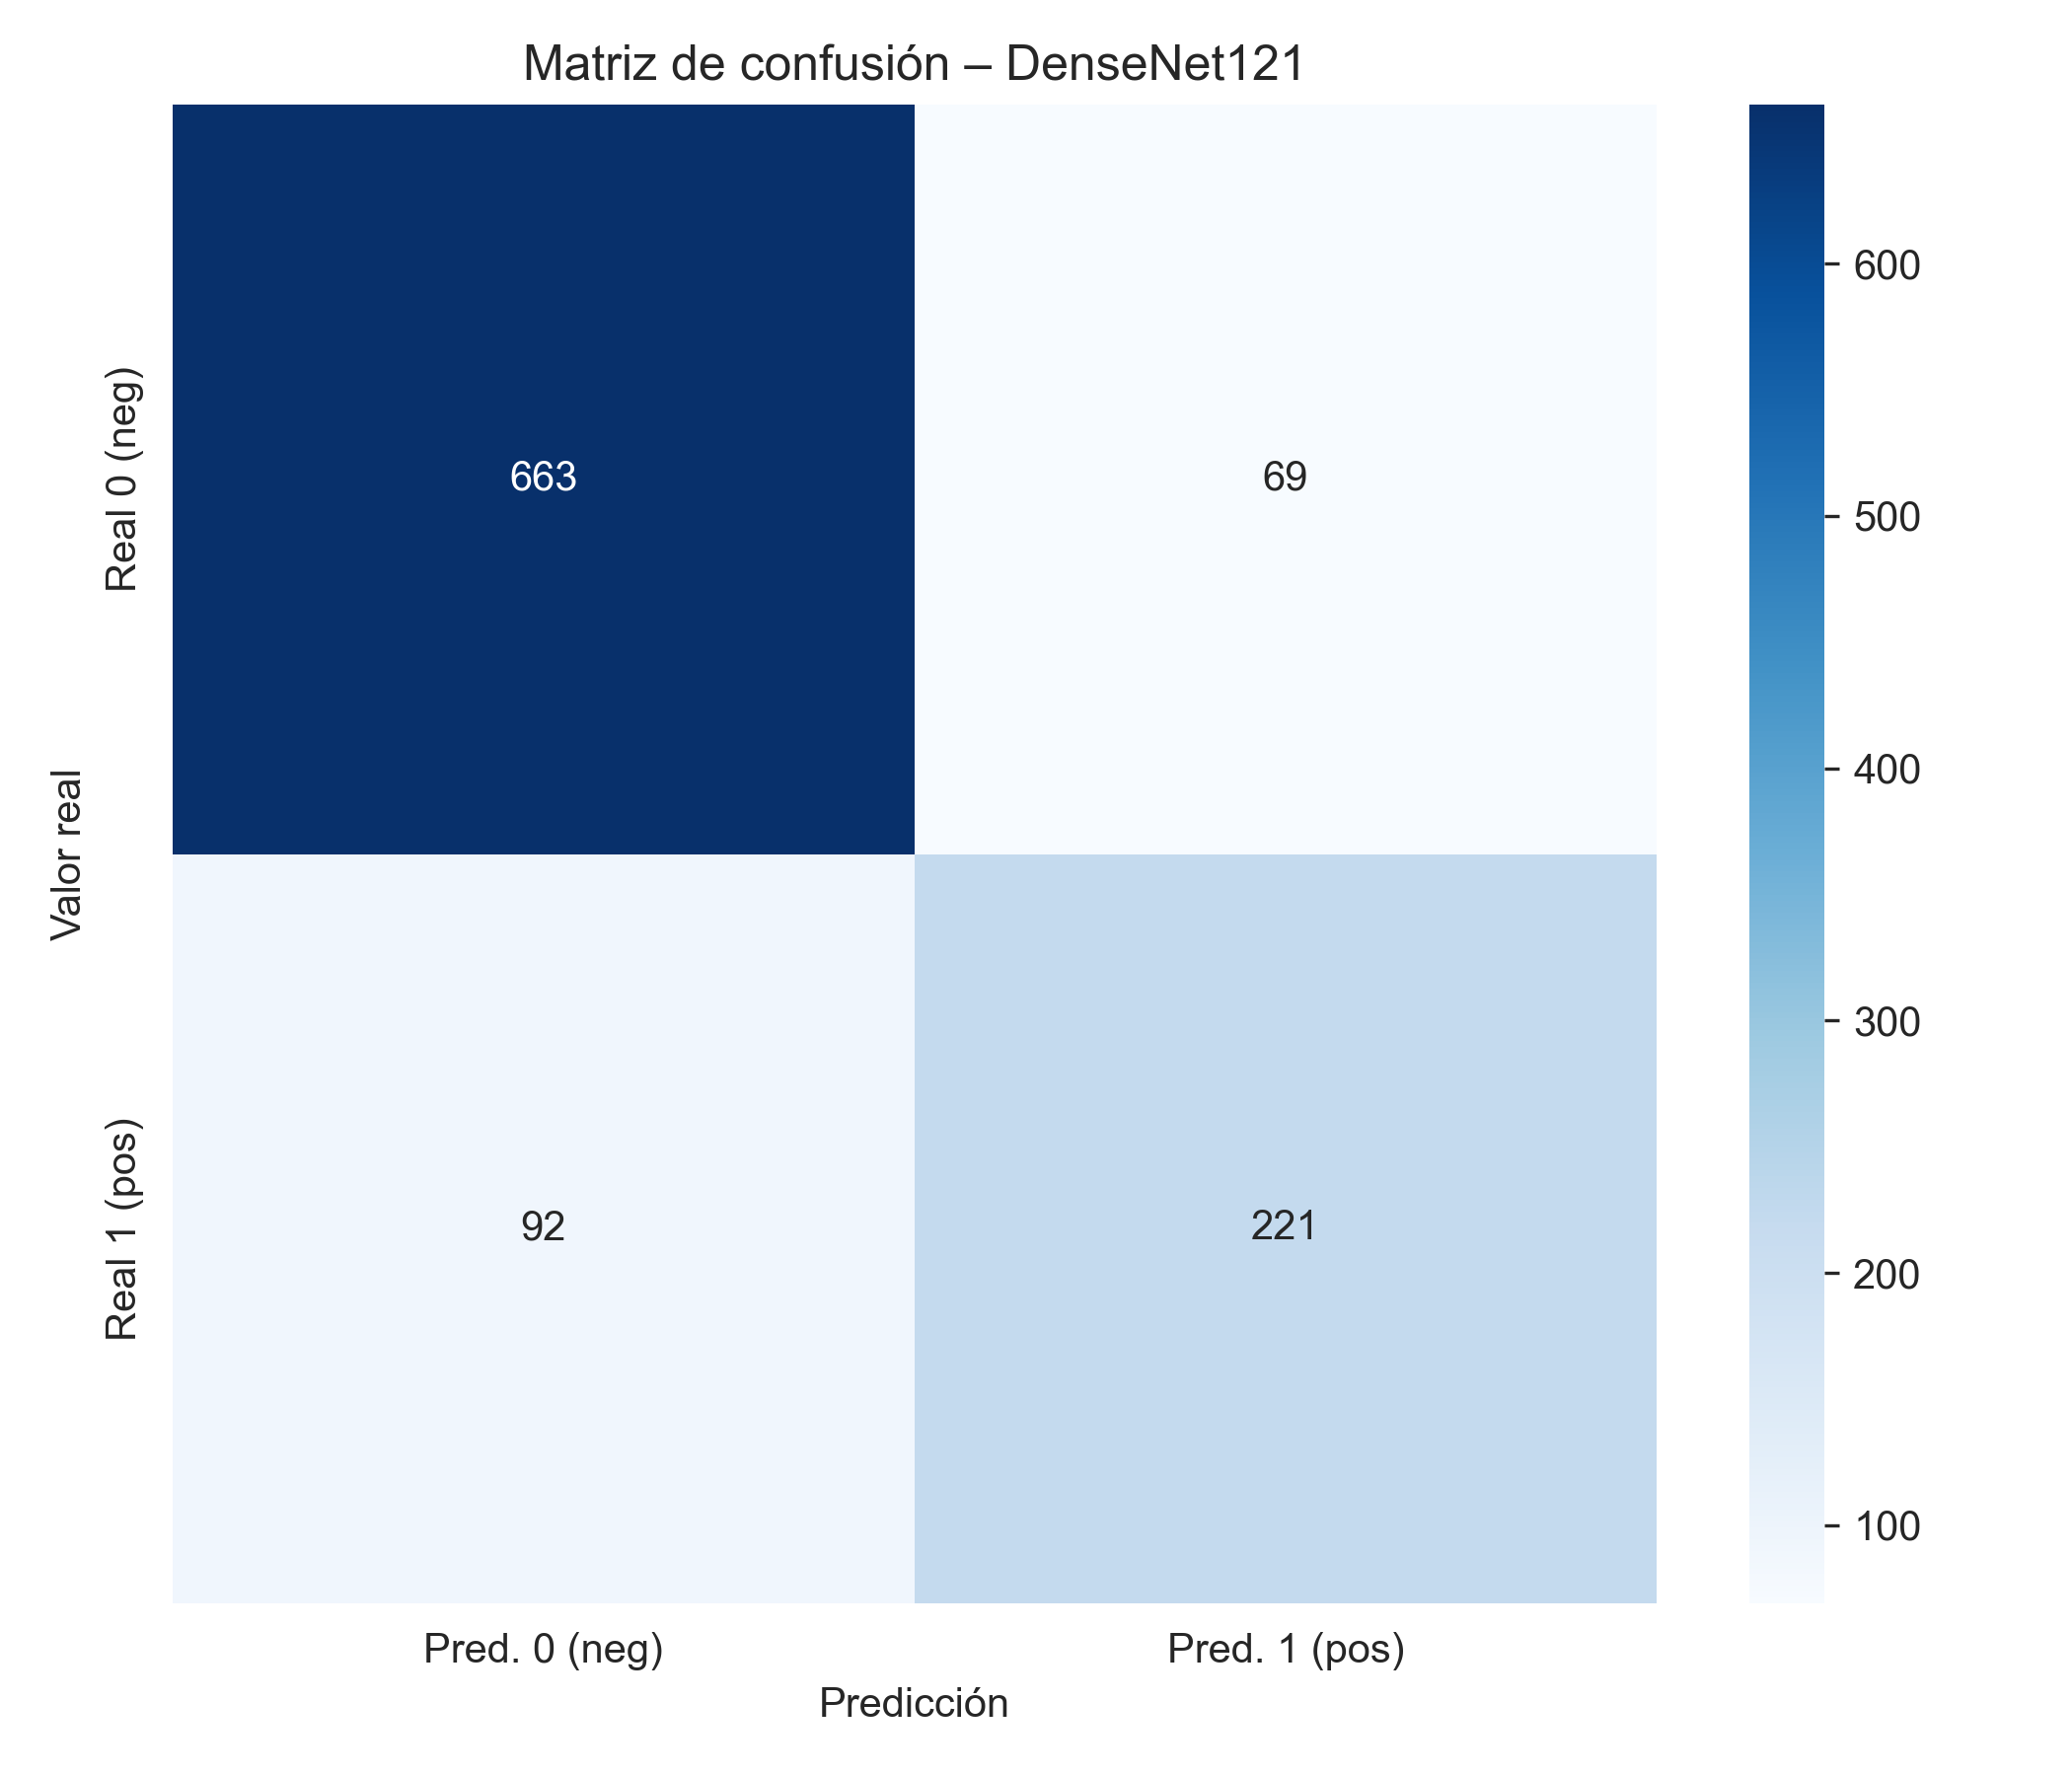
\includegraphics[width=0.65\textwidth]{images/densenet121_confusion_matrix.png}
    \caption{Matriu de confusió del model DenseNet121 avaluat sobre el conjunt de test.}
    \label{fig:densenet121_confusion}
\end{figure}
la qual cosa indica que la classe positiva (1) millora respecte a ResNet18, especialment
en \textit{recall} i \textit{F1-score}.

\subsection{Anàlisi del Rendiment}

DenseNet121 ofereix els millors resultats fins al moment:

\begin{itemize}
    \item La classe negativa (0) presenta un \textit{recall} del 90.57\%, amb molt pocs falsos positius.
    \item La classe positiva (1) millora el seu F1-score fins a 0.7330, superant clarament ResNet18 (0.5892).
    \item L’\textit{accuracy} global puja fins al 84.59\%, la més alta entre els models avaluats.
\end{itemize}

Aquest comportament és coherent amb l’arquitectura DenseNet, que aprofita connexions
denses entre capes per evitar la pèrdua de gradient i millorar la reutilització de
característiques.

\subsection{Figures recomanades}

Es recomana incloure les següents gràfiques (generades prèviament en Python):

\begin{itemize}
    \item Corba de pèrdua per època.
    \item Corba de precisió per època.
    \item Matriu de confusió en format imatge.
\end{itemize}

Aquestes visualitzacions permeten avaluar de manera intuïtiva l’estabilitat de
l’entrenament i els patrons d’error del model.



\section{Model 4: Transfer Learning amb EfficientNet-B0}

Després d’avaluar ResNet18 i DenseNet121, es va entrenar un quart model basat en
l’arquitectura \textbf{EfficientNet-B0}, coneguda per la seva elevada relació
rendiment–eficiència gràcies al seu escalat compost de profunditat, amplada i
resolució. Aquest model és especialment adequat per a imatges mèdiques amb estructura
subtil, com les radiografies de tòrax.

\subsection{Preparació del Dataset}

La preparació de les imatges segueix el mateix procediment utilitzat en els models
anteriors: normalització en el rang $[0,1]$, redimensionat a $224\times224$ i
replicació del canal únic en tres canals RGB per adaptar-se als pesos
preentrenats a ImageNet.

\begin{lstlisting}[style=mypython]
img = img_np.astype(np.float32)
img = (img - img.min()) / (img.max() - img.min())
img = cv2.resize(img, (224,224))
img = np.expand_dims(img, axis=0)
img = np.repeat(img, 3, axis=0)  # (3,H,W)
\end{lstlisting}

El dataset final consta de:

\[
\text{Train: }4179, \qquad
\text{Test: }1045, \qquad
\text{Total vàlides: }5224.
\]

\subsection{Arquitectura i Transfer Learning}

EfficientNet-B0 es va carregar amb pesos preentrenats a ImageNet. Es van congelar totes
les capes de l’extractor de característiques, substituint únicament la capa final del
classificador per ajustar-lo a dues classes:

\begin{lstlisting}[style=mypython]
model = models.efficientnet_b0(
    weights=models.EfficientNet_B0_Weights.IMAGENET1K_V1
)

for param in model.parameters():
    param.requires_grad = False

num_features = model.classifier[1].in_features
model.classifier[1] = nn.Linear(num_features, 2)
\end{lstlisting}

Això permet entrenar únicament l’última capa, reduint el risc de sobreajust
en datasets petits com NODE21.

\subsection{Entrenament}

El model es va entrenar durant 10 èpoques amb:

\begin{itemize}
    \item Optimitzador Adam ($lr = 1 \times 10^{-3}$)
    \item Funció de pèrdua CrossEntropy
    \item Batch size 32
    \item Execució en GPU
\end{itemize}

Els resultats per època van ser:

\begin{table}[h!]
\centering
\begin{tabular}{c|c|c}
\hline
\textbf{Època} & \textbf{Loss} & \textbf{Accuracy} \\
\hline
1 & 0.4593 & 0.7875 \\
2 & 0.3842 & 0.8303 \\
3 & 0.3467 & 0.8531 \\
4 & 0.3466 & 0.8543 \\
5 & 0.3364 & 0.8626 \\
6 & 0.3226 & 0.8653 \\
7 & 0.3246 & 0.8650 \\
8 & 0.3233 & 0.8588 \\
9 & 0.3146 & 0.8660 \\
10 & 0.3191 & 0.8626 \\
\hline
\end{tabular}
\caption{Pèrdua i exactitud per època del model EfficientNet-B0.}
\label{tab:efficientnet_training}
\end{table}

\begin{figure}[H]
    \centering
    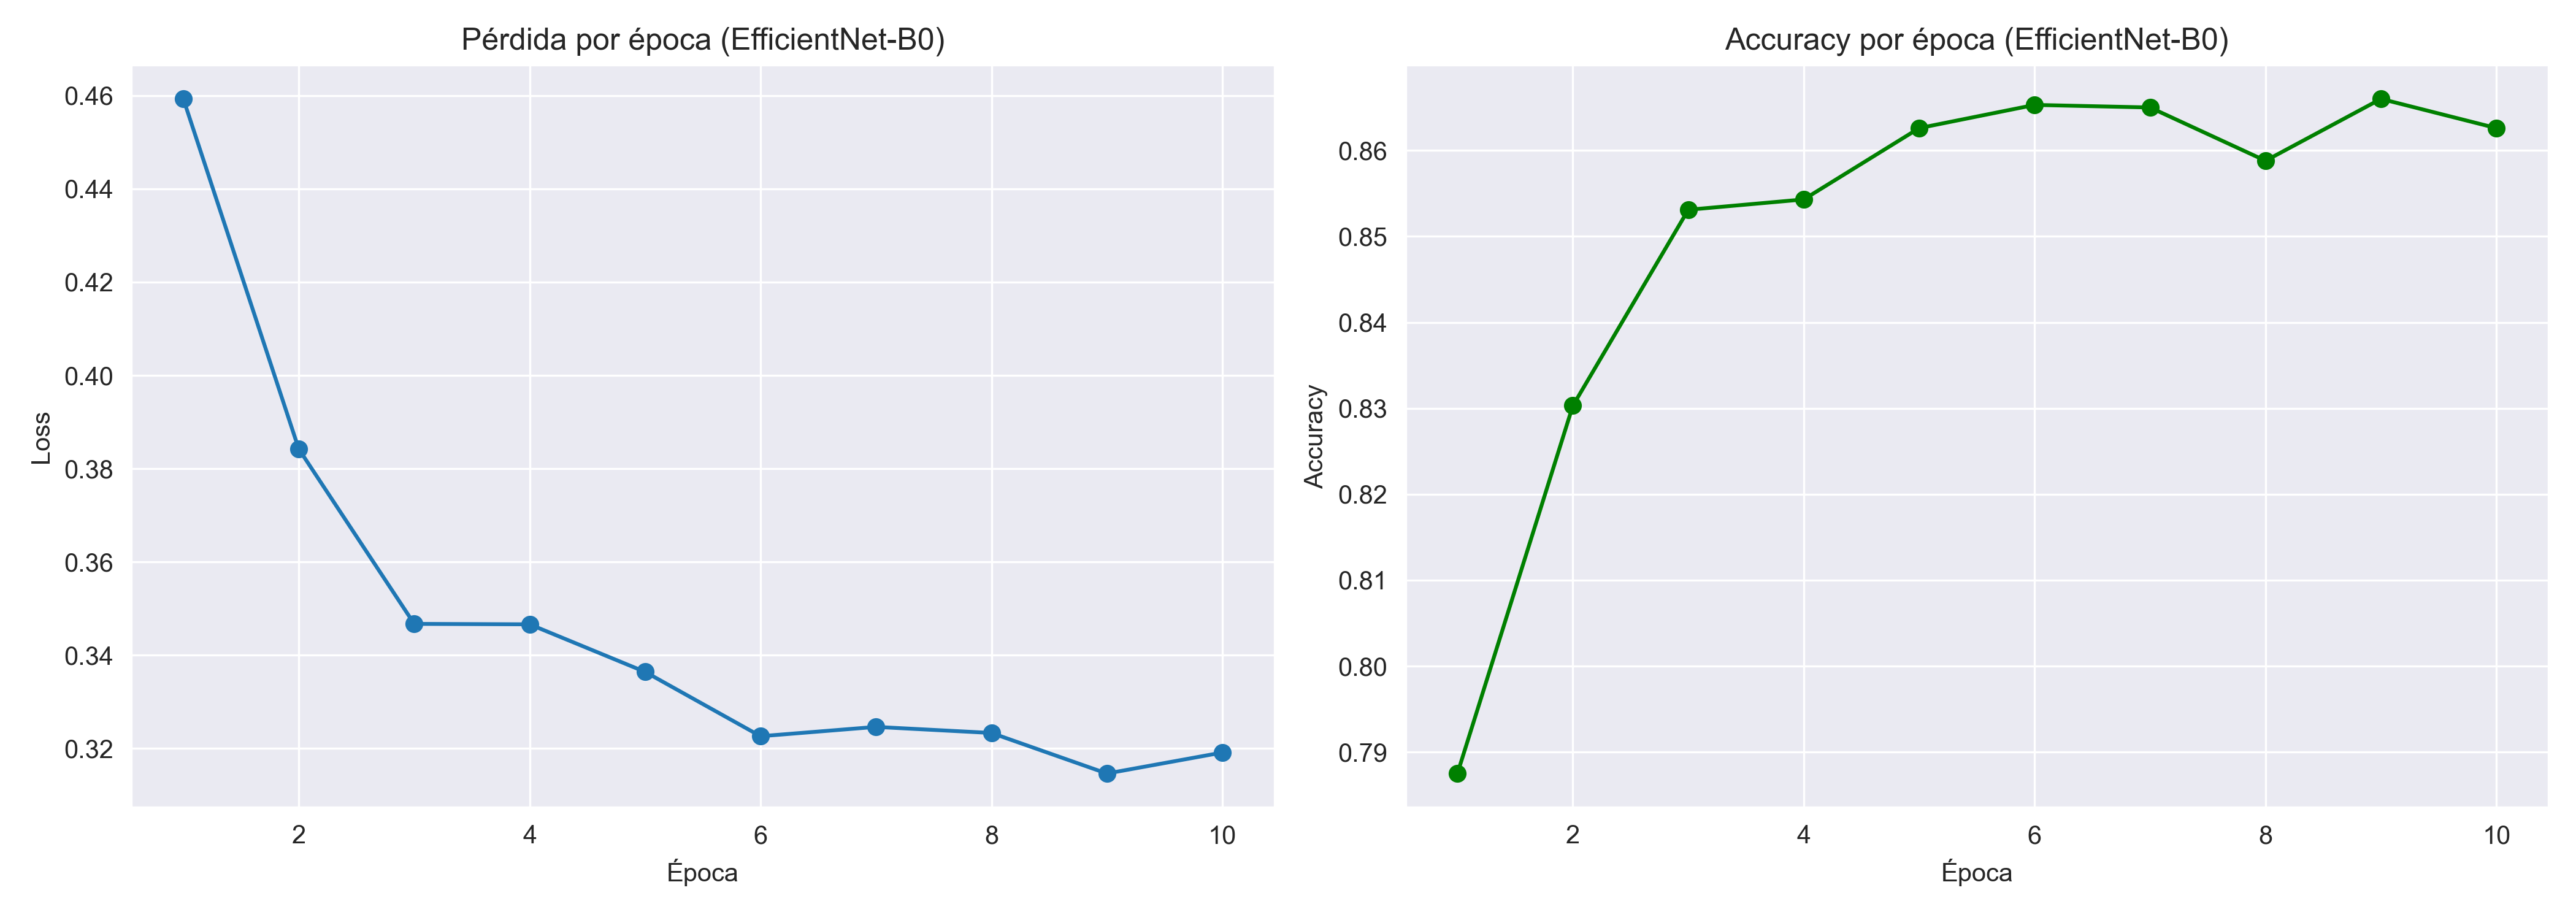
\includegraphics[width=0.90\textwidth]{images/efficientnet_training_curves.png}
    \caption{Evolució de la pèrdua (\textit{loss}) i de la precisió (\textit{accuracy}) durant l’entrenament del model EfficientNet-B0.}
    \label{fig:efficientnet_training_curves}
\end{figure}

El model convergeix de forma estable i millora consistentment a DenseNet121.

\subsection{Avaluació sobre el Conjunt de Test}

El rendiment final obtingut va ser:

\[
\text{Accuracy}_{test} = 0.8603
\]

superant així tots els models previs.

El \textit{classification report} va ser el següent:

\begin{table}[h!]
\centering
\begin{tabular}{l|c|c|c|c}
\hline
\textbf{Classe} & \textbf{Precision} & \textbf{Recall} & \textbf{F1-score} & \textbf{Support} \\
\hline
0 & 0.8747 & 0.9344 & 0.9036 & 732 \\
1 & 0.8175 & 0.6869 & 0.7465 & 313 \\
\hline
\textbf{Accuracy} & \multicolumn{4}{c}{0.8603} \\
\textbf{Macro avg} & 0.8461 & 0.8107 & 0.8250 & 1045 \\
\textbf{Weighted avg} & 0.8576 & 0.8603 & 0.8565 & 1045 \\
\hline
\end{tabular}
\caption{Classification report del model EfficientNet-B0.}
\label{tab:efficientnet_report}
\end{table}

La matriu de confusió va ser:

\begin{figure}[H]
    \centering
    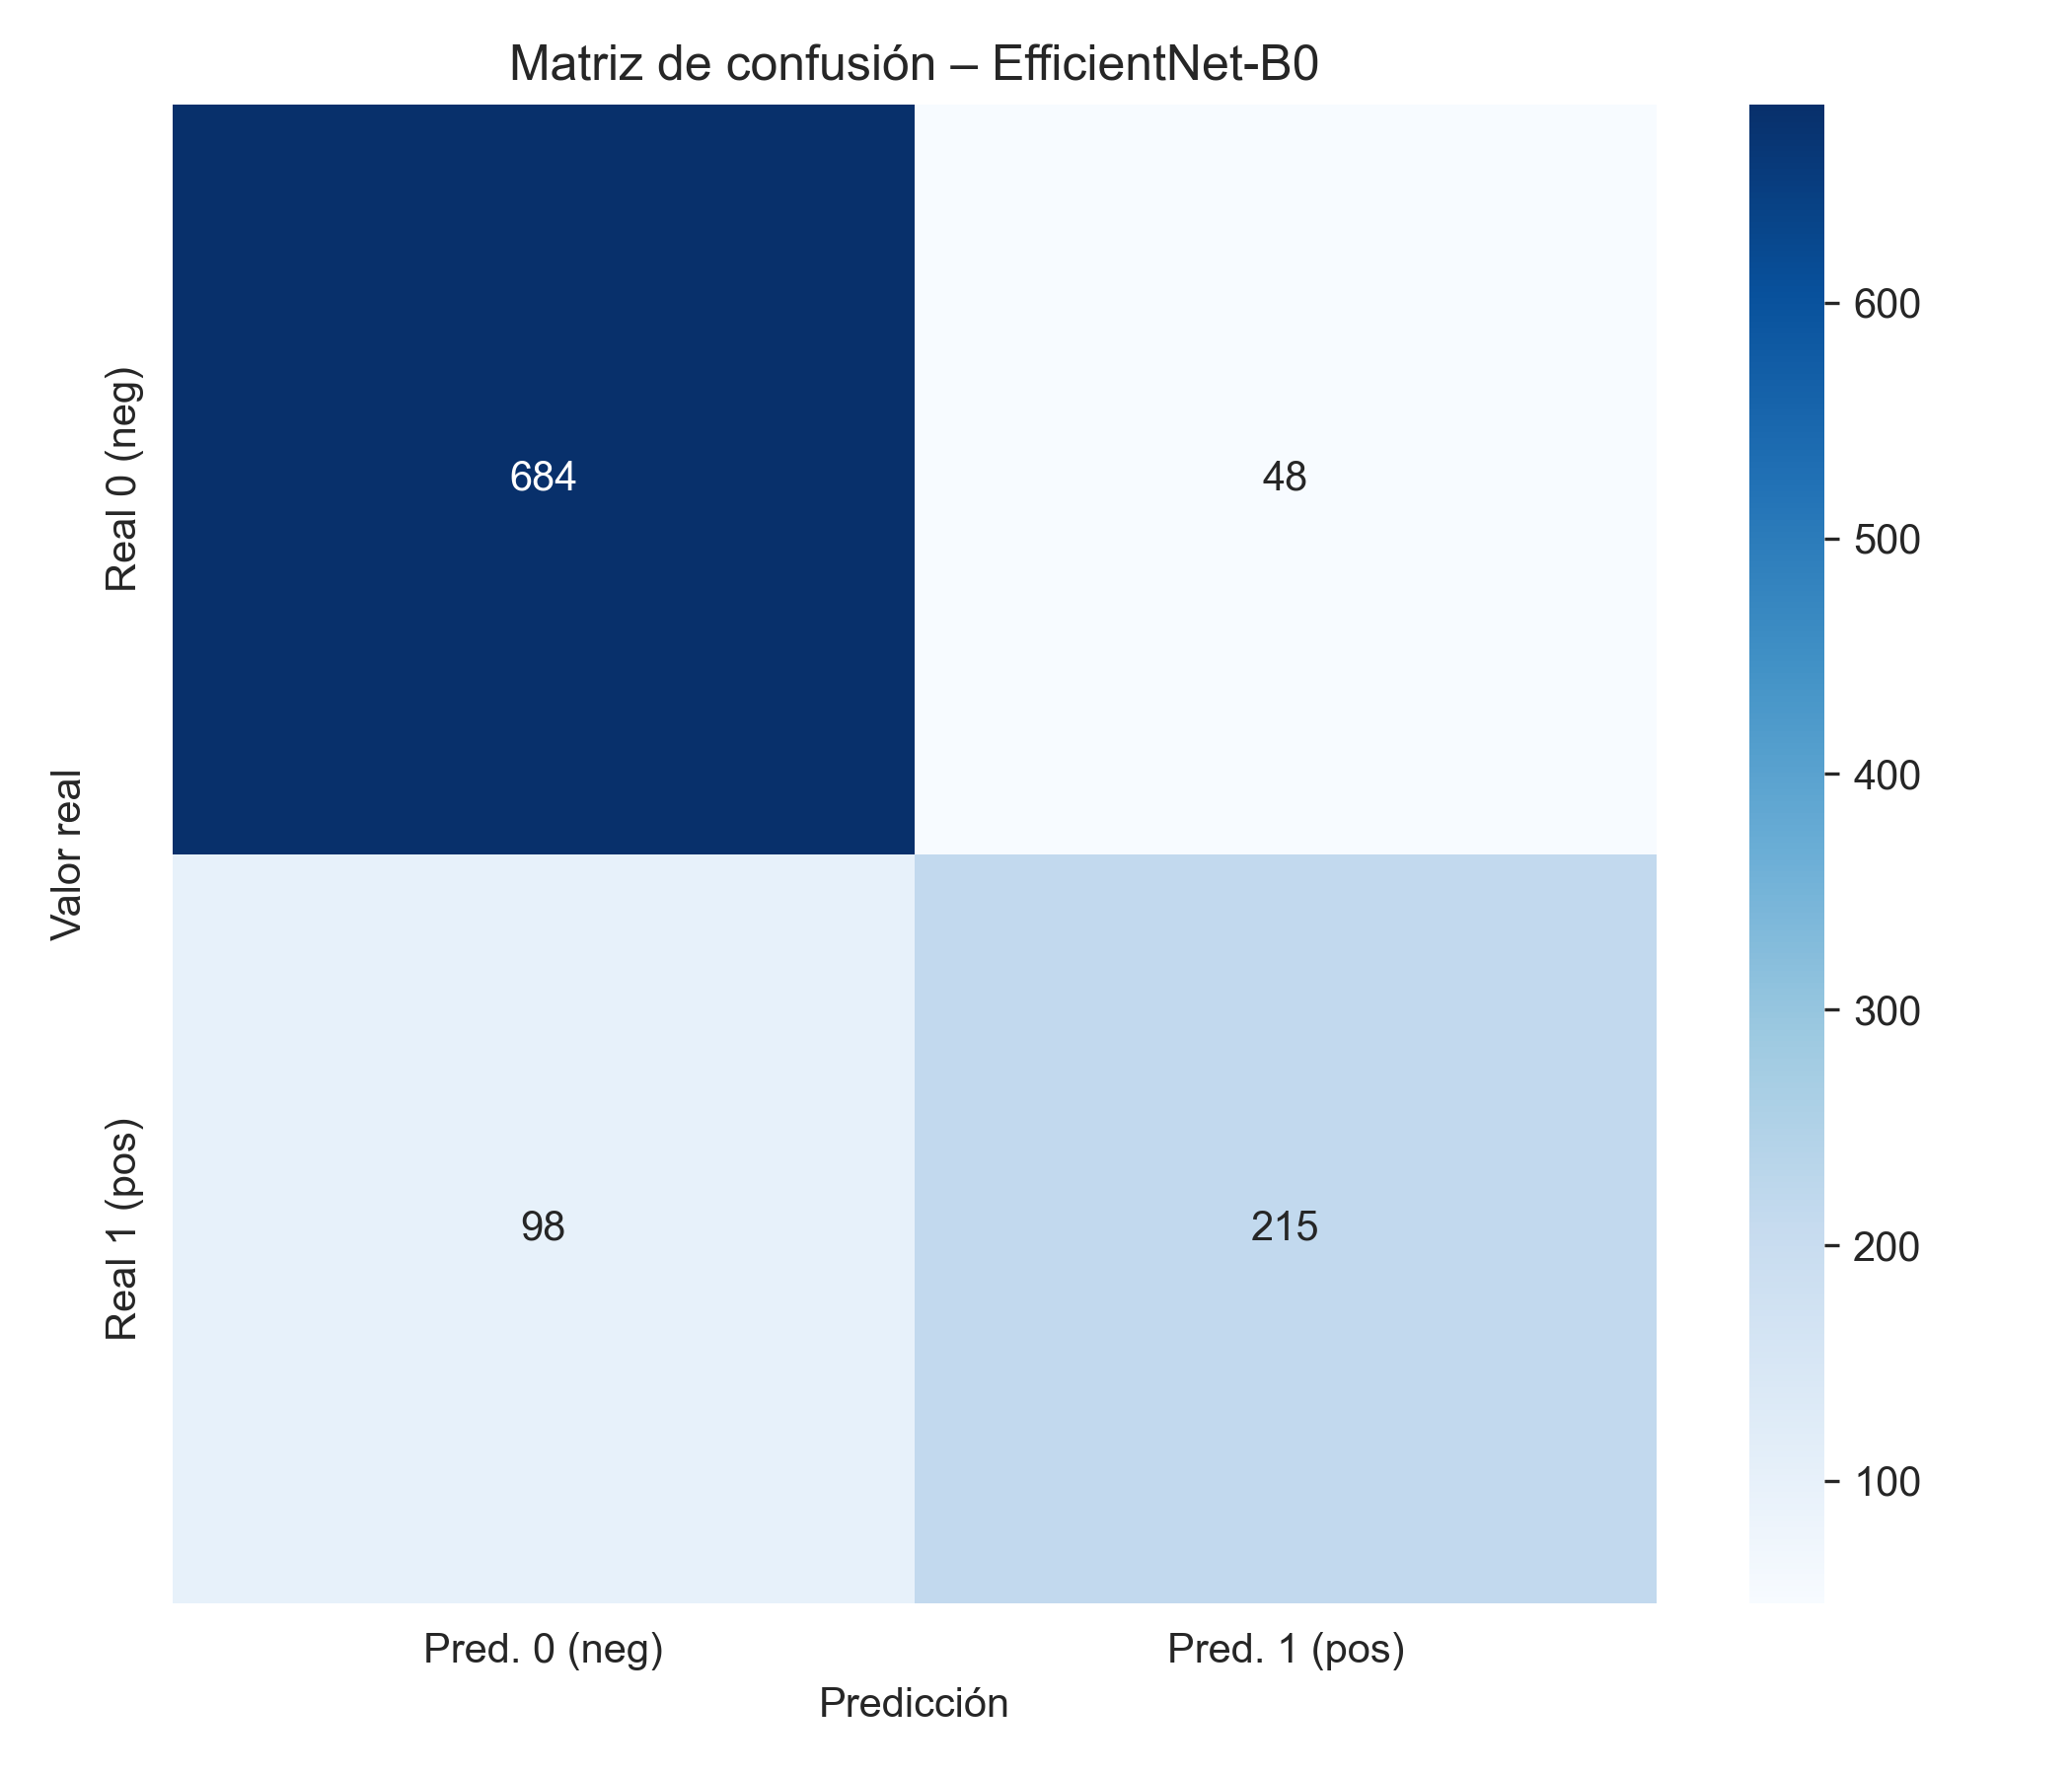
\includegraphics[width=0.65\textwidth]{images/efficientnet_confusion_matrix.png}
    \caption{Matriu de confusió del model EfficientNet-B0 avaluat sobre el conjunt de test.}
    \label{fig:efficientnet_confusion}
\end{figure}

\subsection{Anàlisi del Rendiment}

EfficientNet-B0 aconsegueix el millor rendiment entre els models basats en transfer learning:

\begin{itemize}
    \item Alt \textit{recall} de la classe negativa (93.44\%), indicant molt pocs falsos positius.
    \item Bon rendiment en la classe positiva, amb un \textit{recall} del 68.69\% i un F1-score de 0.7465.
    \item \textit{Accuracy} global del 86.03\%, la millor fins a aquesta etapa.
\end{itemize}

Aquests resultats confirmen que EfficientNet és més eficaç que ResNet18 i DenseNet121
quan l’objectiu és detectar estructures petites i subtils com els nòduls
pulmonars, fins i tot quan s’empra directament el canal d’intensitat sense
processament multicanal.

\section{Model 5: Transfer Learning amb EfficientNet-B3}

Després dels bons resultats obtinguts amb EfficientNet-B0, es va avaluar un model més
capaç dins de la mateixa família: \textbf{EfficientNet-B3}. Aquesta variant presenta una
major profunditat, amplada i resolució interna, la qual cosa permet representar patrons
més complexos en imatges mèdiques. L’objectiu d’aquest experiment era analitzar si un
model amb major capacitat podia millorar el rendiment assolit amb EfficientNet-B0
mantenint el mateix pipeline de preprocessament.

\subsection{Preparació del Dataset}

El preprocessament va seguir exactament el mateix flux emprat en models anteriors.
Totes les radiografies MHA es van normalitzar, es van redimensionar a $224 \times 224$ i
es va replicar el canal únic en tres canals per ajustar-se als pesos preentrenats de
EfficientNet:

\begin{lstlisting}[style=mypython]
img = img_np.astype(np.float32)
img = (img - img.min()) / (img.max() - img.min())
img = cv2.resize(img, (224,224))
img = np.expand_dims(img, axis=0)
img = np.repeat(img, 3, axis=0)  # (3,224,224)
\end{lstlisting}

El conjunt final va quedar distribuït en:

\[
\text{Train: }4179,\qquad
\text{Test: }1045,\qquad
\text{Total vàlides: }5224.
\]

\subsection{Arquitectura i Transfer Learning}

Es va utilitzar EfficientNet-B3 preentrenada a ImageNet. Com en la resta de models de
transfer learning, es van congelar totes les capes excepte la capa final del classificador,
que es va substituir per una capa lineal de dues sortides:

\begin{lstlisting}[style=mypython]
model = models.efficientnet_b3(
    weights=models.EfficientNet_B3_Weights.IMAGENET1K_V1
)

for param in model.parameters():
    param.requires_grad = False

num_features = model.classifier[1].in_features
model.classifier[1] = nn.Linear(num_features, 2)
\end{lstlisting}

D’aquesta manera, únicament es van entrenar els paràmetres responsables d’adaptar la xarxa
a la classificació binària del dataset NODE21.

\subsection{Entrenament}

El model es va entrenar durant 10 èpoques amb els següents hiperparàmetres:

\begin{itemize}
    \item Optimitzador Adam amb \textit{learning rate} $1 \times 10^{-3}$,
    \item Funció de pèrdua CrossEntropy,
    \item Batch size de 32,
    \item Execució en GPU.
\end{itemize}

L’evolució de la pèrdua i de la precisió durant l’entrenament es resumeix a la
Taula~\ref{tab:efficientnetb3_training}.

\begin{table}[h!]
\centering
\begin{tabular}{c|c|c}
\hline
\textbf{Època} & \textbf{Loss} & \textbf{Accuracy} \\
\hline
1  & 0.5200 & 0.7401 \\
2  & 0.4610 & 0.7877 \\
3  & 0.4456 & 0.7873 \\
4  & 0.4408 & 0.7928 \\
5  & 0.4213 & 0.8112 \\
6  & 0.4142 & 0.8112 \\
7  & 0.4120 & 0.8090 \\
8  & 0.4093 & 0.8126 \\
9  & 0.4094 & 0.8117 \\
10 & 0.4118 & 0.8107 \\
\hline
\end{tabular}
\caption{Evolució de la pèrdua i de la precisió en l’entrenament del model EfficientNet-B3.}
\label{tab:efficientnetb3_training}
\end{table}

\begin{figure}[H]
    \centering
    \begin{subfigure}[b]{0.48\textwidth}
        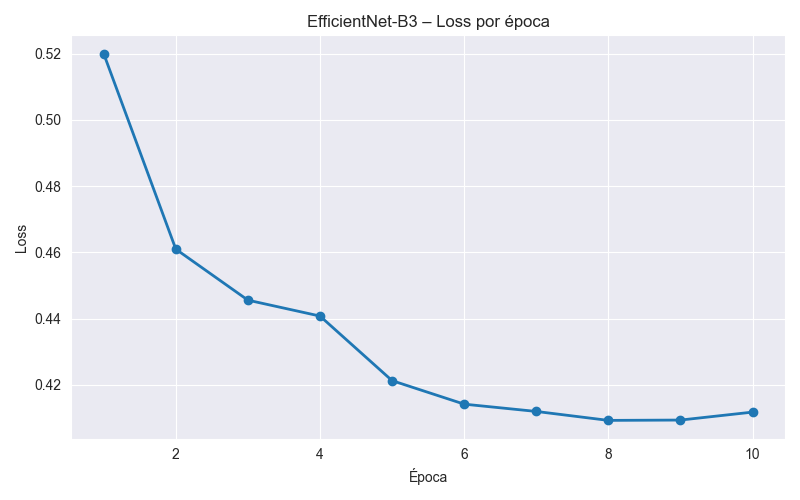
\includegraphics[width=\textwidth]{images/efficientnetb3_loss_curve.png}
        \caption{Pèrdua}
    \end{subfigure}
    \hfill
    \begin{subfigure}[b]{0.48\textwidth}
        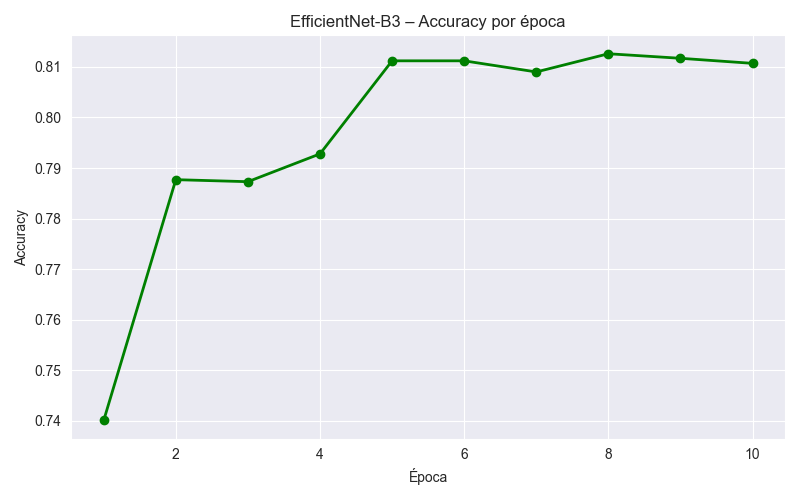
\includegraphics[width=\textwidth]{images/efficientnetb3_accuracy_curve.png}
        \caption{Precisió}
    \end{subfigure}

    \caption{Corbes d’entrenament del model EfficientNet-B3.}
    \label{fig:efficientnetb3_training}
\end{figure}

Tot i que EfficientNet-B3 millora lleugerament EfficientNet-B0 en precisió de la classe
positiva, la seva \textit{accuracy} global va resultar una mica inferior.

\subsection{Avaluació sobre el Conjunt de Test}

El rendiment final del model sobre el conjunt de test va ser:

\[
\text{Accuracy}_{test} = 0.8239.
\]

El \textit{classification report} obtingut va ser:

\begin{table}[h!]
\centering
\begin{tabular}{l|c|c|c|c}
\hline
\textbf{Classe} & \textbf{Precision} & \textbf{Recall} & \textbf{F1-score} & \textbf{Support} \\
\hline
0 & 0.8358 & 0.9317 & 0.8811 & 732 \\
1 & 0.7817 & 0.5719 & 0.6605 & 313 \\
\hline
\textbf{Accuracy} & \multicolumn{4}{c}{0.8239} \\
\textbf{Macro avg} & 0.8087 & 0.7518 & 0.7708 & 1045 \\
\textbf{Weighted avg} & 0.8196 & 0.8239 & 0.8151 & 1045 \\
\hline
\end{tabular}
\caption{Classification report del model EfficientNet-B3.}
\label{tab:efficientnetb3_report}
\end{table}

La matriu de confusió obtinguda va ser:

\begin{figure}[H]
    \centering
    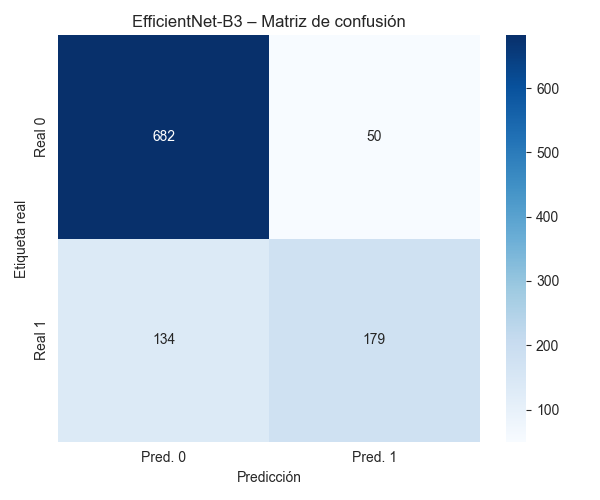
\includegraphics[width=0.65\textwidth]{images/efficientnetb3_confusion_matrix.png}
    \caption{Matriu de confusió obtinguda pel model EfficientNet-B3 sobre el conjunt de test.}
    \label{fig:efficientnetb3_cm}
\end{figure}

la qual cosa indica que el model manté un excel·lent rendiment en la classe negativa, però
redueix la sensibilitat per a la classe positiva respecte a EfficientNet-B0.

\subsection{Anàlisi del Model}

El comportament d’EfficientNet-B3 mostra:

\begin{itemize}
    \item Molt bona precisió per a la classe negativa (93.17\%),
    \item Reducció notable del \textit{recall} per a la classe positiva (57.19\%),
    \item F1-score de la classe positiva inferior al obtingut per EfficientNet-B0,
    \item \textit{Accuracy} global del 82.39\%, menor que l’obtinguda amb models més lleugers.
\end{itemize}

Això suggereix que, malgrat la seva major capacitat, EfficientNet-B3 no generalitza millor que
EfficientNet-B0 sobre aquest dataset específic. Una possible explicació és que el
dataset relativament petit afavoreix models amb menor complexitat, o que les capes
superiors d’EfficientNet-B3 retenen representacions massa específiques d’ImageNet.


\section{Model 6: Transfer Learning amb DenseNet-169}

DenseNet-169 és una versió més profunda de la família DenseNet, caracteritzada per les seves
connexions denses entre capes que faciliten la propagació del gradient i la reutilització
de característiques. A causa del seu elevat poder representacional, es va avaluar com a possible
millora respecte a DenseNet-121 i EfficientNet-B0, analitzant el seu rendiment sobre el
dataset NODE21.

\subsection{Preparació del Dataset}

El preprocessament de les imatges va ser idèntic al que es va emprar en els models anteriors.
Totes les radiografies en format MHA es van normalitzar en el rang $[0,1]$, es van
redimensionar a $224 \times 224$, i es va replicar el canal únic en tres canals RGB per
poder utilitzar pesos preentrenats a ImageNet:

\begin{lstlisting}[style=mypython]
img = img_np.astype(np.float32)
img = (img - img.min()) / (img.max() - img.min())
img = cv2.resize(img, (224,224))
img = np.expand_dims(img, axis=0)
img = np.repeat(img, 3, axis=0)
\end{lstlisting}

El conjunt final va quedar distribuït en:

\[
\text{Train: }4179, \qquad
\text{Test: }1045, \qquad
\text{Total vàlides: }5224.
\]

\subsection{Arquitectura i Transfer Learning}

El model es va inicialitzar amb \texttt{DenseNet169\_Weights.IMAGENET1K\_V1}. Totes les capes
de l’extractor de característiques es van congelar i únicament es va reentrenar la capa final
del classificador:

\begin{lstlisting}[style=mypython]
model = models.densenet169(
    weights=models.DenseNet169_Weights.IMAGENET1K_V1
)

for param in model.parameters():
    param.requires_grad = False

num_features = model.classifier.in_features
model.classifier = nn.Linear(num_features, 2)
\end{lstlisting}

Aquest enfocament redueix el risc de sobreajust i permet adaptar la xarxa a la classificació
binària de nòduls pulmonars.

\subsection{Entrenament}

L’entrenament es va realitzar durant 10 èpoques emprant:

\begin{itemize}
    \item Optimitzador Adam amb \textit{learning rate} $1 \times 10^{-3}$,
    \item Funció de pèrdua CrossEntropy,
    \item Batch size de 32,
    \item Execució en GPU.
\end{itemize}

L’evolució de l’entrenament es resumeix a la Taula~\ref{tab:densenet169_training}.

\begin{table}[h!]
\centering
\begin{tabular}{c|c|c}
\hline
\textbf{Època} & \textbf{Loss} & \textbf{Accuracy} \\
\hline
1  & 0.4924 & 0.7600 \\
2  & 0.3933 & 0.8227 \\
3  & 0.3617 & 0.8454 \\
4  & 0.3407 & 0.8564 \\
5  & 0.3261 & 0.8610 \\
6  & 0.3267 & 0.8615 \\
7  & 0.3024 & 0.8737 \\
8  & 0.2981 & 0.8720 \\
9  & 0.2956 & 0.8753 \\
10 & 0.2891 & 0.8777 \\
\hline
\end{tabular}
\caption{Pèrdua i precisió durant l’entrenament de DenseNet-169.}
\label{tab:densenet169_training}
\end{table}

\begin{figure}[H]
    \centering
    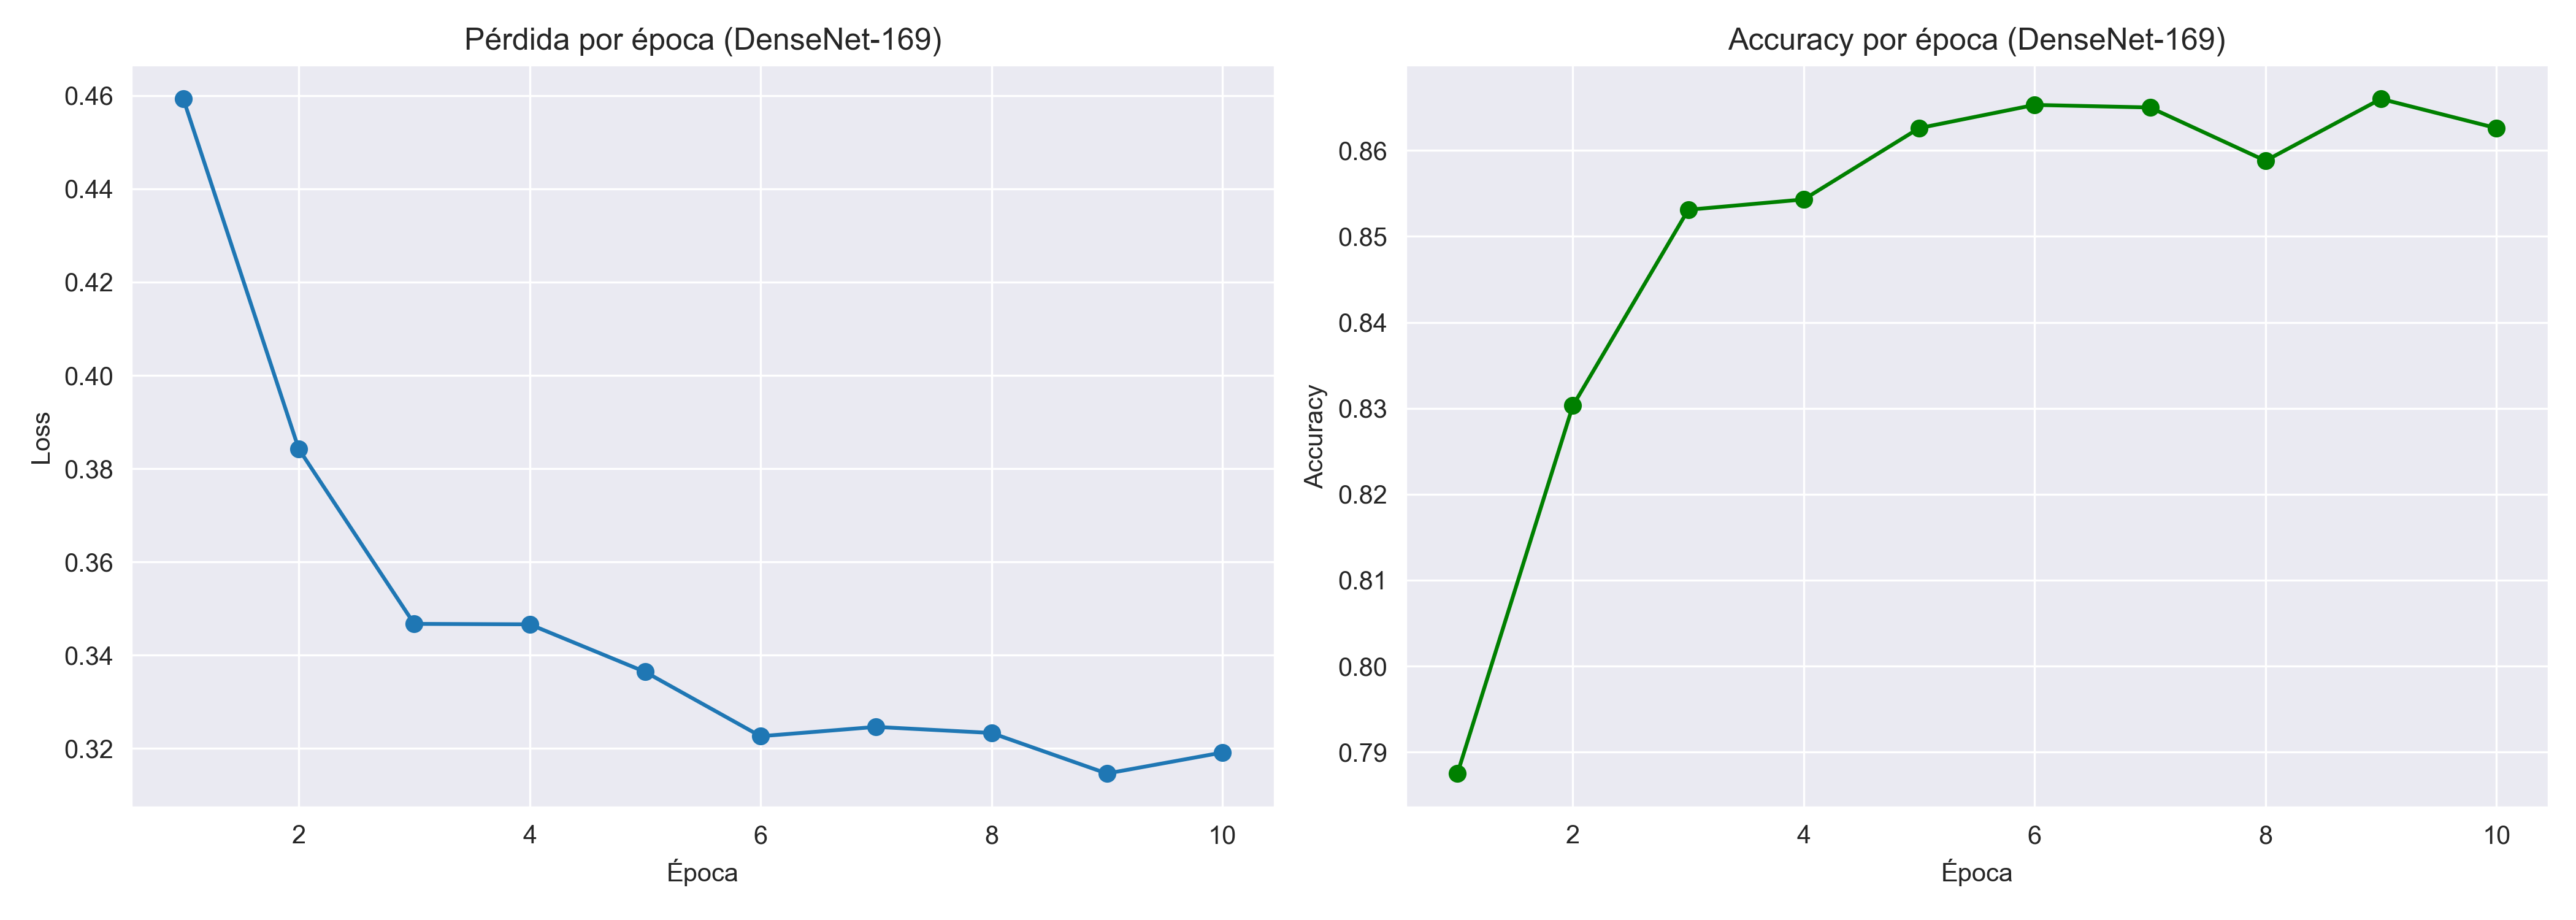
\includegraphics[width=0.90\textwidth]{images/densenet169_training_curves.png}
    \caption{Evolució de la pèrdua (\textit{loss}) i de la precisió (\textit{accuracy}) durant l’entrenament del model DenseNet-169.}
    \label{fig:densenet169_training}
\end{figure}

El model mostra una millora contínua, assolint la major precisió d’entrenament
entre tots els models avaluats fins a aquest punt.

\subsection{Avaluació sobre el Conjunt de Test}

En avaluar el model sobre el 20\% de dades reservades, es va obtenir:

\[
\text{Accuracy}_{test} = 0.8536.
\]

El \textit{classification report} va ser el següent:

\begin{table}[h!]
\centering
\begin{tabular}{l|c|c|c|c}
\hline
\textbf{Classe} & \textbf{Precision} & \textbf{Recall} & \textbf{F1-score} & \textbf{Support} \\
\hline
0 & 0.8824 & 0.9126 & 0.8972 & 732 \\
1 & 0.7778 & 0.7157 & 0.7454 & 313 \\
\hline
\textbf{Accuracy} & \multicolumn{4}{c}{0.8536} \\
\textbf{Macro avg} & 0.8301 & 0.8141 & 0.8213 & 1045 \\
\textbf{Weighted avg} & 0.8511 & 0.8536 & 0.8518 & 1045 \\
\hline
\end{tabular}
\caption{Classification report del model DenseNet-169.}
\label{tab:densenet169_report}
\end{table}

La matriu de confusió obtinguda va ser:

\begin{figure}[H]
    \centering
    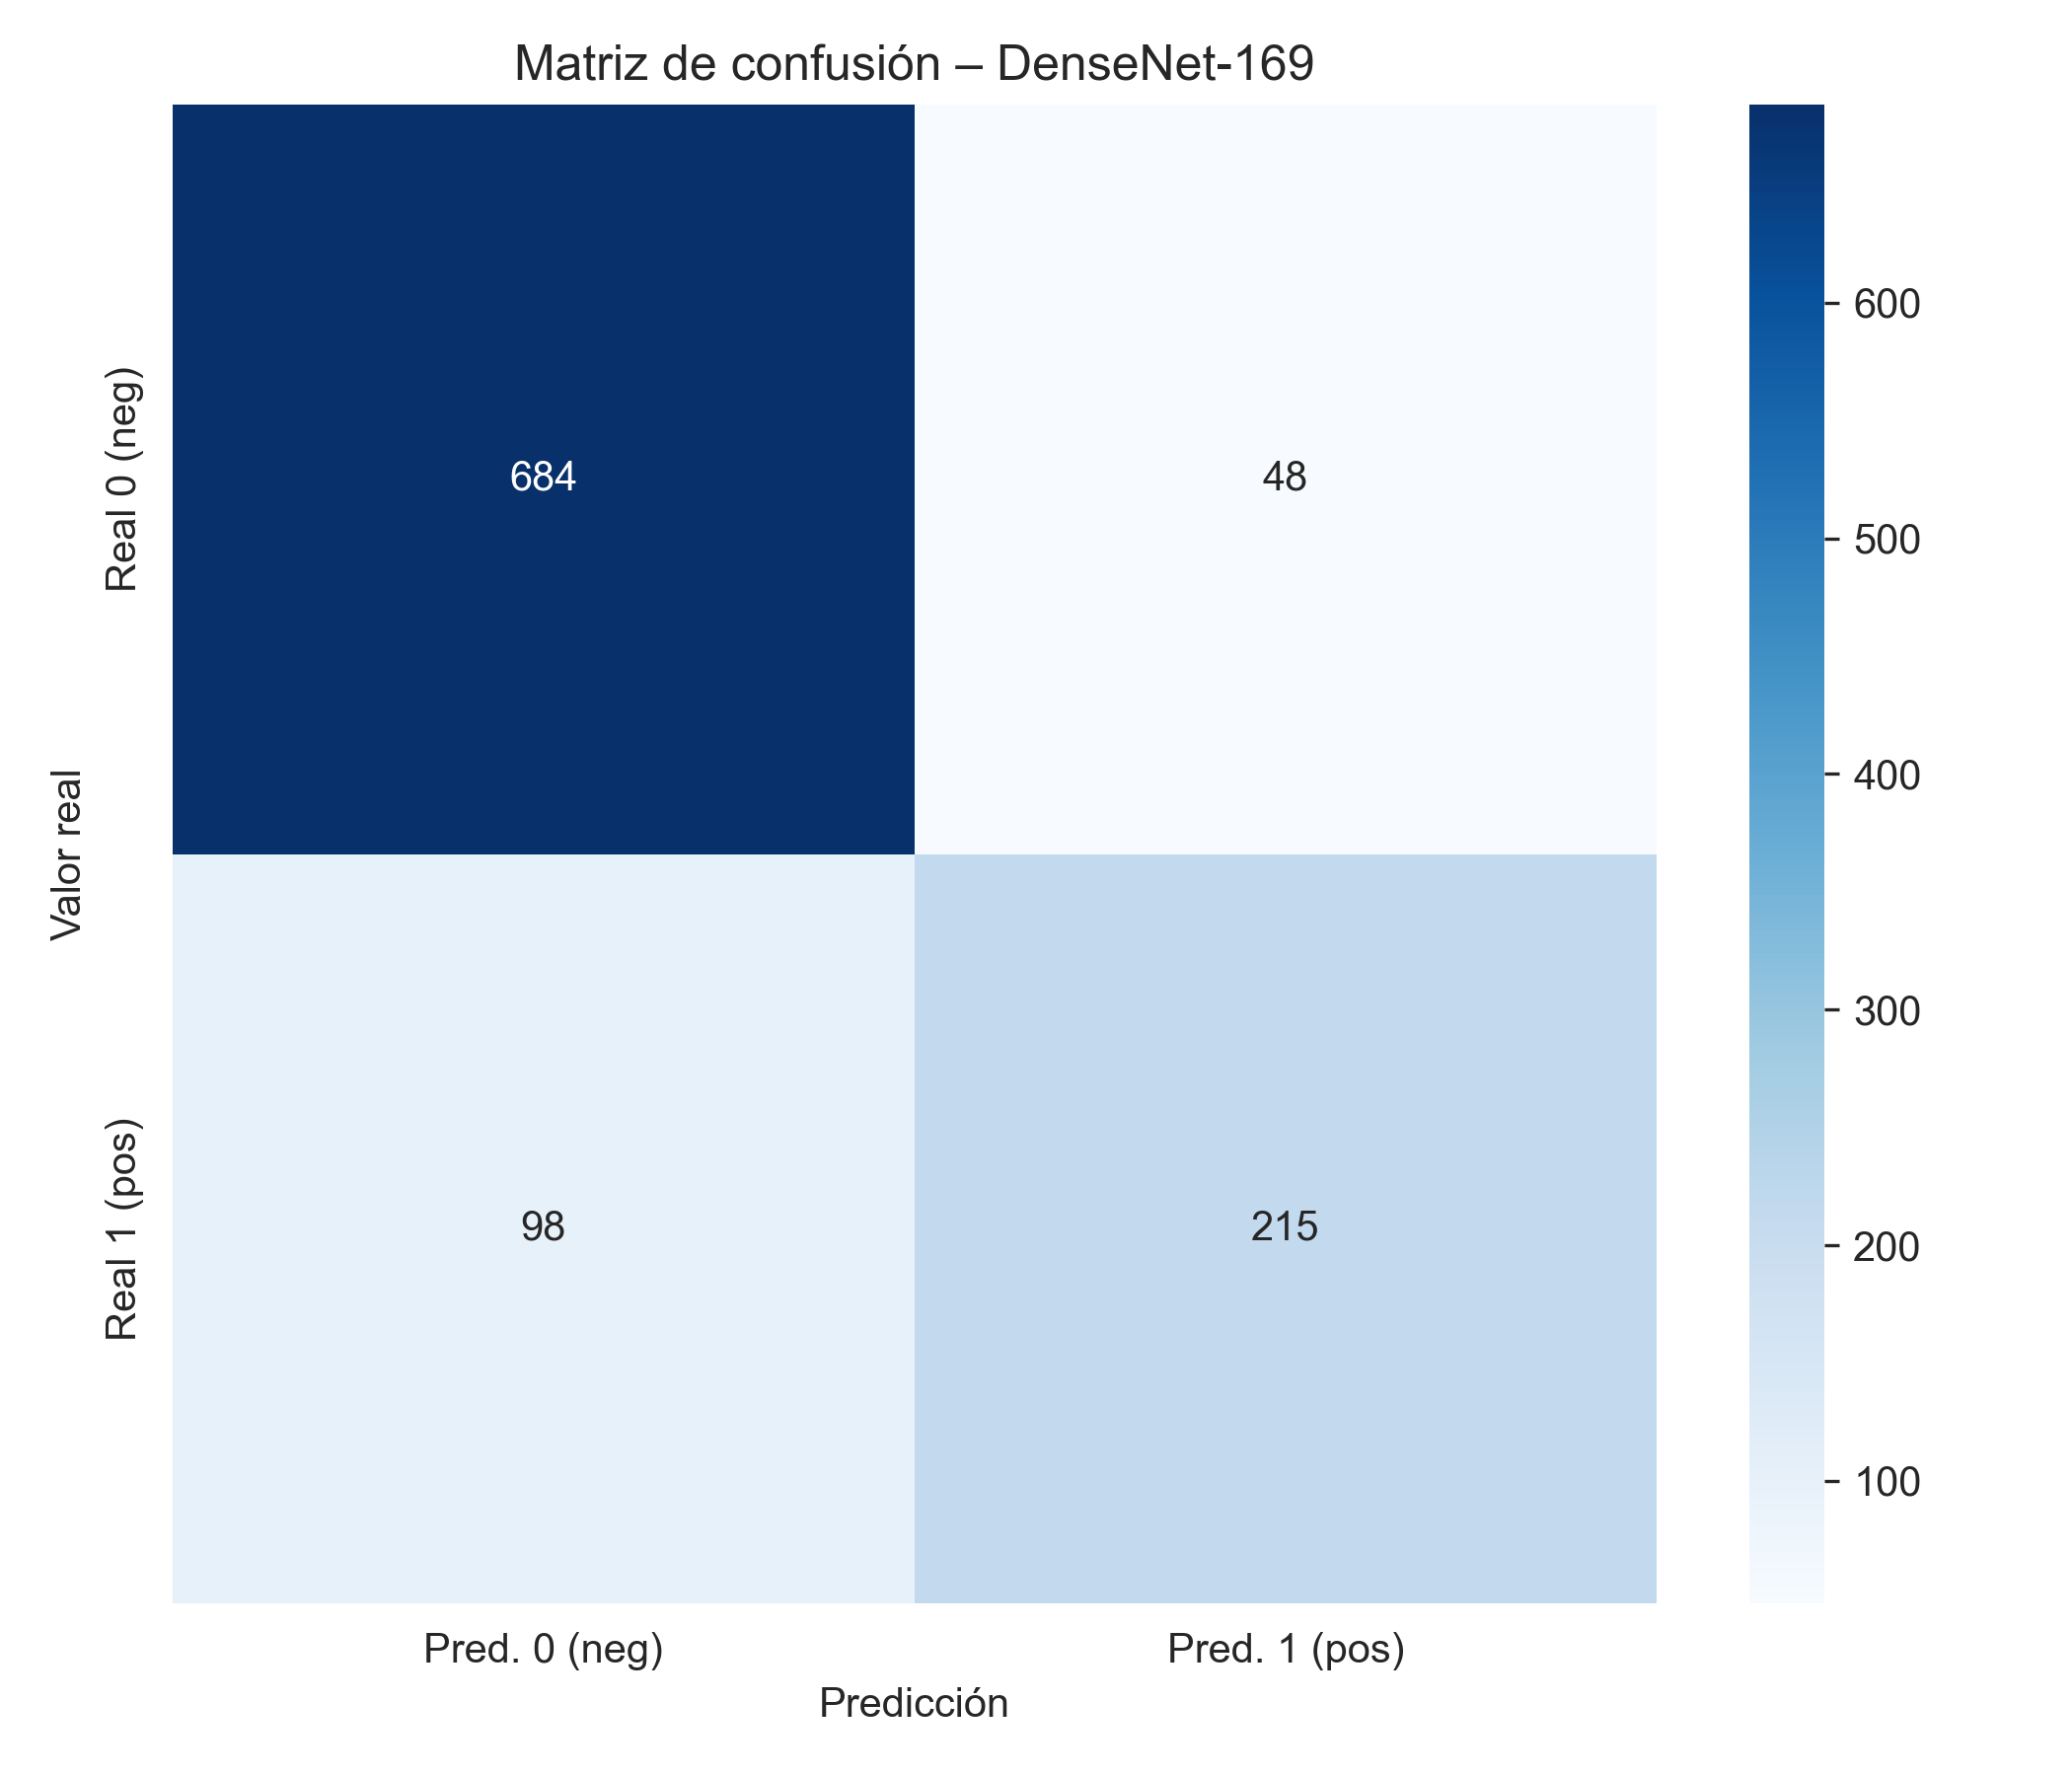
\includegraphics[width=0.65\textwidth]{images/densenet169_confusion_matrix.png}
    \caption{Matriu de confusió del model DenseNet-169 avaluat sobre el conjunt de test.}
    \label{fig:densenet169_confusion}
\end{figure}

la qual cosa reflecteix un bon equilibri entre sensibilitat i precisió, especialment en la
detecció de la classe positiva.

\subsection{Anàlisi del Model}

DenseNet-169 ofereix un rendiment competitiu, situant-se lleugerament per davall de
EfficientNet-B0 però superant ResNet18 i la CNN entrenada des de zero. Les seves principals
característiques són:

\begin{itemize}
    \item Excel·lent \textit{recall} per a la classe negativa (91.26\%).
    \item Bon rendiment en la classe positiva, amb un F1-score de 0.7454.
    \item Entrenament estable i sense signes de sobreajust sever.
\end{itemize}

El seu comportament confirma que arquitectures més profundes amb connexions denses poden
capturar millor l’estructura dels nòduls, tot i que la seva capacitat no arriba a superar
EfficientNet en aquest experiment.


\section{Resultados de la Comparación de Modelos}

La Figura~\ref{fig:comparativa_modelos} resume el rendimiento de los seis modelos evaluados en esta primera fase del proyecto: una CNN entrenada desde cero, ResNet18, DenseNet121, EfficientNet-B0, EfficientNet-B3 y DenseNet169. Los resultados muestran una tendencia clara: las arquitecturas profundas preentrenadas ofrecen un rendimiento significativamente superior al del modelo construido desde cero, lo cual era esperable dada la complejidad del problema y el tamaño reducido del conjunto de datos.

\begin{figure}[H]
    \centering
    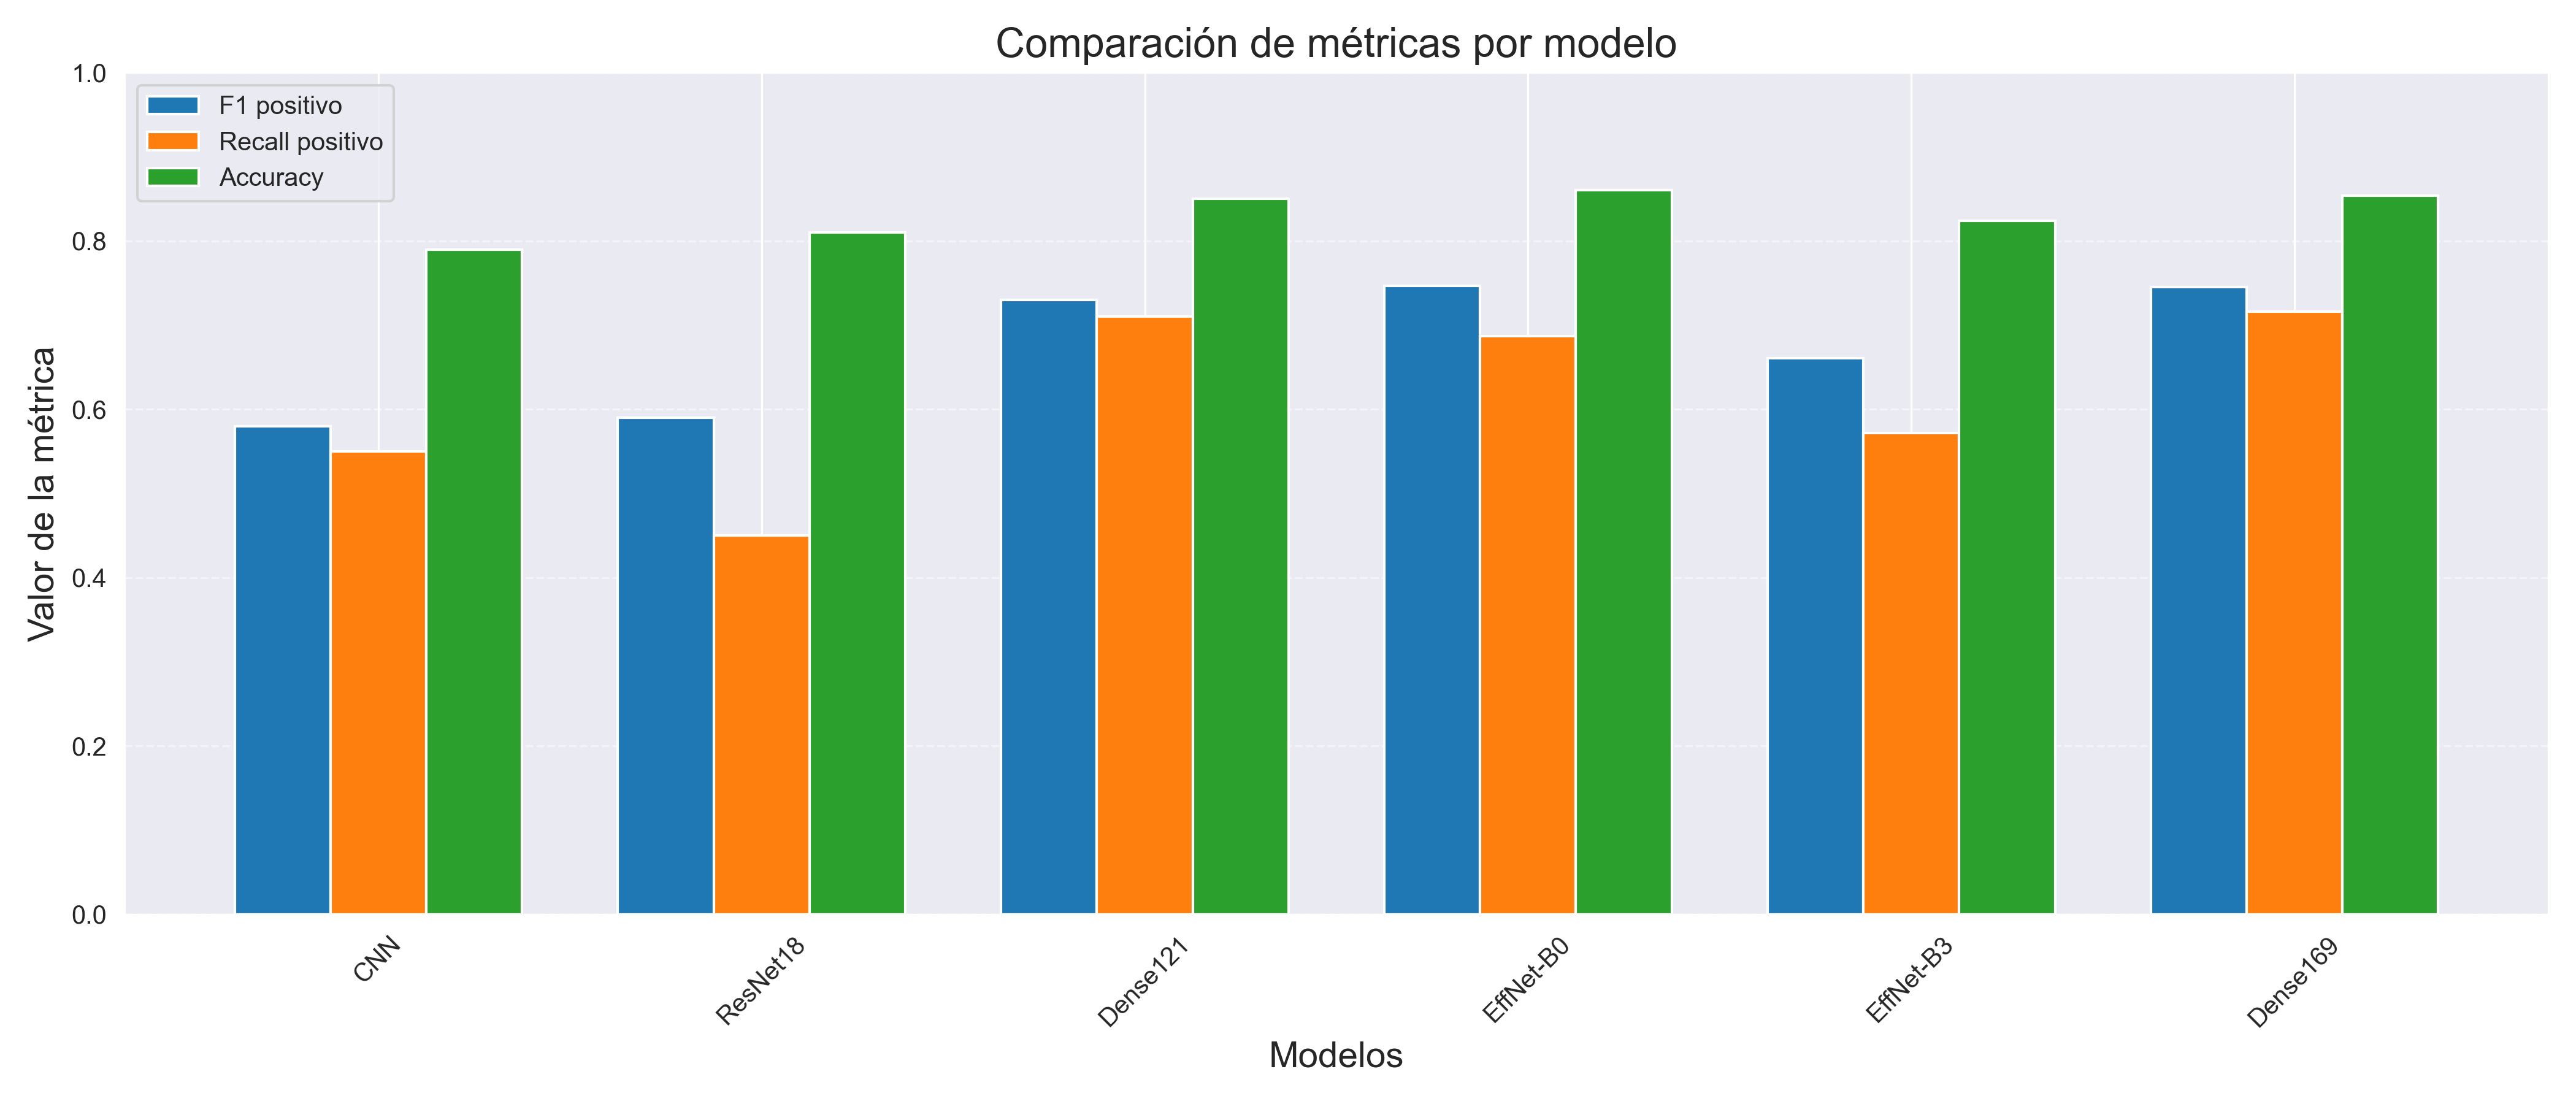
\includegraphics[width=0.95\textwidth]{images/comparacion_metrica_por_modelo_clasificacion.png}
    \caption{
        Comparación de las métricas principales (\textit{F1-score} positivo, 
        \textit{recall} positivo y \textit{accuracy}) para los seis modelos 
        evaluados: CNN entrenada desde cero, ResNet18, DenseNet121, 
        EfficientNet-B0, EfficientNet-B3 y DenseNet169. 
        La gráfica permite observar el impacto del \textit{transfer learning} 
        y la superioridad de las arquitecturas profundas preentrenadas frente 
        al modelo construido desde cero.
    }
    \label{fig:comparativa_modelos}
\end{figure}


Entre los modelos evaluados, \textbf{EfficientNet-B0} y \textbf{DenseNet169} destacan como las alternativas más equilibradas, alcanzando valores de \textit{F1-Score} cercanos a 0.75 y precisiones globales superiores al 0.85. Esto representa una mejora sustancial respecto a enfoques previos.

Sin embargo, el análisis del \textit{recall} positivo ---la métrica más crítica en un problema clínico donde los falsos negativos deben minimizarse--- revela una limitación importante: ninguno de los modelos supera el valor de 0.72, y algunos descienden incluso por debajo del 0.60. Esto indica que, aunque los modelos clasifican correctamente una proporción elevada de radiografías normales, siguen \textbf{fallando en una fracción relevante de los casos positivos}, lo cual es crítico en un contexto de cribado de nódulos pulmonares.

A partir de este análisis pueden extraerse dos conclusiones principales:

\begin{enumerate}
    \item El \textit{transfer learning} es claramente superior al entrenamiento desde cero en radiología, especialmente en datasets con señales sutiles y tamaño limitado.
    \item Incluso los mejores modelos aún no capturan de forma suficiente la complejidad morfológica del nódulo pulmonar, especialmente su variabilidad en tamaño y forma.
\end{enumerate}

En consecuencia, y siguiendo el enunciado de la práctica, planteamos avanzar hacia una fase de \textbf{innovación del modelo}, con el objetivo de ayudar a la red de la misma forma que lo hace un radiólogo humano. Para ello, se explorarán estrategias que introduzcan información adicional o transformaciones específicas, tales como:

\begin{itemize}
    \item realce de bordes y estructuras pulmonares relevantes,
    \item generación de canales adicionales que destaquen patrones nodulares,
    \item normalización anatómica inspirada en la práctica clínica,
    \item incorporación de mapas o máscaras que guíen la atención del modelo.
\end{itemize}

Este cambio de enfoque busca no solo mejorar el rendimiento global, sino también reducir de forma drástica los falsos negativos, que representan actualmente el principal cuello de botella en el proceso de clasificación. La siguiente sección desarrolla esta nueva propuesta metodológica.

\section{Fase d'Innovació: Motivació, Plantejament i Objectius}

Després d'haver avaluat diverses arquitectures estàndard de classificació ---incloent
CNNs entrenades des de zero, ResNet18, DenseNet121, DenseNet169 i diferents variants
d'EfficientNet--- els resultats mostren de manera consistent una limitació important:
tot i que la \textit{accuracy} global dels models és elevada, el \textbf{recall de la
classe positiva (nòduls pulmonars)} es manté sistemàticament per davall del nivell
desitjat per a un sistema d'ajuda al diagnòstic radiològic.

Aquesta observació és coherent amb el comportament habitual dels models
\textit{off-the-shelf} en imatge mèdica: els senyals corresponents a lesions petites,
difuses o de baix contrast sovint són difícils d'aprendre quan el model només rep la
imatge original. En canvi, els professionals radiòlegs no basen la seva interpretació en
una sola ``versió'' de la imatge, sinó en un \textit{processament visual seqüencial} que
inclou contrast local, contorns, patrons de textura i microdetall.

Aquest fet va motivar l'inici d'una fase d'innovació amb l'objectiu d'\textbf{apropar el
pipeline computacional al procés de lectura radiològica humana}. En concret, es van
plantejar dues línies principals de millora:

\begin{enumerate}
    \item \textbf{Codificació multicanal de la radiografia}, incorporant transformacions
    específiques que reforcen informació clínica rellevant: normalització, CLAHE,
    detecció de contorns (Canny) i filtres d'enfocament (Unsharp Mask).
    \item \textbf{Reequilibrat del conjunt de dades mitjançant augmentació dirigida},
    aplicant transformacions plausibles només sobre la classe minoritària per evitar
    biaixos i millorar la sensibilitat del model.
\end{enumerate}

Ambdós enfocaments tenen una motivació clara: proporcionar al model una representació més
rica i informativa de la imatge, imitant de manera computacional el tipus de cues
diagnòstiques que utilitzen els radiòlegs. Aquesta aproximació no només millora la
separabilitat de les classes, sinó que també permet que arquitectures com EfficientNet-B0
aproveitin la seva capacitat per integrar informació heterogènia d'una manera més
eficient.

Els resultats obtinguts després de la incorporació d’aquests elements mostren una
millora notable respecte dels models originals, situant la nova versió del model en un
règim de rendiment considerablement superior.

A continuació, es presenta detalladament \textbf{el conjunt de tècniques específiques que
s’han introduït per millorar significativament el rendiment del classificador}, així com
els resultats experimentals associats a cadascuna d’elles.

Finalment, cal destacar que en fases posteriors del projecte es preveu la realització
d’un \textbf{estudi d’ablació complet}, amb l’objectiu d’analitzar de manera rigorosa la
contribució individual de cada component (canals afegits, estratègies d’augmentació,
reequilibrat del dataset i arquitectura emprada). Aquest estudi permetrà establir una
base quantitativa sòlida per identificar quines parts del pipeline són realment
crítiques i quines tenen un impacte secundari.


\subsection{Augmentació del Dataset per a Classificació}

Per tal de millorar el rendiment dels models de classificació i compensar el fort
desbalanceig present en el conjunt de dades original del repte NODE21, es va aplicar una
estratègia d'\textbf{augmentació orientada exclusivament a la tasca de classificació},
sense utilitzar en cap moment les \textit{bounding boxes} disponibles al dataset
original.

Aquesta decisió és important: l'objectiu d’aquesta fase del projecte no és entrenar un
model de detecció, sinó únicament un \textit{classificador binari} que determini la
presència o absència d’un nòdul. Per tant, les noves imatges augmentades podien
transformar-se lliurement sense preocupar-se de desplaçar, deformar o invalidar cap
anotació espacial.

\subsubsection*{Augmentació aplicada exclusivament a la classe positiva}

El conjunt original presenta una distribució molt desequilibrada, amb una proporció de
negatius molt superior als positius. Per evitar que els models aprenguin un biaix cap a
la classe majoritària, es va aplicar augmentació només sobre les imatges etiquetades com
a nòduls. Aquest augment dirigits permet:

\begin{itemize}
    \item incrementar el nombre efectiu de mostres positives,
    \item millorar la robustesa del model davant variabilitat real,
    \item reduir el risc d’overfitting en un conjunt inicialment petit.
\end{itemize}

Les transformacions aplicades, totes elles considerades segures en imatge mèdica perquè
no alteren la morfologia essencial del nòdul, varen ser les següents:

\begin{itemize}
    \item \textbf{Soroll gaussià suau}: simula variabilitat d’adquisició.
    \item \textbf{Blur gaussià lleu}: afebleix detalls i obliga el model a generalitzar.
    \item \textbf{Correcció gamma}: modifica el rang tonal i il·luminació.
    \item \textbf{Ajust de brillantor}: exposicions lleugerament més altes o baixes.
    \item \textbf{Ajust de contrast}: millores o reduccions controlades del contrast global.
    \item \textbf{Filtre \emph{sharpen}}: reforç dels contorns.
    \item \textbf{CLAHE}: millora el contrast local en zones pulmonars amb poca definició.
    \item \textbf{Petites distorsions afins}: simulen variacions d’adquisició entre equips.
\end{itemize}

És important remarcar que es van evitar transformacions que poguessin alterar la
geometria del pulmó (com rotacions fortes o canvis d’escala), ja que els nòduls són
estructures petites i qualsevol deformació excessiva podria generar patrons artificials.

\subsubsection*{Resultat del procés d’augmentació}

Abans de l’augmentació, la distribució del dataset era:

\[
\text{positius} = 1476, \qquad \text{negatius} = 3748.
\]

Per equilibrar ambdues classes es varen generar:

\[
3748 - 1476 = 2272 \text{ imatges augmentades}.
\]

Aquestes imatges es van guardar com a nous fitxers independents i incorporades al
\textit{metadata} general per formar un conjunt equilibrat final.

La distribució després del procés és:

\[
\text{positius} = 3748, \qquad \text{negatius} = 3748.
\]

Així, s’obté un dataset total de 7496 mostres, perfectament balancejat i adequat per
entrenar classificadors moderns sense introduir biaixos cap a la classe majoritària.

\subsubsection*{Beneficis observats}

L’augmentació dirigida ha tingut tres efectes clau:

\begin{enumerate}
    \item \textbf{Reducció del biaix de classificació}: el model deixa d'aprendre a predir
    sempre la classe negativa.
    \item \textbf{Millora del recall positiu}: increment substancial en la sensibilitat del
    model envers nòduls reals.
    \item \textbf{Generalització millorada}: els models entrenats amb augmentació mostren
    menys variabilitat entre entrenament i validació.
\end{enumerate}

Aquest dataset augmentat i balancejat constitueix la base sobre la qual es construiran les
fases següents del projecte, incloent la codificació multicanal i la millora progressiva
del model de classificació.


\subsection{Codificació Multicanal: Disseny i Fonament Teòric}

La innovació principal consisteix a construir una representació multicanal de cada
radiografia, afegint-hi informació derivada de transformacions clíniques rellevants.
Aquest enfocament busca imitar la manera com un radiòleg analitza la imatge, i permet al
model disposar de cues visuals addicionals que reforcen patrons morfològics de difícil
detecció.

Els tres canals incorporats en aquesta fase són:

\begin{enumerate}
    \item \textbf{Canal 1: Imatge original normalitzada}.  
    És el punt de partida sobre el qual es basa qualsevol procés d’anàlisi. Conté la
    distribució d’intensitats real i el context anatòmic complet.

    \item \textbf{Canal 2: CLAHE (Contrast Limited Adaptive Histogram Equalization)}.  
    Aquesta tècnica, habitual en radiologia, realça selectivament zones de baix contrast,
    especialment útil en lesions pulmonars poc definides. Proporciona al model una visió
    ``optimitzada'' de la textura i del gradient local de la imatge, que facilita la
    separació de teixits.

    \item \textbf{Canal 3: Detecció de contorns Canny}.  
    Aquest canal reforça les fronteres estructurals, com ara la perifèria del nòdul. Els
    contorns són crucials per diferenciar masses nodulars de patrons pulmonars normals.
    Afegir aquest canal permet al model identificar discontinuïtats geomètriques que no
    són evidents en la imatge original.
\end{enumerate}

\begin{figure}[H]
    \centering
    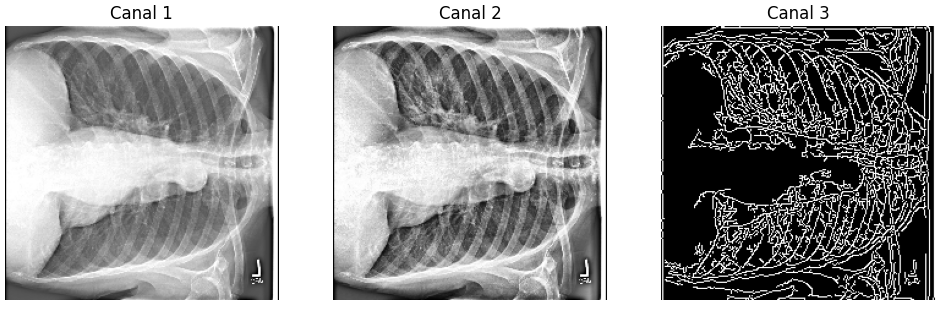
\includegraphics[width=0.95\textwidth]{images/rx_3_capas.png}
    \caption{Visualización de los tres canales generados para cada radiografía: 
    (1) imagen original normalizada, 
    (2) imagen con realce de contraste mediante CLAHE, 
    (3) mapa de bordes obtenido con el algoritmo Canny. 
    Esta representación multicanal permite que la red neuronal disponga de información complementaria sobre intensidad, contraste y estructura geométrica del nódulo.}
    \label{fig:rx_3_capas}
\end{figure}


La combinació d’aquests tres canals genera una representació de dimensió
\((3 \times 224 \times 224)\) que encapsula:

\begin{itemize}
    \item intensitat global (canal original),
    \item textura i contrast local (CLAHE),
    \item morfologia i estructura del contorn (Canny).
\end{itemize}

Des del punt de vista teòric, això equival a definir un espai de característiques molt
més discriminatiu que aquell que pot oferir una sola imatge de RX. Models com
EfficientNet-B0, dissenyats per integrar informació multi-escala i multi-canal, són
especialment adequats per explotar aquesta riquesa de senyal.



\subsection{Descripció General del Pipeline de Processament i Classificació}

Abans de presentar en detall la fase d’innovació i els resultats obtinguts, es descriu de
manera general l’estructura del codi implementat. L’objectiu és proporcionar una visió
global del funcionament del pipeline, destacant els components principals i el rol de
cada un dins del procés complet de classificació.

El codi es divideix en diversos blocs funcionals, cadascun dels quals s’encarrega d’una
part concreta del flux de treball: càrrega de dades, preprocessament, construcció del
dataset, augmentació, definició dels models i preparació dels \textit{dataloaders} per a
l’entrenament.

\subsubsection{Càrrega inicial de llibreries i configuració del dispositiu}

El primer bloc importa totes les llibreries necessàries per gestionar tensors
(PyTorch), processar imatges (OpenCV), carregar fitxers MHA (OpenCXR), generar gràfics
(Matplotlib) i avaluar els models (Scikit-Learn). També es detecta automàticament si hi
ha GPU disponible:

\begin{lstlisting}[style=mypython]
device = torch.device("cuda" if torch.cuda.is_available() else "cpu")
print("Device:", device)
\]
\end{lstlisting}
Aquest pas assegura que l’execució s’optimitza al màxim segons els recursos disponibles.

\subsubsection{Càrrega del metadata i validació de fitxers}

A continuació, es carrega el fitxer \texttt{metadata.csv}, que conté els noms de les
imatges i les etiquetes (0 = no nòdul, 1 = nòdul). Per evitar errors durant
l’entrenament, es verifica que cada imatge existeixi físicament al directori corresponent
i només es conserven les rutes vàlides.

Aquest filtratge és essencial perquè en els datasets clínics és habitual trobar imatges
que no s’han generat correctament o que han estat movides.

\subsubsection{Augmentació per millorar la variabilitat}

El codi defineix una funció d’augmentació que aplica transformacions lleugeres a la
imatge multicanal:

\begin{itemize}
    \item flips horitzontals,
    \item rotacions suaus,
    \item soroll gaussià controlat.
\end{itemize}

Aquestes transformacions tenen com a objectiu augmentar la robustesa del model i reduir
la dependència d’un patró visual concret del dataset. En aquesta fase, només s’aplica
augmentació durant l’entrenament.

\subsubsection{Construcció del dataset multicanal}

La classe \texttt{CXRClassificationDataset} és el nucli del pipeline. Cada vegada que es
carrega una imatge, es duen a terme aquests passos:

\begin{enumerate}
    \item Lectura del fitxer MHA mitjançant \texttt{read\_file}.
    \item Normalització de la imatge a l’interval \([0,1]\).
    \item Redimensionat a \(224\times224\) píxels.
    \item Generació de tres canals:
    \begin{itemize}
        \item original normalitzada,
        \item CLAHE per realçar contrast local,
        \item contorns Canny.
    \end{itemize}
    \item Conversió a tensor PyTorch.
\end{enumerate}

Aquesta representació multicanal substitueix la imatge d'entrada convencional i dota el
model d’una informació visual molt més rica i diagnòstica.

\subsubsection{Definició del collate function}

La funció \texttt{custom\_collate} elimina mostres incorrectes i apila imatges i etiquetes
en un lot (\textit{batch}). Això evita que imatges corruptes o mal llegides interrompin
l’entrenament.

\subsubsection{Divisió train/test i preparació dels DataLoaders}

El dataset es divideix segons una partició estratificada del 80\% per entrenament i 20\%
per test. Els \textit{dataloaders} associen el dataset amb el sistema de càrrega en
lots, habilitant:

\begin{itemize}
    \item mescla aleatòria (\textit{shuffle}) per entrenament,
    \item lectura eficient amb treballadors paral·lels,
    \item compatibilitat amb GPU.
\end{itemize}

\subsubsection{Entrenament universal del model}

La funció \texttt{train\_model} implementa un bucle d’entrenament genèric amb:

\begin{itemize}
    \item \textbf{CrossEntropyLoss} per classificació binària,
    \item \textbf{Adam} com optimitzador,
    \item càlcul de pèrdua i exactitud per època.
\end{itemize}

Aquesta funció és vàlida per a qualsevol arquitectura PyTorch i és fàcilment escalable.

\subsubsection{Model EfficientNet-B0 multicanal amb dataset balancejat}

Després de definir el pipeline multicanal i generar un \textit{dataset} balancejat mitjançant
\textit{data augmentation} específica sobre la classe positiva, es va avaluar l’ús
d’\textbf{EfficientNet-B0} com a model de classificació final. L’objectiu era comprovar fins a quin punt
la combinació de:

\begin{itemize}
    \item codificació multicanal (original + CLAHE + contorns),
    \item augmentació mèdica,
    \item i balanceig de classes
\end{itemize}

permetia superar de manera clara els resultats obtinguts amb les arquitectures provades en la fase anterior
(CNN simple, ResNet18, DenseNet121, EfficientNet-B0 estàndard, etc.).

\subsubsection{Plantejament del model}

Com a punt de partida s’utilitza \texttt{EfficientNet-B0} preentrenat a ImageNet, carregat des de
\texttt{torchvision.models}. Només es modifica la capa final per adaptar el model a una tasca de
classificació binària (\texttt{label} \(\in \{0,1\}\)):

\begin{lstlisting}[style=mypython]
model = models.efficientnet_b0(
    weights=models.EfficientNet_B0_Weights.IMAGENET1K_V1
)

n = model.classifier[1].in_features
model.classifier[1] = nn.Linear(n, 2)
model = model.to(device)

model = train_model(model, train_loader, test_loader, epochs=5)
evaluate_model(model, test_loader)
\end{lstlisting}

En aquest experiment el model rep com a entrada imatges en format multicanal \((3 \times 224 \times 224)\),
on cada canal correspon a:

\begin{itemize}
    \item Canal 1: radiografia original normalitzada a l’interval \([0,1]\).
    \item Canal 2: imatge amb realç de contrast local mitjançant CLAHE.
    \item Canal 3: mapa de contorns obtingut amb l’operador Canny.
\end{itemize}

Aquest disseny pretén imitar, en certa manera, l’estratègia de lectura d’un radiòleg: primer la informació
d’intensitat global, després el contrast regional i, finalment, l’estructura geomètrica i els contorns del
nòdul.

\subsubsection{Configuració d’entrenament}

L’entrenament es realitza sobre el \textit{metadata} balancejat, on les classes positiva (nòdul) i negativa
(no nòdul) tenen el mateix nombre de mostres, gràcies a un procés previ d’augmentació mèdica aplicada
exclusivament sobre la classe minoritària. La configuració d’entrenament és la següent:

\begin{itemize}
    \item Optimitzador: \textbf{Adam}.
    \item Funció de pèrdua: \textbf{CrossEntropyLoss}.
    \item Nombre d’èpoques: 5.
    \item Mida de \textit{batch}: 32.
    \item Dispositiu: GPU (\texttt{device = 'cuda'}) quan està disponible.
\end{itemize}

La funció genèrica \texttt{train\_model} s’encarrega de gestionar el bucle d’entrenament, calculant la
pèrdua mitjana i l’\textit{accuracy} de train a cada època, mentre que \texttt{evaluate\_model} genera
l’informe de classificació i la matriu de confusió sobre el conjunt de test.

\subsubsection{Evolució de l’entrenament}

La Taula~\ref{tab:effb0_multicanal_train} mostra la pèrdua mitjana i l’\textit{accuracy} d’entrenament
per a cadascuna de les cinc èpoques:

\begin{table}[H]
    \centering
    \caption{Evolució de la pèrdua i l’\textit{accuracy} d’entrenament per al model EfficientNet-B0 multicanal amb dataset balancejat.}
    \label{tab:effb0_multicanal_train}
    \begin{tabular}{c c c}
        \hline
        Època & Loss train & Accuracy train \\
        \hline
        1 & 0.3335 & 0.8500 \\
        2 & 0.1827 & 0.9292 \\
        3 & 0.1435 & 0.9435 \\
        4 & 0.1140 & 0.9610 \\
        5 & 0.1057 & 0.9596 \\
        \hline
    \end{tabular}
\end{table}

\begin{figure}[H]
    \centering
    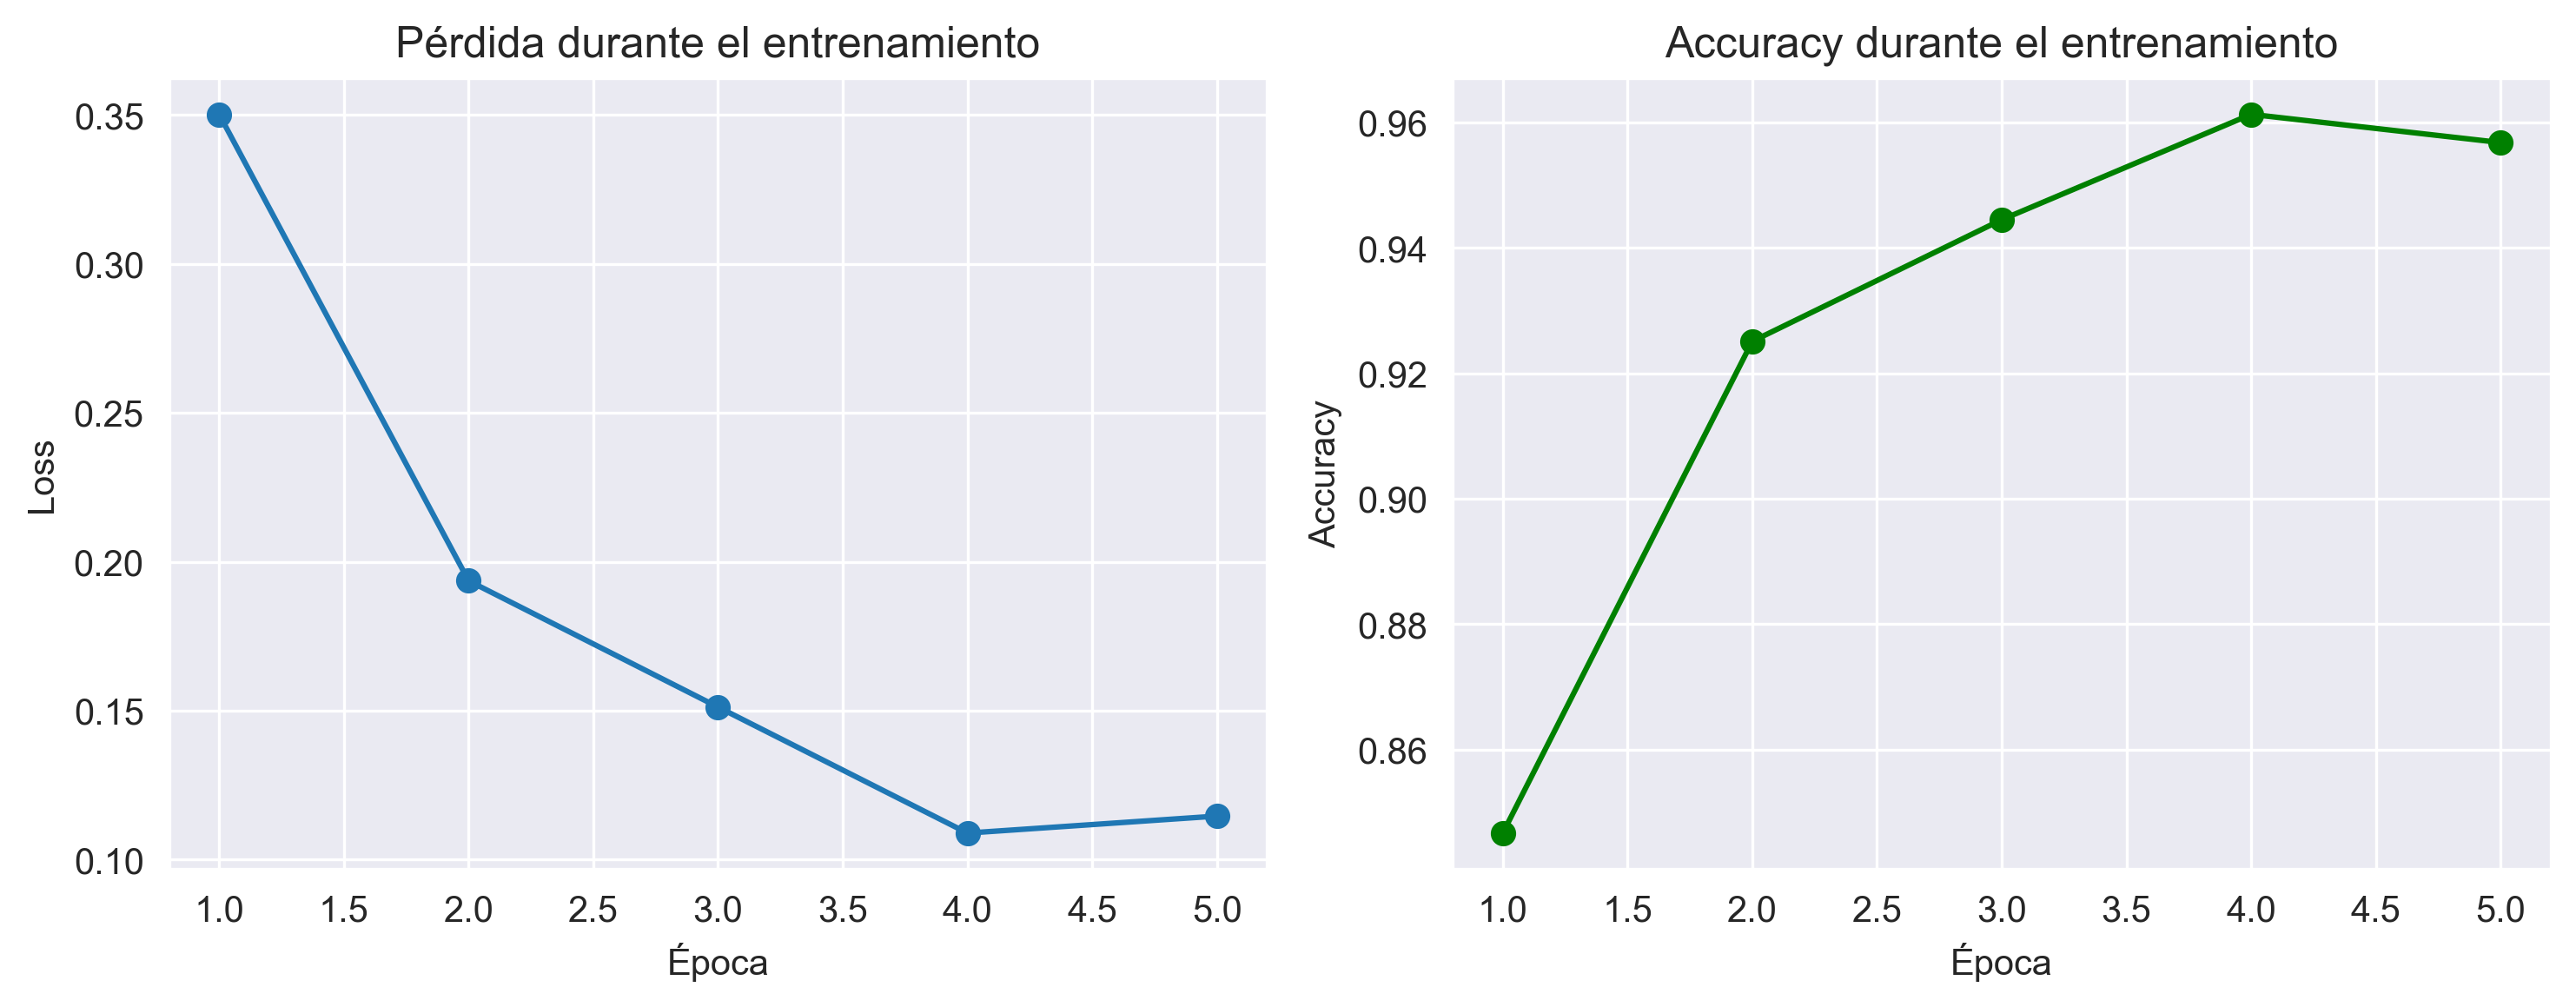
\includegraphics[width=0.95\textwidth]{images/efficientnet_b0_training_curves.png}
    \caption{Evolución de la pérdida (\textit{loss}) y de la precisión (\textit{accuracy}) durante las 5 épocas de entrenamiento del modelo EfficientNet-B0 multicanal. Se observa una reducción progresiva de la pérdida y un incremento estable del rendimiento hasta alcanzar valores próximos al 96\%.}
    \label{fig:effb0_training_curves}
\end{figure}

S’observa una disminució clara de la pèrdua i una millora sostinguda de l’\textit{accuracy}, que
s’estabilitza al voltant de valors pròxims al 96\%. No es detecten signes evidents d’\textit{overfitting}
greu, en part gràcies a l’augmentació i a la diversitat introduïda mitjançant la codificació multicanal.

\subsubsection{Resultats sobre el conjunt de test}

L’avaluació final es realitza sobre un conjunt de test de 1\,045 imatges, obtingut mitjançant
\textit{train/test split} amb llavor fixa (\texttt{random\_state = 42}). L’informe de classificació
resultant és:

\begin{verbatim}
              precision    recall  f1-score   support

           0     0.9875    0.9699    0.9786       732
           1     0.9325    0.9712    0.9515       313

    accuracy                         0.9703      1045
   macro avg     0.9600    0.9706    0.9651      1045
weighted avg     0.9710    0.9703    0.9705      1045
\end{verbatim}

La matriu de confusió associada és:

\begin{figure}[H]
    \centering
    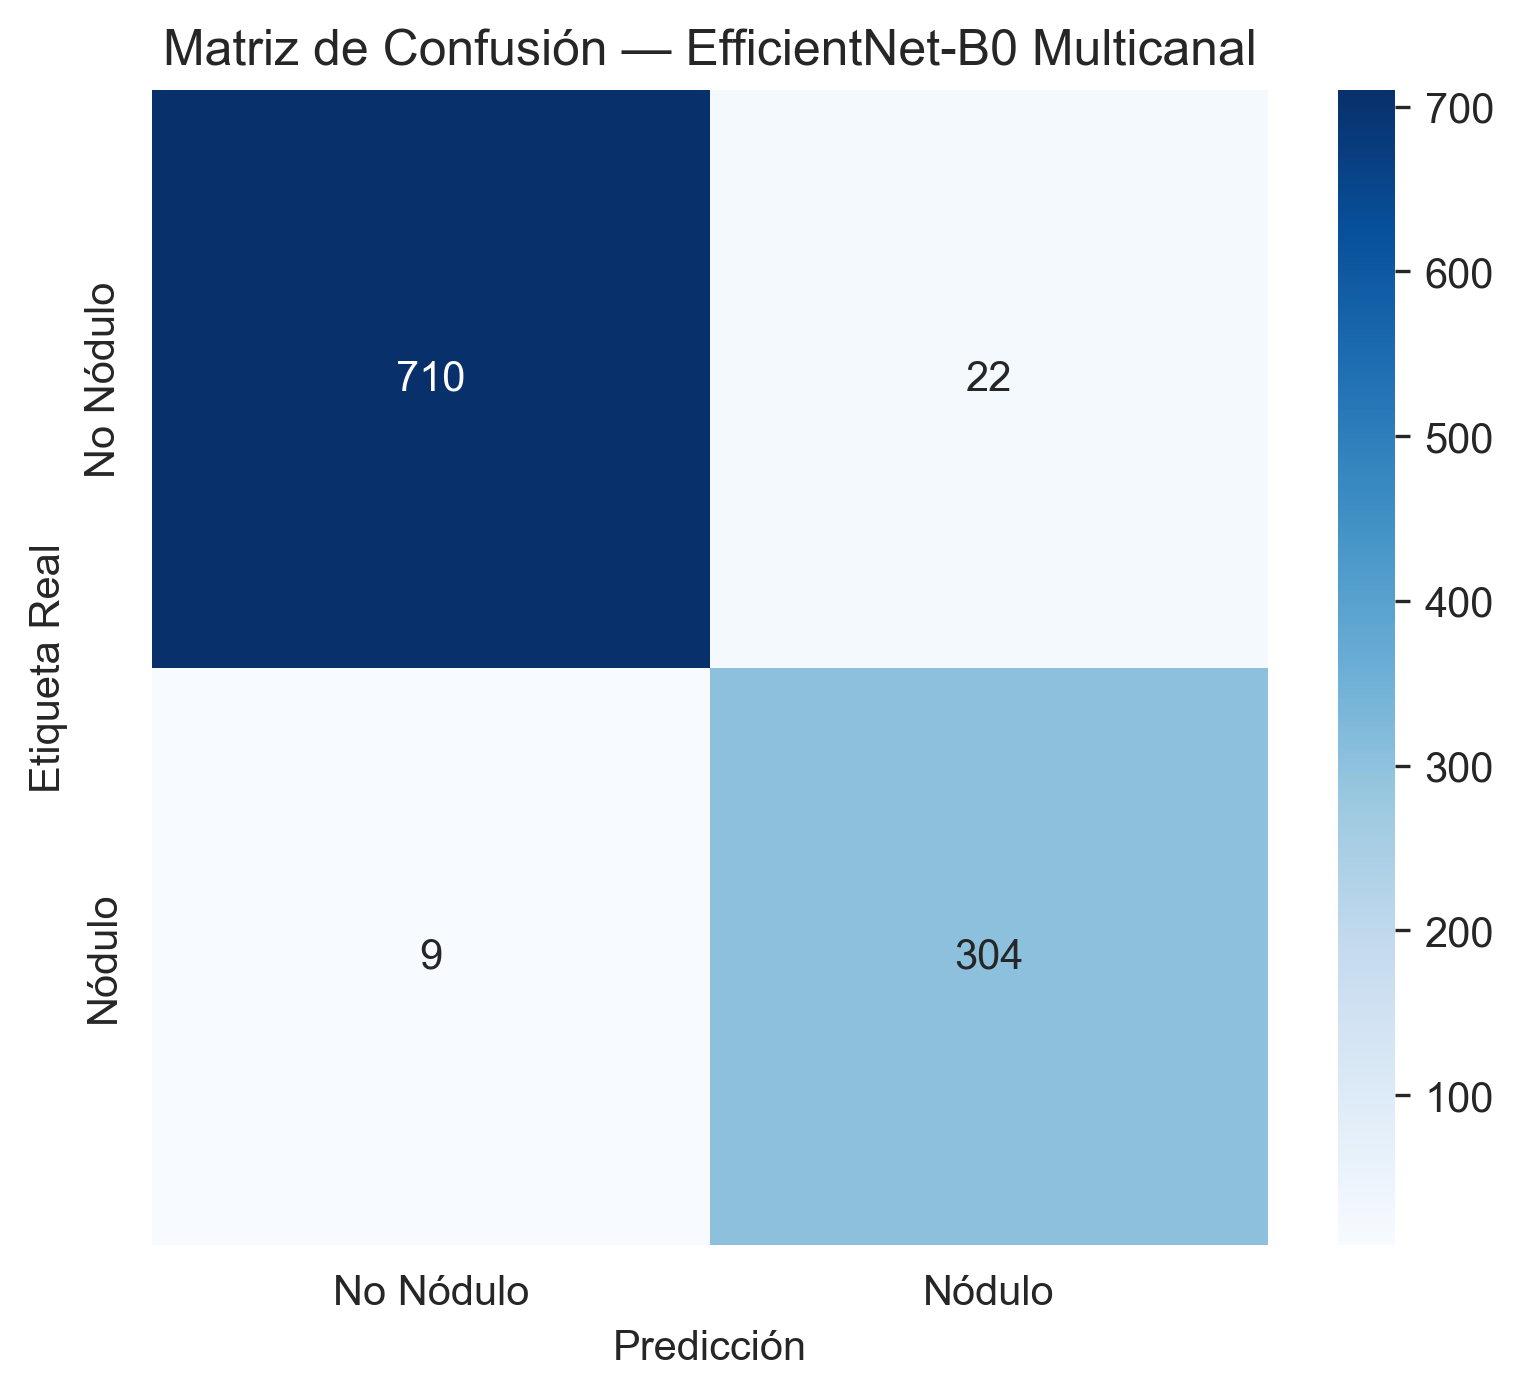
\includegraphics[width=0.60\textwidth]{images/efficientnet_b0_confusion_matrix.png}
    \caption{Matriz de confusión obtenida para el modelo EfficientNet-B0 multicanal. Se observa un excelente equilibrio entre sensibilidad y precisión, con sólo 22 falsos positivos y 9 falsos negativos sobre un total de 1045 muestras.}
    \label{fig:effb0_confusion_matrix}
\end{figure}
on:

\begin{itemize}
    \item 710 són veritables negatius (classe 0 correcta).
    \item 304 són veritables positius (classe 1 correcta).
    \item 22 són falsos positius (casos sense nòdul classificats erròniament com a nòdul).
    \item 9 són falsos negatius (nòduls no detectats).
\end{itemize}

\subsubsection{Interpretació detallada dels resultats}

Des del punt de vista clínic i tècnic, els resultats són especialment destacables:

\paragraph{Classe 0 (no nòdul).}
\begin{itemize}
    \item \textbf{Precisió} = 0.9875: el model gairebé mai etiqueta un cas com a nòdul quan en realitat no ho és.
    \item \textbf{Recall} = 0.9699: el 96.99\% dels casos sans són identificats correctament.
    \item \textbf{F1-score} = 0.9786: equilibri excel·lent entre precisió i sensibilitat.
\end{itemize}

Aquest comportament és molt valuós perquè minimitza el nombre de falsos positius i, per tant, redueix
alarmisme innecessari i sobrecàrrega de segones lectures.

\paragraph{Classe 1 (nòdul).}
\begin{itemize}
    \item \textbf{Precisió} = 0.9325: quan el model indica que hi ha nòdul, en el 93\% dels casos té raó.
    \item \textbf{Recall} = 0.9712: el model detecta aproximadament el 97\% dels nòduls reals.
    \item \textbf{F1-score} = 0.9515: combinació molt equilibrada de sensibilitat i precisió.
\end{itemize}

Els falsos negatius (9 sobre 313) representen un percentatge molt reduït i situen el model en un escenari
de sensibilitat molt elevat, especialment rellevant en tasques de cribratge on l’objectiu principal és
no deixar escapar lesions potencialment rellevants.

\subsubsection{Discussió i conclusions}

Els resultats obtinguts amb aquest model situen EfficientNet-B0 multicanal amb dataset balancejat com la
millor estratègia de classificació dins de tots els experiments realitzats fins al moment. En particular:

\begin{itemize}
    \item Millora de forma clara tant l’\textit{accuracy} global (\(0.9703\)) com el F1 de la classe positiva
          (\(\approx 0.95\)) respecte de les arquitectures provades en fases prèvies.
    \item La combinació de \textbf{multicanal} (original + CLAHE + Canny) permet al model accedir a informació
          complementària sobre intensitat, contrast local i estructura geomètrica del nòdul, d’una manera molt
          alineada amb la lectura visual que faria un radiòleg.
    \item El \textbf{dataset balancejat} evita biaixos forts cap a la classe negativa i obliga el model a aprendre
          patrons discriminatius reals de la classe positiva.
    \item L’ús d’\textbf{augmentació mèdica} moderada incrementa la robustesa del model davant petites variacions
          de posició, soroll i contrast.
\end{itemize}

En conjunt, aquest experiment demostra que, amb un disseny adequat del preprocessament i una estratègia
curada de construcció del dataset, és possible assolir rendiments molt competitius en la detecció de
nòduls pulmonars a partir de radiografies de tòrax, situant aquest model com a referència principal per a
les fases posteriors del treball (estudi d’ablació i anàlisi comparativa més detallada).

\subsubsection{Model definitiu: extensió del model multicanal de 3 a 4 canals}

En l'experiment previ es va emprar un model multicanal basat en tres representacions derivades de cada radiografia de tòrax (CXR): la imatge original normalitzada, una versió amb realç de contrast mitjançant CLAHE i un mapa de contorns obtingut amb el detector de Canny. Aquest enfocament ja va permetre millorar de manera notable el rendiment respecte a utilitzar únicament la imatge en escala de grisos, especialment pel que fa a la sensibilitat en la detecció de nòduls petits.

Tanmateix, després d'analitzar els resultats i revisar com treballen els radiòlegs en la pràctica clínica, es va identificar l’oportunitat d’enriquir encara més aquesta representació multicanal. En la lectura real de les imatges, la detecció de nòduls no es basa només en el contrast i el contorn, sinó també en la inspecció de \textit{textures fines}, microdetalls i canvis subtils en l’estructura del parènquima pulmonar.

Per aquest motiu, es va decidir incorporar un \textbf{quart canal} basat en la tècnica d’\textit{Unsharp Mask}, que realça les components d’alta freqüència de la imatge. Aquesta operació permet destacar irregularitats suaus, vores fines i patrons microestructurals que poden ser característics de lesions nodulars i que sovint són rellevants en la pràctica radiològica.

Així, el model passa a treballar amb quatre canals d’entrada per a cada CXR:

\begin{itemize}
    \item \textbf{Canal 1}: imatge original normalitzada (informació d’intensitat global).
    \item \textbf{Canal 2}: CLAHE (realç de contrast local i estructures de baix relleu).
    \item \textbf{Canal 3}: contorns de Canny (informació geomètrica i vores ben definides).
    \item \textbf{Canal 4}: Unsharp Mask (textures fines i contorns suaus realçats).
\end{itemize}

Aquest conjunt de canals aproxima de manera més fidel el procés cognitiu que segueixen els radiòlegs quan interpreten una radiografia de tòrax, combinant informació de contrast, estructura i textura per decidir si hi ha un nòdul o no. L’objectiu d’aquesta extensió és repetir l’experiment anterior amb la nova representació de quatre canals i avaluar si aquesta informació addicional permet construir un \textit{pipeline} més complet i robust, alineat amb el procés diagnòstic humà.

La Figura~\ref{fig:rx_4_capas} mostra un exemple d’una radiografia amb les quatre representacions utilitzades pel model.

\begin{figure}[H]
    \centering
    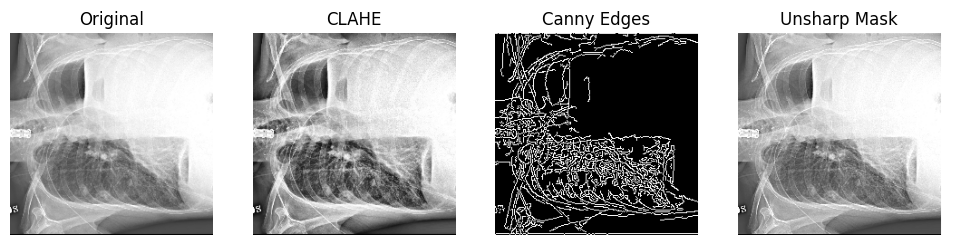
\includegraphics[width=0.95\textwidth]{images/rx_4_capas.png}
    \caption{Visualització dels quatre canals emprats en el model multicanal: 
    (1) imatge original normalitzada, 
    (2) CLAHE per al realç de contrast, 
    (3) detecció de contorns mitjançant Canny i 
    (4) realç de detalls amb Unsharp Mask. 
    Aquesta representació multicanal imita el procés interpretatiu del radiòleg en analitzar textura, contrast i geometria del nòdul.}
    \label{fig:rx_4_capas}
\end{figure}

Pel que fa al \textit{data augmentation}, s’ha adaptat de manera mínima per operar sobre tensors de quatre canals, mantenint únicament transformacions considerades clínicament segures, com ara el gir horitzontal, la rotació suau i l’addició controlada de renou gaussià. La resta del \textit{pipeline} (dataset balancejat, arquitectura EfficientNet-B0, estratègia d’entrenament i esquema d’avaluació) s’ha mantingut idèntica a l’experiment anterior, de manera que l’efecte del quart canal es pugui analitzar de forma aïllada.

El model definitiu es basa, per tant, en \textbf{EfficientNet-B0 multicanal amb 4 canals} entrenat sobre un \textit{dataset} balancejat derivat de NODE21, amb una partició aproximada del 80\,\% per a entrenament i del 20\,\% per a test. El conjunt de test final conté \textbf{1500 imatges}, amb una distribució pràcticament equilibrada entre classes: 751 radiografies sense nòdul (classe~0) i 749 amb nòdul (classe~1). A partir d’aquesta configuració es presenten, en les seccions següents, els resultats quantitatius detallats i l’anàlisi de rendiment del model.


\subsubsection{Resultats quantitatius}

El \textit{classification report} obtingut sobre el conjunt de test és el següent:

\begin{table}[H]
    \centering
    \caption{Resultats del model EfficientNet-B0 multicanal (4 canals) sobre el conjunt de test.}
    \label{tab:effb0_4c_report}
    \begin{tabular}{lcccc}
        \toprule
        \textbf{Classe} & \textbf{Precisió} & \textbf{Recall} & \textbf{F1-score} & \textbf{Suport} \\
        \midrule
        0 (no nòdul) & 0.9892 & 0.9720 & 0.9805 & 751 \\
        1 (nòdul)    & 0.9724 & 0.9893 & 0.9808 & 749 \\
        \midrule
        \textbf{Exactitud global} & \multicolumn{4}{c}{0.9807} \\
        \textbf{Mitjana macro}    & 0.9808 & 0.9807 & 0.9807 & 1500 \\
        \textbf{Mitjana ponderada}& 0.9808 & 0.9807 & 0.9807 & 1500 \\
        \bottomrule
    \end{tabular}
\end{table}

Aquests resultats mostren diversos aspectes destacables:

\begin{itemize}
    \item L'\textbf{exactitud global} (\emph{accuracy}) és del 98.07\,\%, valor molt elevat per a una tasca de classificació de nòduls en radiografies frontals de tòrax.
    \item La \textbf{classe 0} (sense nòdul) presenta una precisió de 0.9892 i un recall de 0.9720, amb un F1-score de 0.9805. Això indica que el model gairebé no genera falsos positius i que identifica correctament la majoria de radiografies normals.
    \item La \textbf{classe 1} (amb nòdul) assoleix una precisió de 0.9724 i un recall de 0.9893, amb un F1-score de 0.9808. En termes pràctics, això significa que el model detecta prop del 99\,\% dels nòduls presents al conjunt de test, amb un nombre molt reduït de falsos positius.
    \item La \textbf{mitjana macro} i la \textbf{mitjana ponderada} són pràcticament idèntiques (al voltant de 0.98 en totes les mètriques), la qual cosa suggereix que el comportament del model és molt equilibrat entre classes, sense biaixar-se excessivament cap als casos negatius.
\end{itemize}

\subsubsection{Matriu de confusió}

La matriu de confusió associada a aquests resultats es mostra a la Taula~\ref{tab:effb0_4c_confusion}. Els valors exactes són:

\begin{figure}[H]
    \centering
    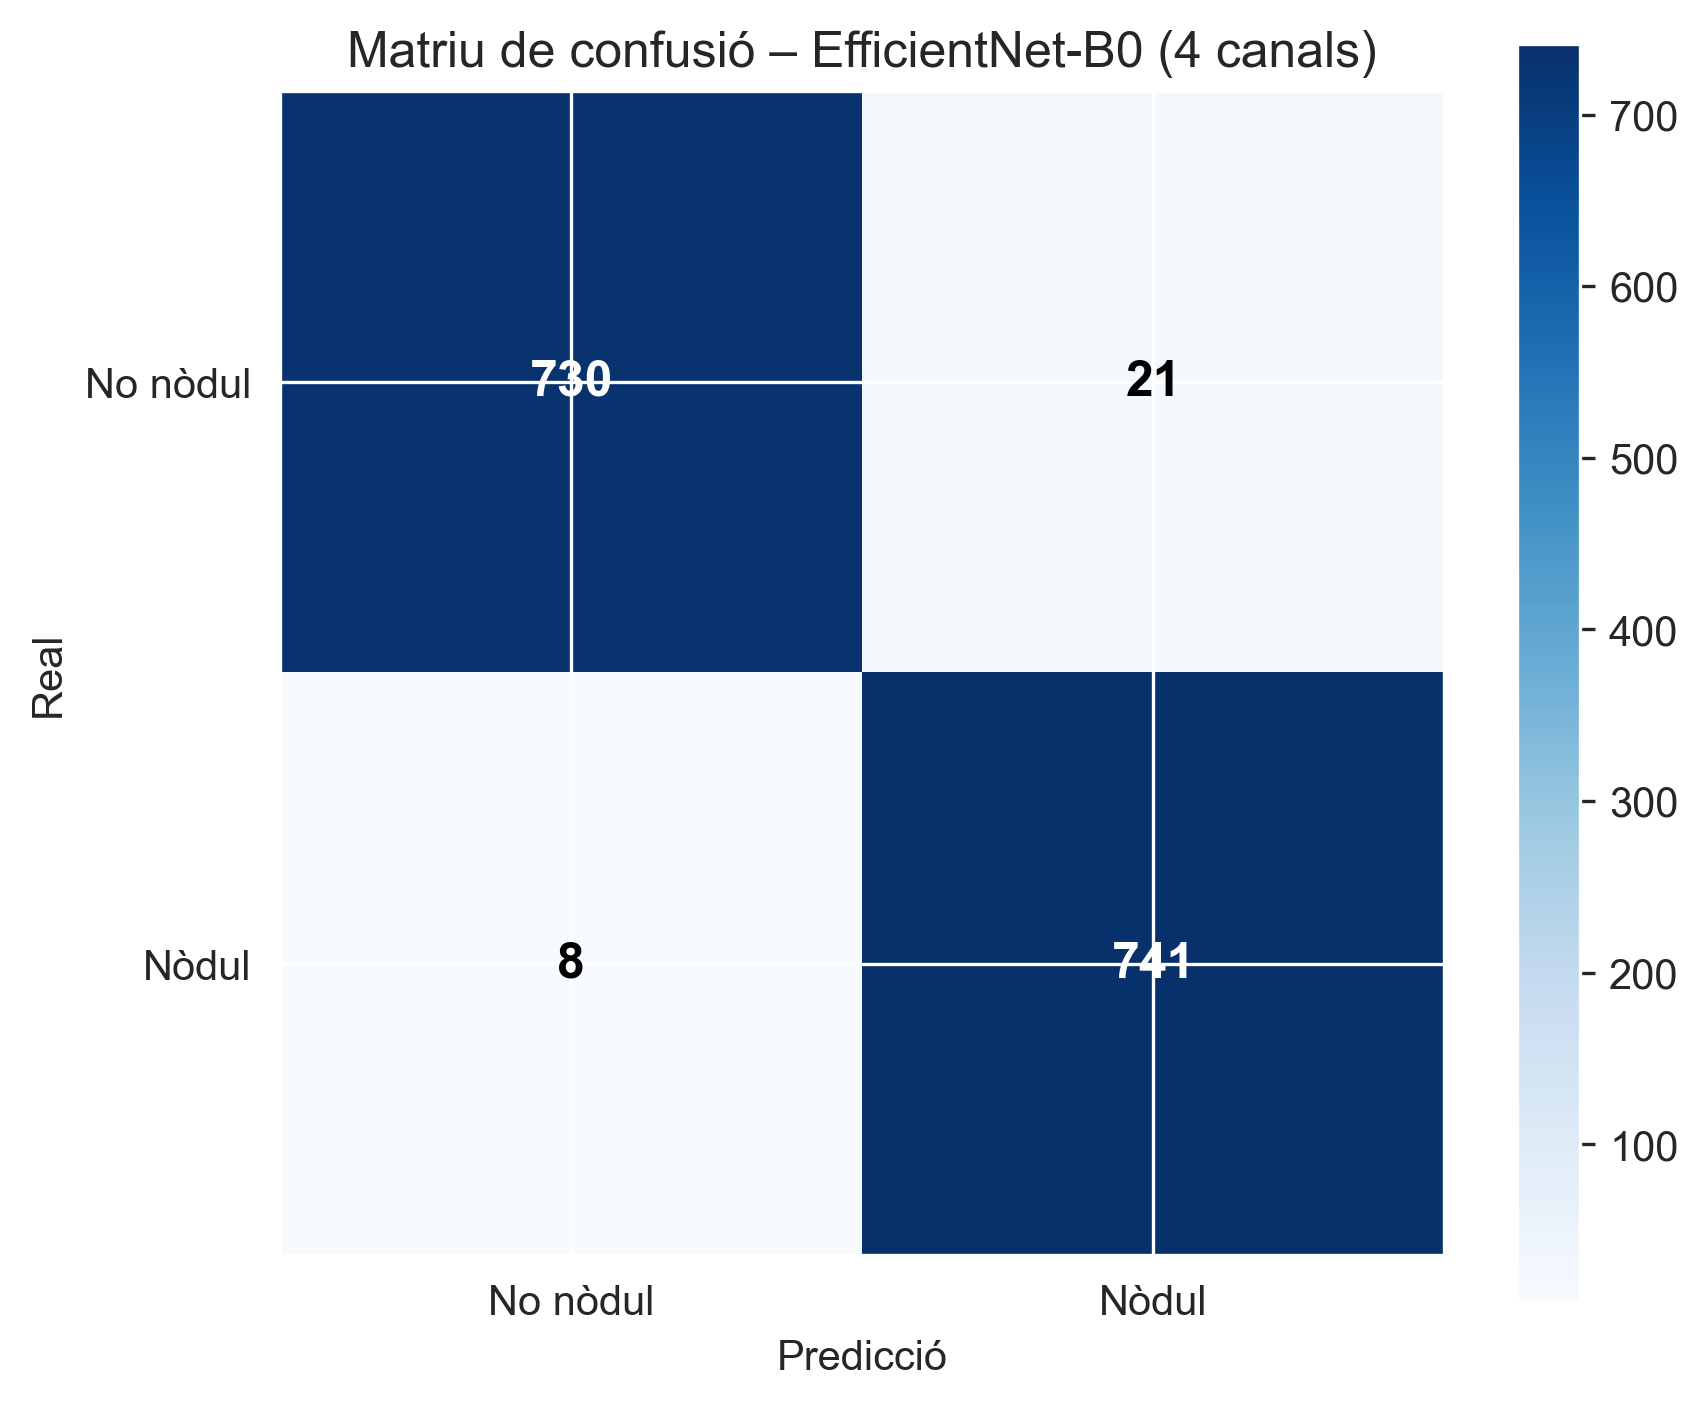
\includegraphics[width=0.6\textwidth]{images/confusion_matrix_efficientnetb0_4canales.png}
    \caption{Matriu de confusió del model \textit{EfficientNet-B0} multicanal (4 canals) sobre el conjunt de test. 
    Els tons de blau indiquen la concentració de prediccions correctes i errònies, destacant l’elevada sensibilitat i precisió del model tant per a la classe negativa com per a la positiva.}
    \label{fig:effb0_4c_confusion}
\end{figure}

On:

\begin{itemize}
    \item 730 són \textbf{veritables negatius} (radiografies sense nòdul classificades correctament com a classe 0).
    \item 21 són \textbf{falsos positius} (radiografies sense nòdul que el model etiqueta erròniament com a nòdul).
    \item 8 són \textbf{falsos negatius} (radiografies amb nòdul que el model no detecta).
    \item 741 són \textbf{veritables positius} (radiografies amb nòdul detectades correctament).
\end{itemize}




Des d'un punt de vista clínic, els indicadors més rellevants són:

\begin{itemize}
    \item Els \textbf{falsos negatius} (8 casos) representen aproximadament un 1.1\,\% dels 749 nòduls reals. Aquest valor és molt baix i indica una sensibilitat (recall) molt alta per a la classe positiva.
    \item Els \textbf{falsos positius} (21 casos) corresponen aproximadament a un 2.8\,\% de les 751 radiografies sense nòdul. Això implica que el sistema genera poques alarmes innecessàries, mantenint una alta precisió en la detecció de nòduls.
\end{itemize}

En conjunt, la matriu de confusió confirma que el model és capaç de mantenir, alhora, una \textbf{sensibilitat molt elevada} per als nòduls i una \textbf{taxa de falsos positius moderada}, condicions desitjables en un sistema de suport a la decisió clínica.

\subsubsection{Evolució de la pèrdua i de l'exactitud durant l'entrenament}

La Figura~\ref{fig:effb0_4c_training} mostra l'evolució de la pèrdua (\emph{loss}) i de l'exactitud (\emph{accuracy}) durant les 20 èpoques d'entrenament del model EfficientNet-B0 de 4 canals. Per cada època es registra la pèrdua mitjana sobre el conjunt d'entrenament i l'exactitud global assolida.
\begin{figure}[H]
    \centering
    \begin{subfigure}[t]{0.48\textwidth}
        \centering
        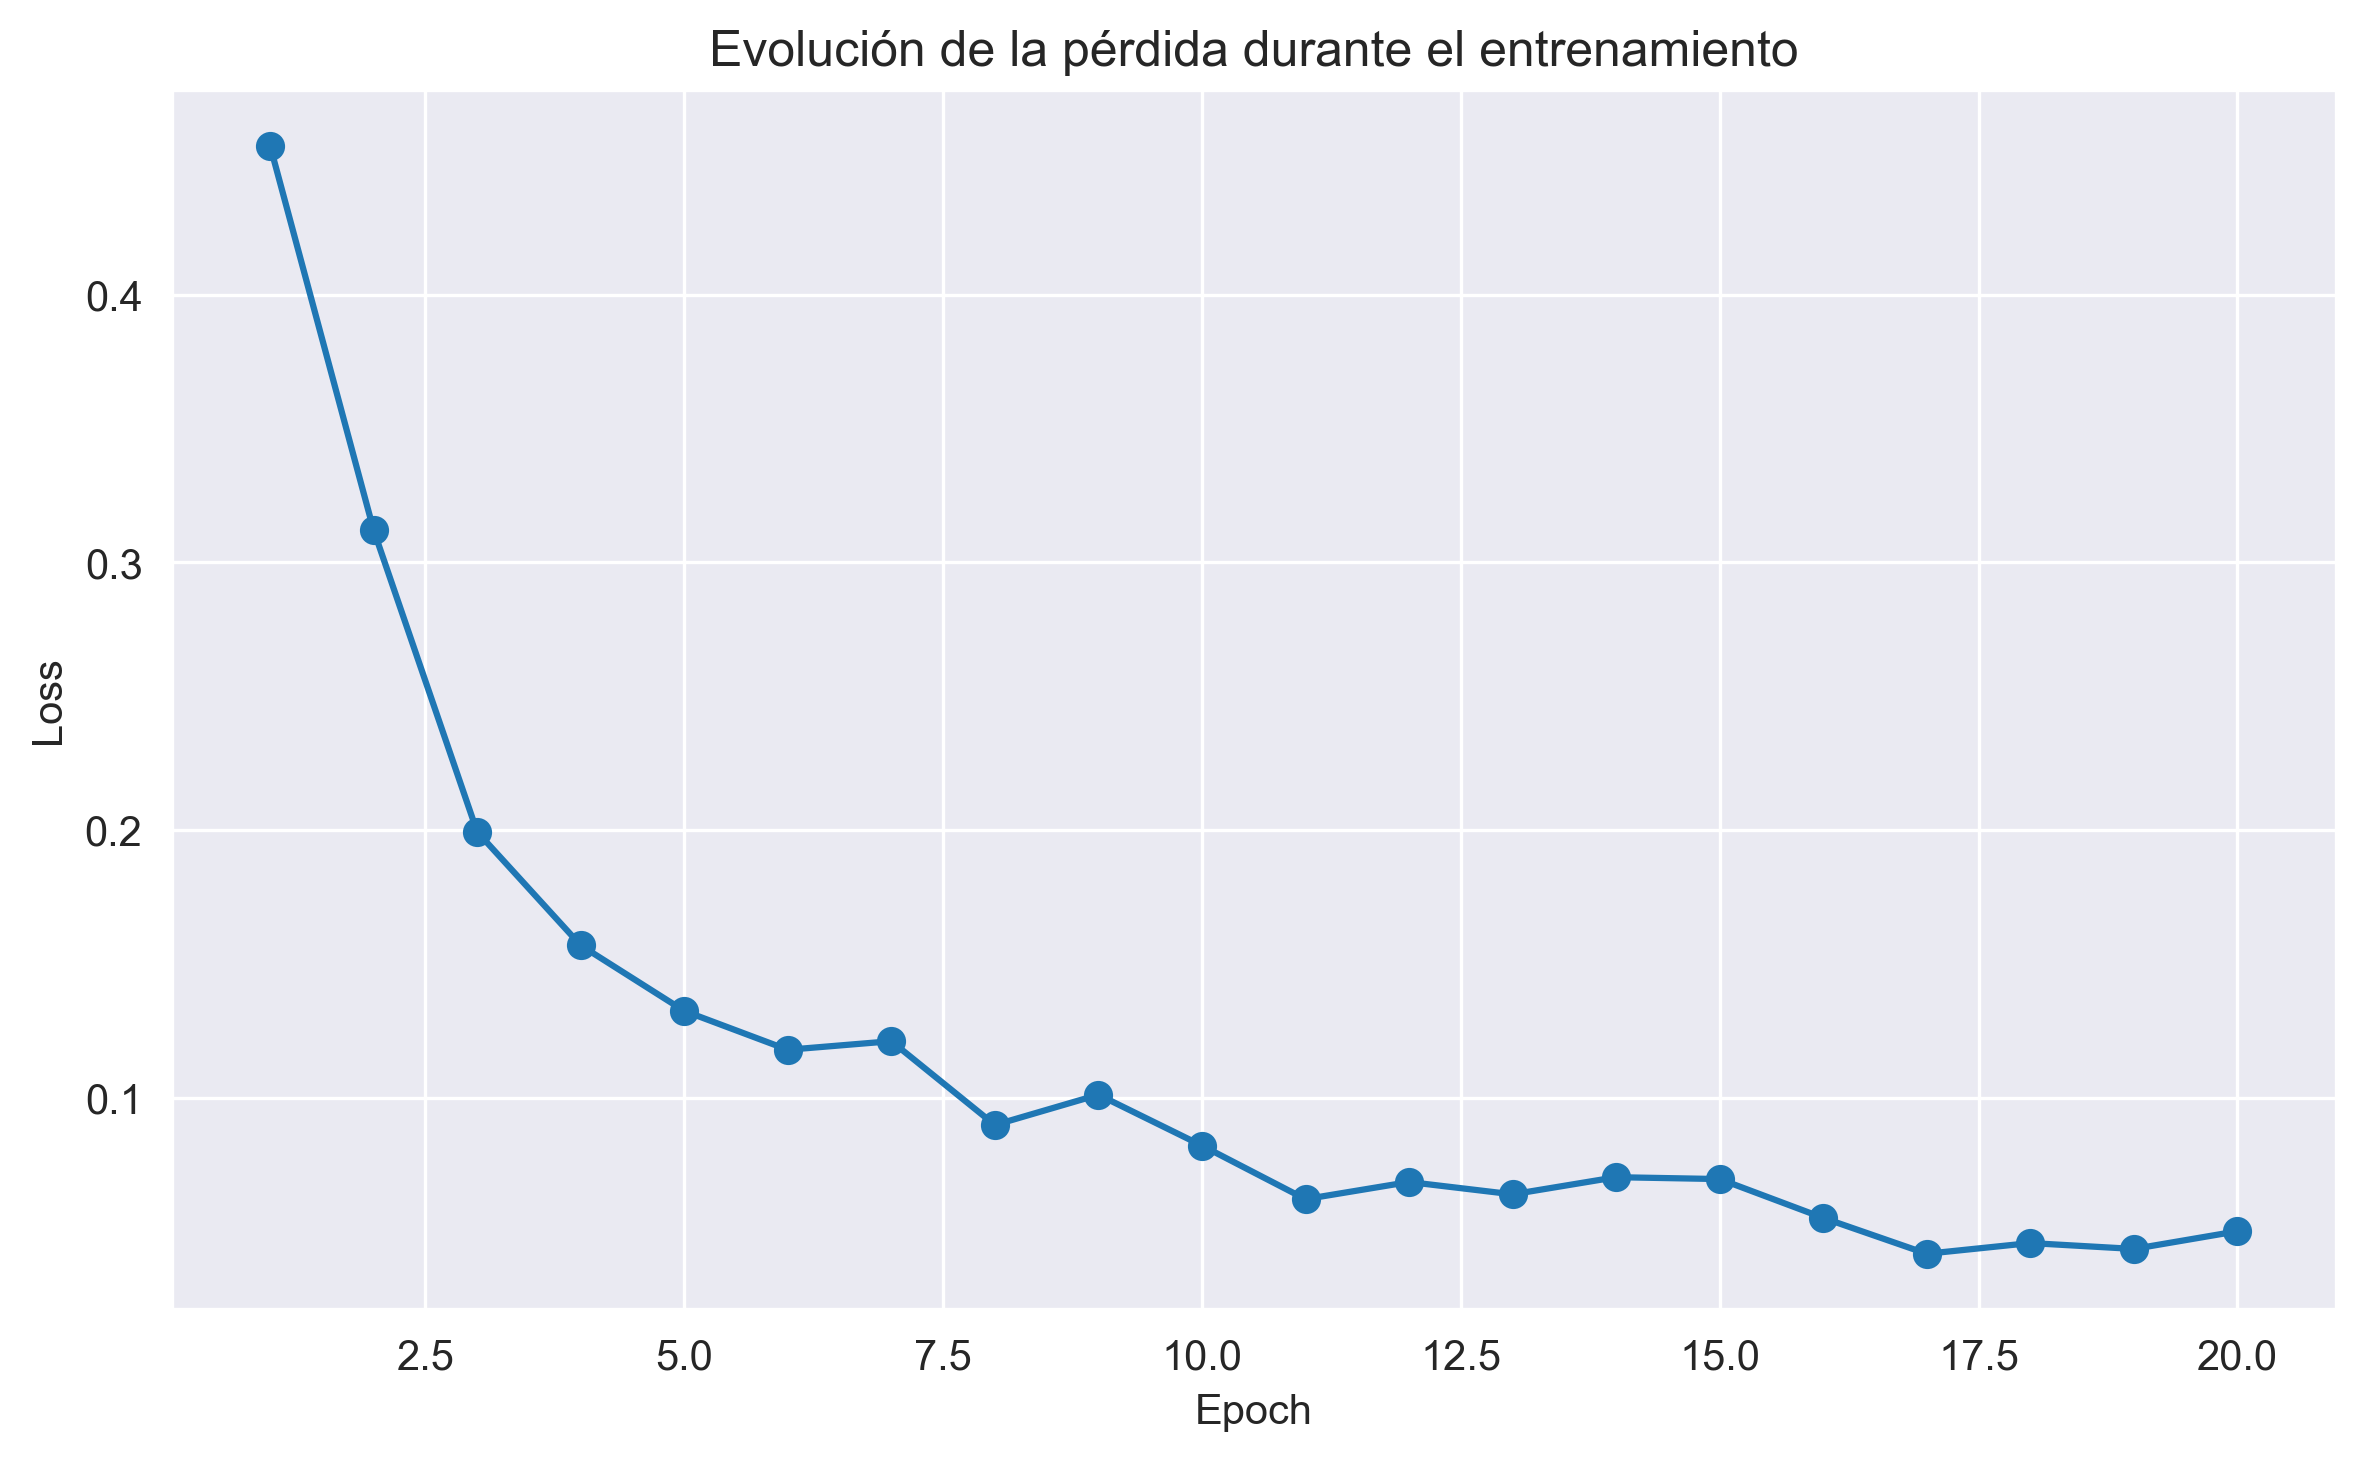
\includegraphics[width=\textwidth]{images/loss_final_efficientnetb0_4canales.png}
        \caption{Evolució de la pèrdua (\emph{loss}) durant l'entrenament.}
        \label{fig:effb0_4c_loss}
    \end{subfigure}
    \hfill
    \begin{subfigure}[t]{0.48\textwidth}
        \centering
        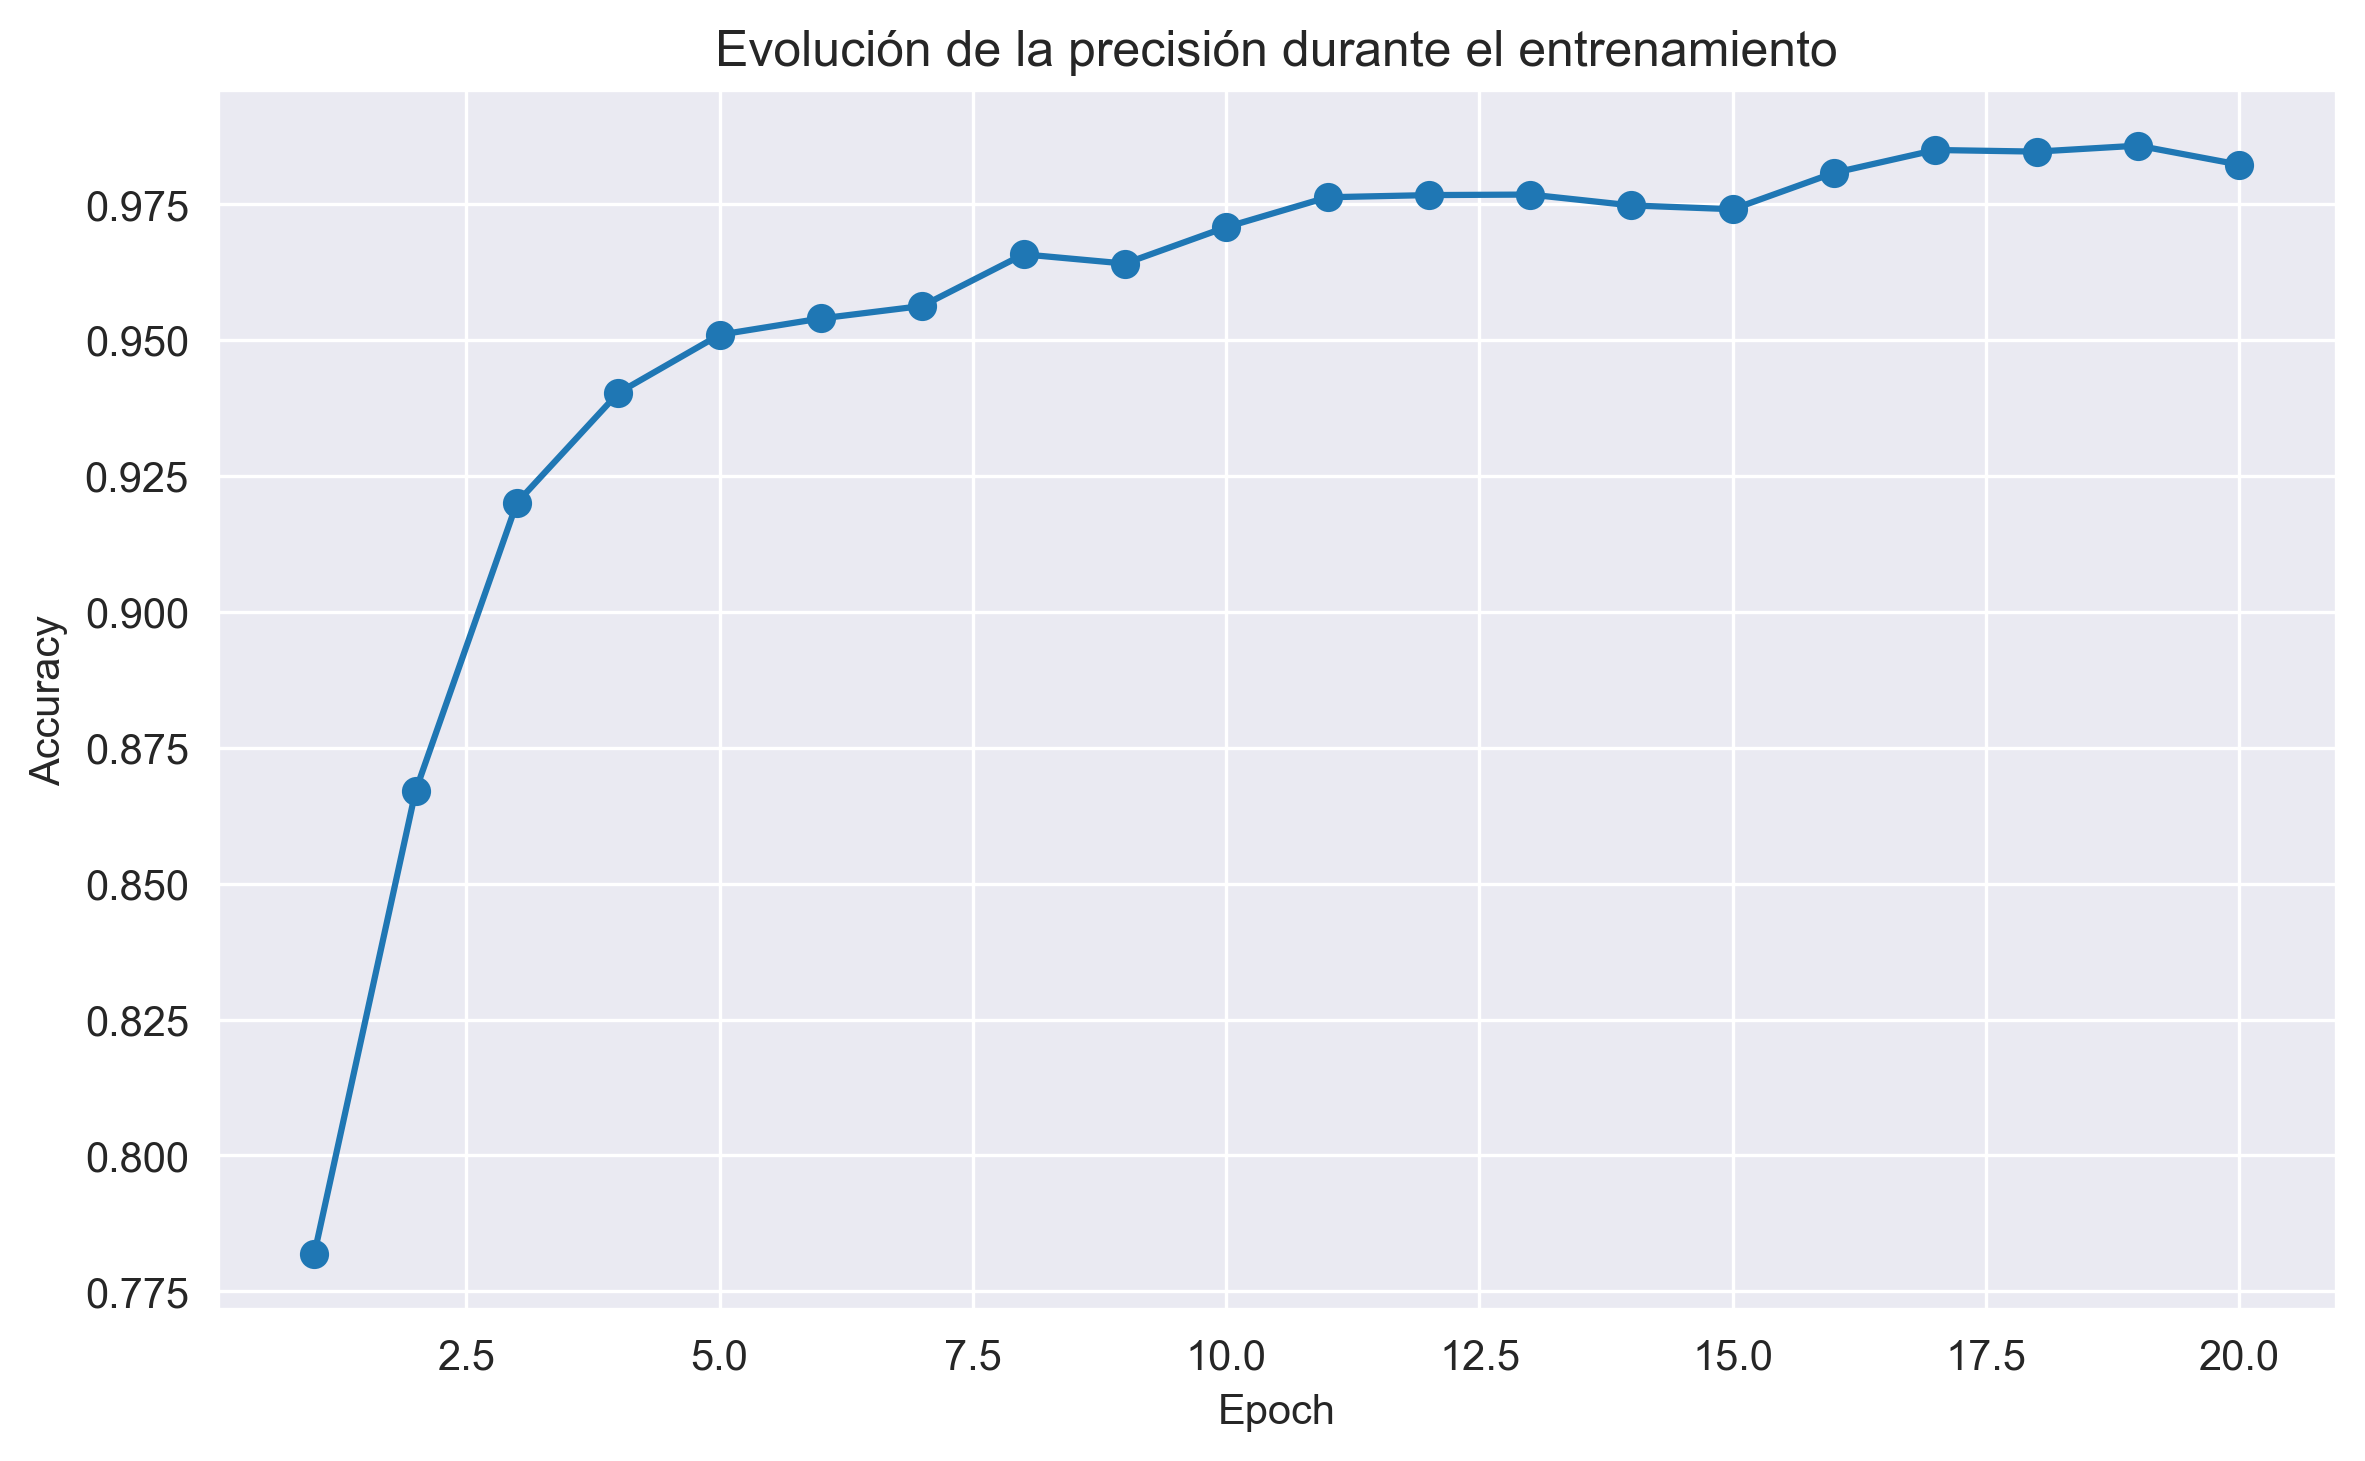
\includegraphics[width=\textwidth]{images/accuracy_final_efficientnetb0_4canales.png}
        \caption{Evolució de l'exactitud (\emph{accuracy}) durant l'entrenament.}
        \label{fig:effb0_4c_accuracy}
    \end{subfigure}

    \caption{Evolució de la pèrdua (\emph{loss}) i de l'exactitud (\emph{accuracy}) durant les 20 èpoques d'entrenament del model EfficientNet-B0 multicanal amb quatre canals d'entrada.}
    \label{fig:effb0_4c_training}
\end{figure}


Els valors numèrics mostren que:

\begin{itemize}
    \item La \textbf{pèrdua d'entrenament} decreix de forma progressiva des d'aproximadament 0.45 en la primera època fins a valors propers a 0.05 en les darreres èpoques.
    \item L'\textbf{exactitud d'entrenament} creix des d'un 78.19\,\% en la primera època fins a un 98.23\,\% en la vintena època. Ja a partir de l'època 10 se superen valors del 97\,\%, indicant que el model convergeix cap a una solució de molt alt rendiment.
    \item No s'observa cap augment significatiu de la pèrdua ni caiguda de l'exactitud en les últimes èpoques, la qual cosa suggereix que no hi ha un sobreajust (\emph{overfitting}) sever sobre el conjunt d'entrenament.
\end{itemize}


Finalment, si es comparen aquests resultats amb els models provats en fases prèvies (CNN simple, ResNet-18, DenseNet-121, EfficientNet-B0 amb 1 canal, EfficientNet-B3, DenseNet-169 multicanal, etc.), es constata que l'arquitectura \textbf{EfficientNet-B0 multicanal amb 4 canals} i \textbf{dataset balancejat} és la que ofereix el millor compromís global entre sensibilitat, especificitat i estabilitat d'entrenament, constituint el \emph{pipeline} definitiu dins d'aquest estudi.


\begin{figure}[H]
    \centering
    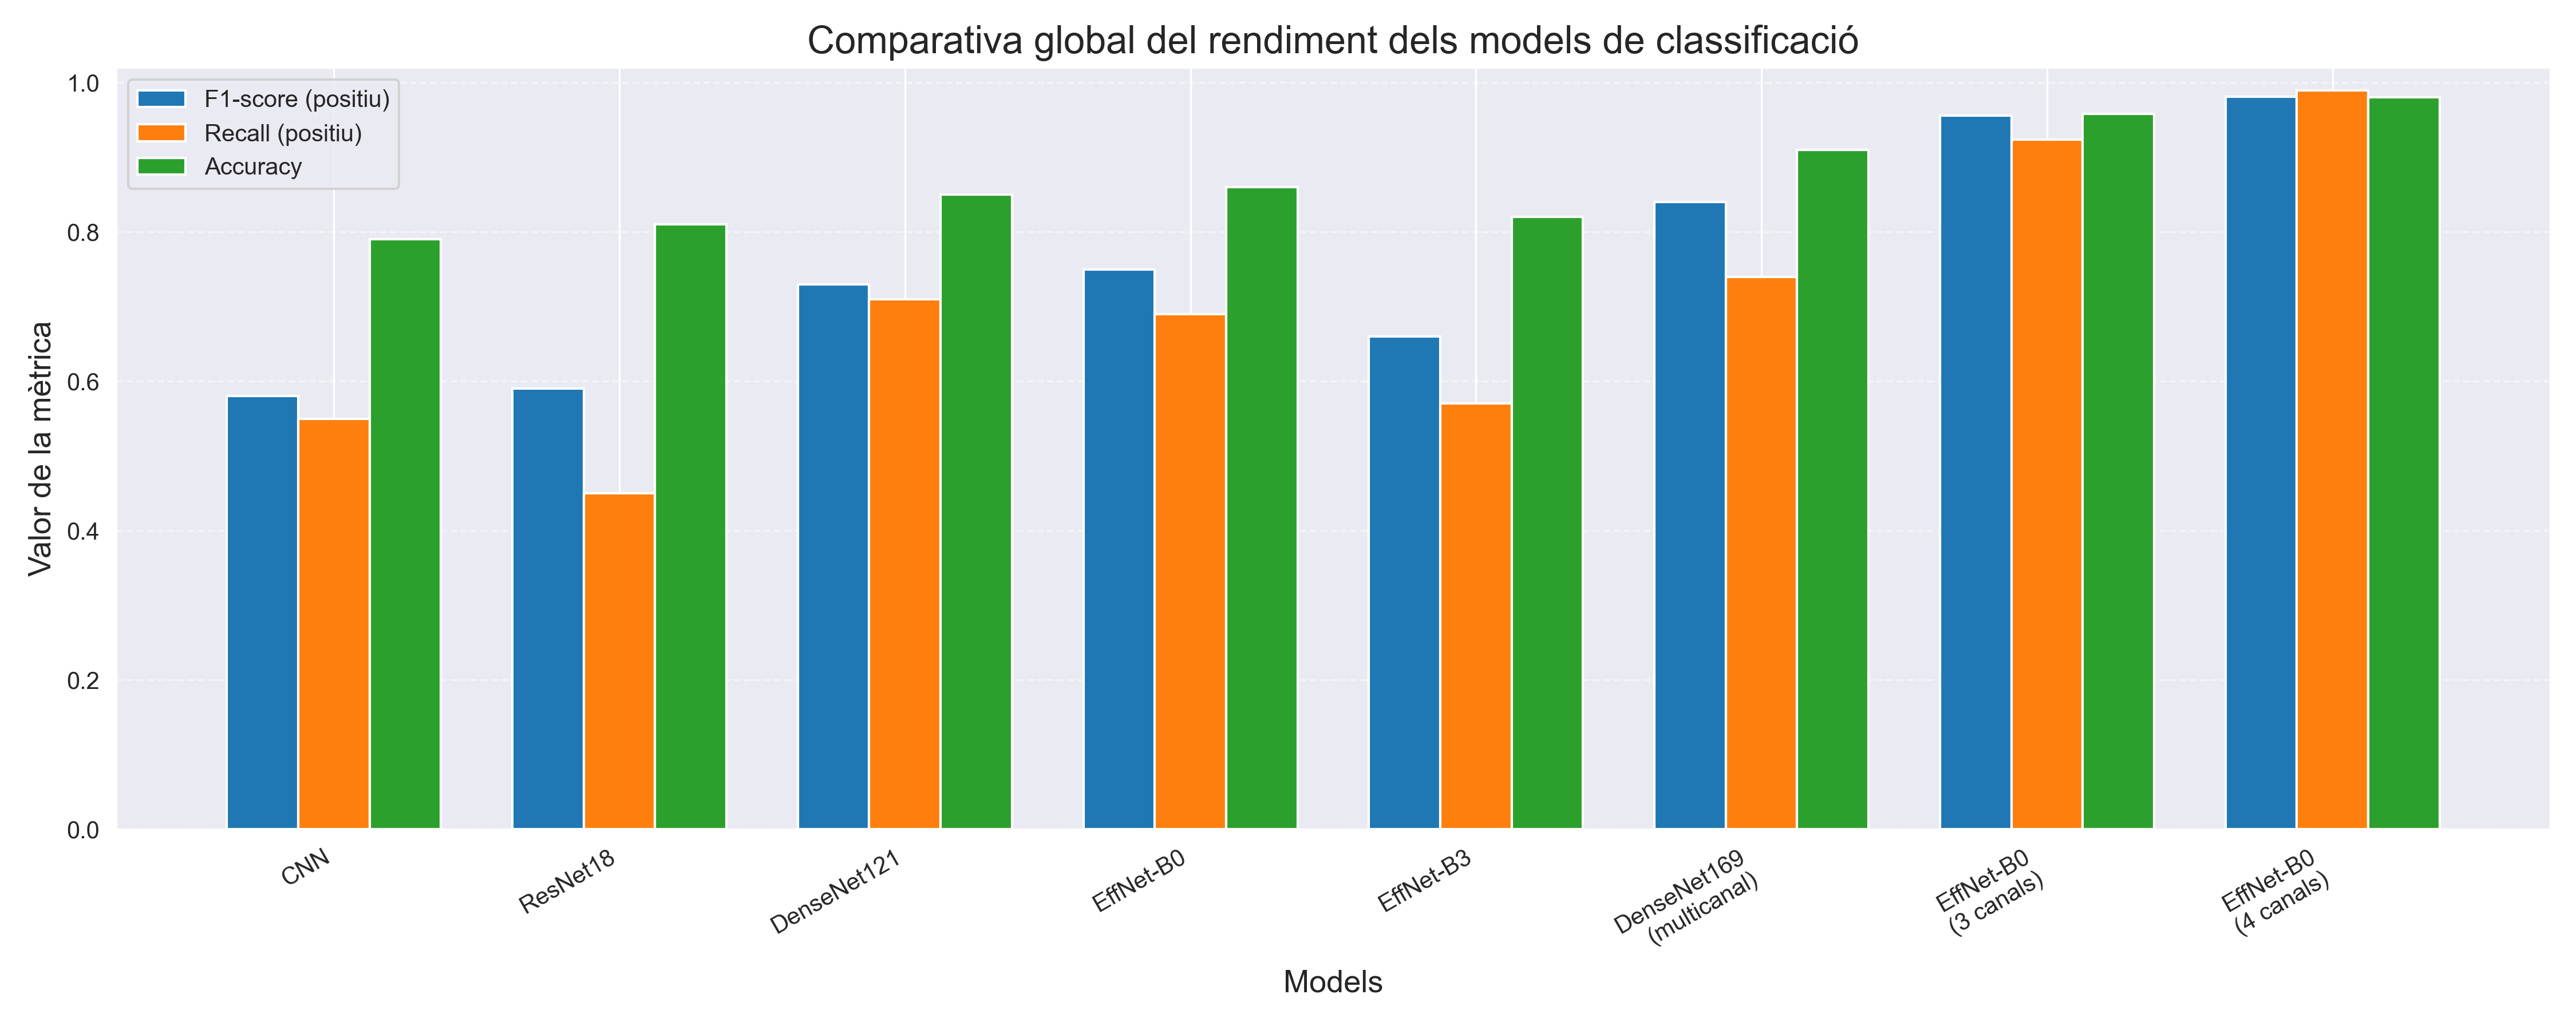
\includegraphics[width=0.98\textwidth]{images/comparativa_models_classificacio.png}
    \caption{
    Comparativa global del rendiment dels diferents models de classificació avaluats al llarg de l’estudi.
    Es mostren les mètriques d’\emph{accuracy}, \emph{recall} de la classe positiva (sensibilitat clínica)
    i \emph{F1-score} de la classe positiva per als models CNN simple, ResNet-18, DenseNet-121,
    EfficientNet-B0 i B3 amb un sol canal, DenseNet-169 multicanal, i les versions multicanal
    d’EfficientNet-B0 amb tres i quatre canals.
    S’observa una millora progressiva del rendiment amb l’ús de tècniques de \emph{transfer learning},
    representacions multicanal i dataset balancejat, destacant clarament el model
    EfficientNet-B0 multicanal amb quatre canals com el que ofereix el millor compromís global
    entre sensibilitat, precisió i estabilitat d’entrenament.
    }
    \label{fig:comparativa_models}
\end{figure}



\section{Estudi d’Ablació del Pipeline Multicanal}

Un cop identificada EfficientNet-B0 com l’arquitectura amb el millor compromís entre
rendiment i estabilitat, es va dur a terme un estudi d’ablació amb l’objectiu d’analitzar
de manera sistemàtica la contribució de cada canal d’informació afegit al pipeline
multicanal. Aquest estudi permet quantificar l’impacte real de cada tipus de
preprocessament i justificar de manera objectiva la configuració final seleccionada.

L’anàlisi es va realitzar de forma incremental, partint d’una representació monocanal
i afegint progressivament canals derivats basats en tècniques de millora de contrast,
detecció de vores i realç d’altes freqüències. En tots els experiments es van mantenir
constants el dataset balancejat, l’arquitectura EfficientNet-B0, els hiperparàmetres
d’entrenament i el procediment d’avaluació, garantint així la comparabilitat directa
dels resultats.


\subsection{Configuracions Avaluades}

Es van analitzar de manera sistemàtica les configuracions següents, amb l’objectiu
d’avaluar tant l’impacte individual de cada transformació com el seu efecte combinat
dins del pipeline multicanal:

\begin{itemize}
    \item \textbf{1 canal (Original)}: imatge original normalitzada.
    \item \textbf{1 canal (Canny)}: imatge original transformada mitjançant detecció de vores Canny.
    \item \textbf{1 canal (Unsharp)}: imatge original amb realç d’altes freqüències mitjançant Unsharp Mask.
    \item \textbf{2 canals}: imatge original + millora de contrast local mitjançant CLAHE.
    \item \textbf{3 canals (CLAHE + Canny)}: imatge original + CLAHE + detecció de vores Canny.
    \item \textbf{3 canals (CLAHE + Unsharp)}: imatge original + CLAHE + Unsharp Mask.
    \item \textbf{4 canals}: imatge original + CLAHE + Canny + Unsharp Mask.
\end{itemize}


\subsection{Resultats Quantitatius}

La Taula~\ref{tab:ablation_results} resumeix els principals resultats obtinguts al conjunt
de test per a cada configuració. A més de l’accuracy global, s’inclouen mètriques
clíniques rellevants com el \textit{recall} de la classe positiva, el nombre de falsos
negatius (FN) i de falsos positius (FP).

\begin{table}[H]
\centering
\scriptsize
\renewcommand{\arraystretch}{1.1}
\begin{tabular}{c c c c c c}
\toprule
\textbf{Can.} & \textbf{Configuració} & \textbf{Acc.} & \textbf{Rec.(1)} & \textbf{FN} & \textbf{FP} \\
\midrule
1 & Original & 0.9667 & 0.9573 & 32 & 18 \\
1 & Canny & 0.9173 & 0.8478 & 114 & 10 \\
1 & Unsharp & 0.9673 & 0.9546 & 34 & 15 \\
2 & Orig.+CLAHE & \textbf{0.9813} & \textbf{0.9933} & \textbf{5} & 23 \\
3 & Orig.+CLAHE+Canny & 0.9713 & 0.9693 & 23 & 20 \\
3 & Orig.+CLAHE+Unsharp & 0.9800 & 0.9706 & 22 & \textbf{8} \\
4 & Orig.+CLAHE+Canny+Unsharp & 0.9813 & 0.9800 & 15 & 13 \\
\bottomrule
\end{tabular}
\caption{Resultats de l’estudi d’ablació del pipeline multicanal amb EfficientNet-B0 sobre el dataset balancejat.}
\label{tab:ablation_results}
\end{table}


\subsection{Anàlisi de l’Impacte dels Canals}

Els resultats de l’estudi d’ablació mostren diferències clares en funció del tipus de
canal utilitzat i de com s’integra dins el pipeline. La configuració monocanal amb la
imatge original proporciona una base raonable, però presenta una sensibilitat limitada,
amb un nombre apreciable de falsos negatius.

L’ús exclusiu del canal Canny produeix el pitjor rendiment global. Tot i generar una
reducció dels falsos positius, aquesta configuració presenta una caiguda molt significativa
del \textit{recall} de la classe positiva (84.78\%), amb un nombre elevat de falsos
negatius. Aquest comportament confirma que la detecció de vores dures elimina informació
clínica rellevant relacionada amb canvis subtils de densitat, essencials en la detecció
de nòduls pulmonars. En aquest context, Canny força una representació massa esquemàtica
de la imatge que no reflecteix adequadament la naturalesa difusa de moltes lesions.

La configuració monocanal basada en Unsharp Mask millora lleugerament el comportament
respecte a la imatge original, especialment en termes de detall fi, però no aporta una
millora substancial de la sensibilitat. Això indica que el realç d’altes freqüències,
per si sol, no és suficient per capturar tota la variabilitat estructural dels nòduls.

La incorporació de CLAHE com a segon canal suposa el salt qualitatiu més important del
pipeline. Aquesta configuració assoleix el major \textit{recall} de la classe positiva
(99.33\%) i el menor nombre de falsos negatius, evidenciant que el realç de contrast
local és clau per detectar nòduls de baix contrast o sub-sòlids.

Quan s’afegeix Canny com a tercer canal (Original + CLAHE + Canny), el rendiment torna a
empitjorar, reforçant la idea que la informació de vores dures pot resultar perjudicial
si no es compensa amb canals que preservin la continuïtat de la intensitat.

En canvi, la combinació de tres canals basada en Original + CLAHE + Unsharp Mask mostra
un comportament molt equilibrat, amb una reducció notable dels falsos positius i una
sensibilitat elevada. Aquesta configuració posa de manifest que el realç suau d’altes
freqüències és més adequat que la detecció binària de vores en aquest domini clínic.

Finalment, la configuració de quatre canals ofereix el millor compromís global. Tot i no
maximitzar una única mètrica de forma aïllada, presenta una combinació robusta de
sensibilitat, especificitat i estabilitat, amb una reducció simultània de falsos negatius
i falsos positius. A més, aquesta configuració mostra una menor variabilitat entre
execucions, fet que indica una major estabilitat d’entrenament.


\subsection{Interpretació Clínica i Estabilitat}

Des d’un punt de vista clínic, la minimització dels falsos negatius és un requisit
prioritari, atès que la no detecció d un nòdul pot tenir conseqüències greus en el
seguiment del pacient. Tanmateix, un excés de falsos positius també resulta problemàtic,
ja que incrementa el nombre d exploracions complementàries, genera alarmes innecessàries
i augmenta la càrrega assistencial.

En aquest equilibri entre sensibilitat i especificitat, la configuració multicanal de
quatre canals destaca per presentar un comportament més estable i consistent. Aquesta
configuració aconsegueix reduir simultàniament el nombre de falsos negatius i de falsos
positius, alhora que mostra una menor variabilitat entre execucions successives, fet que
indica una millor generalització del model.

Aquest comportament és coherent amb la pràctica radiològica real, en la qual el diagnòstic
no es fonamenta en una única transformació de la imatge, sinó en la integració visual de
diversos estímuls: contrast local, patrons de textura i realç suau del detall fi. El
pipeline multicanal de quatre canals reprodueix de manera més fidel aquest procés
perceptiu humà, permetent al model captar tant variacions globals de densitat com detalls
locals subtils sense introduir artefactes abruptes.

\subsection{Conclusió de l’Estudi d’Ablació}

L’estudi d’ablació realitzat demostra que no totes les transformacions derivades aporten
millores directes al rendiment del model i que l’impacte de cada canal depèn de la seva
integració amb la resta del pipeline. En particular, CLAHE emergeix com el component
fonamental per millorar la sensibilitat del sistema, especialment en la detecció de
nòduls de baix contrast, mentre que Unsharp Mask contribueix a reforçar la percepció del
detall fi i a millorar l’especificitat i l’estabilitat global del model.

Per contra, l’ús de canals basats exclusivament en detecció de vores dures, com Canny,
mostra limitacions importants quan s’utilitza de forma aïllada o sense mecanismes
compensatoris, ja que tendeix a eliminar informació clínica rellevant i incrementa el
nombre de falsos negatius.

Cal destacar que la configuració de \textbf{dos canals (imatge original + CLAHE)}
constitueix una alternativa plenament vàlida en escenaris clínics on la prioritat
absoluta és la minimització de falsos negatius. Aquesta configuració presenta el major
recall per a la classe positiva i el menor nombre de FN, fet que la fa especialment
adequada com a sistema de triatge o detecció precoç.

Tanmateix, la combinació final de \textbf{quatre canals} proporciona el millor compromís
global entre sensibilitat, especificitat, robustesa i estabilitat entre execucions
successives. En conseqüència, el pipeline multicanal de \textbf{quatre canals},
conjuntament amb \textbf{EfficientNet-B0} i el \textbf{dataset balancejat}, es selecciona
com la configuració definitiva com a resultat de l'estudi de classificació.


\subsection{Anàlisi d’Explicabilitat amb Integrated Gradients}

Per analitzar com el model utilitza la informació proporcionada pels diferents canals del
pipeline multicanal, s’ha aplicat la tècnica d’\textbf{Integrated Gradients} mitjançant la
llibreria Captum. Aquesta metodologia permet estimar la contribució de cada píxel de la
imatge d’entrada a la predicció final, proporcionant una explicació basada en gradients
integrats respecte a una línia base.

La Figura~\ref{fig:ig_multicanal} mostra, per a un mateix cas classificat com a
\emph{nòdul} amb elevada confiança, els mapes d’atribució associats a cadascun dels quatre
canals del pipeline: imatge original, CLAHE, Canny i Unsharp Mask.

\begin{figure}[H]
    \centering
    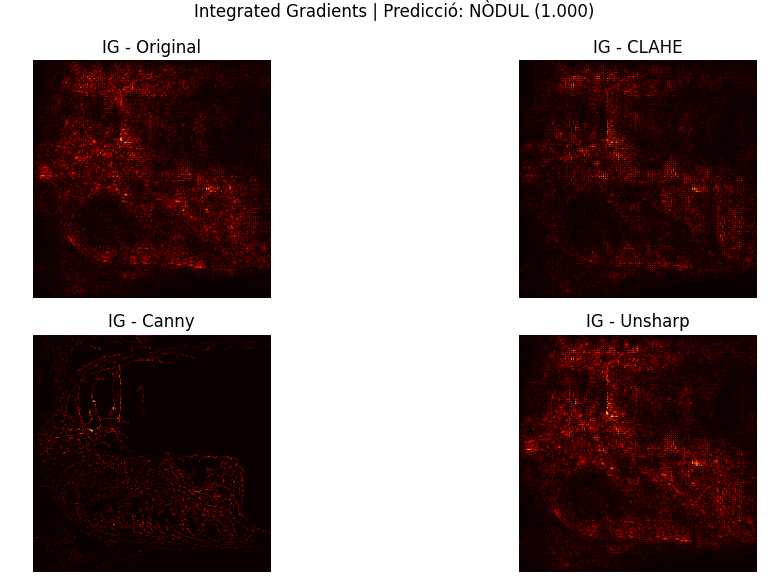
\includegraphics[width=0.9\textwidth]{images/ig_multicanal_example2.png}
    \caption{Mapes d’atribució obtinguts amb Integrated Gradients per als quatre canals del
    pipeline multicanal: original, CLAHE, Canny i Unsharp Mask.}
    \label{fig:ig_multicanal}
\end{figure}

Des d’un punt de vista qualitatiu, s’observa que els canals \textbf{Original} i
\textbf{CLAHE} presenten activacions distribuïdes principalment sobre regions pulmonars
rellevants, indicant que el model basa una part important de la seva decisió en patrons
de densitat i textura suaus. El canal \textbf{Unsharp Mask} mostra activacions més
focalitzades associades al detall fi, actuant com un reforç complementari que millora la
delimitació de zones sospitoses.

Per contra, el canal \textbf{Canny} presenta activacions disperses i fortament associades
a vores anatòmiques d’alt contrast, com costelles i estructures externes, amb una
contribució limitada a les regions clínicament rellevants. Aquest comportament és
coherent amb el rendiment inferior observat en les configuracions basades en detecció de
vores dures.

A més de l’anàlisi visual, s’ha realitzat una quantificació global de la importància de
cada canal mitjançant la suma absoluta de les atribucions obtingudes amb Integrated
Gradients. La Figura~\ref{fig:ig_channel_importance} mostra la contribució relativa de
cada canal al procés de decisió del model.

\begin{figure}[H]
    \centering
    
\includegraphics[width=0.75\textwidth]{images/ig_multicanal_example.png}
    \caption{Contribució relativa de cada canal del pipeline multicanal mesurada com la
    suma absoluta de les atribucions d’Integrated Gradients.}
    \label{fig:ig_channel_importance}
\end{figure}

L’anàlisi quantitativa confirma les observacions qualitatives: els canals
\textbf{Original}, \textbf{CLAHE} i \textbf{Unsharp Mask} concentren la major part de la
contribució total, mentre que el canal \textbf{Canny} presenta una importància global
clarament inferior. Aquest resultat reforça les conclusions obtingudes a l’estudi
d’ablació i justifica la configuració final del pipeline multicanal seleccionat.

En conjunt, l’ús d’Integrated Gradients demostra que el model pren decisions basades en
patrons plausibles des d’un punt de vista radiològic, augmentant la confiança en el seu
ús com a eina de suport a la decisió clínica.


\subsection{Idees extretes de l’Estudi d’Ablació}

L’estudi d’ablació realitzat demostra que no totes les transformacions derivades aporten
millores directes al rendiment del model i que l’impacte de cada canal depèn de la seva
integració amb la resta del pipeline.

CLAHE emergeix com el component clau per a la sensibilitat del sistema, mentre que Unsharp
Mask contribueix a millorar l’especificitat i l’estabilitat. La configuració de
\textbf{dos canals (Original + CLAHE)} pot considerar-se una opció vàlida quan la
prioritat clínica és minimitzar els falsos negatius.

No obstant això, la combinació de \textbf{quatre canals} ofereix el millor compromís global
entre rendiment, robustesa, estabilitat i coherència amb el procés visual radiològic.
En conseqüència, el pipeline multicanal de \textbf{quatre canals}, conjuntament amb
\textbf{EfficientNet-B0} i el \textbf{dataset balancejat}, es selecciona com la
configuració definitiva per a la resta de l’estudi.




\section{Preparació del conjunt de dades per a la detecció}

Les imatges del conjunt de dades NODE21 es proporcionen originalment en format \textit{MHA}. En ser llegides mitjançant la llibreria OpenCXR, aquestes imatges presenten una orientació no estàndard, fet que en dificulta la interpretació visual directa i el seu ús en models de detecció basats en visió per computador. Per aquest motiu, s’ha dut a terme un procés previ de conversió al format \textit{PNG}, aplicant les transformacions necessàries per corregir-ne l’orientació.

Durant aquest procés, cada imatge ha estat normalitzada en intensitat al rang \([0,255]\) i posteriorment sotmesa a una rotació de 90 graus en sentit horari i a un volteig horitzontal. Aquestes transformacions permeten alinear les imatges amb el sistema de referència emprat en les anotacions originals del conjunt de dades. Atès que aquest sistema de coordenades ja és coherent amb l’orientació final de les imatges, no ha estat necessari modificar els \textit{bounding boxes} associats als nòduls pulmonars. A més, no s’ha aplicat cap tipus de redimensionament ni retall, preservant en tot moment la geometria original de les imatges.

Les imatges resultants s’han emmagatzemat en format PNG mitjançant la llibreria OpenCV, garantint la coherència amb les eines utilitzades posteriorment en la fase d’augment de dades i en l’entrenament dels models de detecció.

\subsection{Augment de dades (\textit{Data Augmentation})}

Amb l’objectiu d’incrementar la variabilitat del conjunt d’entrenament i millorar la capacitat de generalització dels models de detecció, s’han aplicat tècniques d’\textit{augment de dades} exclusivament sobre les imatges positives, és a dir, aquelles que contenen almenys un nòdul pulmonar anotat.

L’augment de dades s’ha implementat mitjançant la llibreria Albumentations, que permet aplicar transformacions geomètriques i fotomètriques de manera conjunta sobre les imatges i els seus corresponents \textit{bounding boxes}. Concretament, s’han utilitzat transformacions afins suaus, que inclouen petites translacions, escalats i rotacions, així com transformacions fotomètriques com l’ajust aleatori del brillantor i del contrast. Aquestes transformacions simulen variacions realistes en el procés d’adquisició de les radiografies sense alterar la semàntica clínica de les imatges.

Durant el procés d’augment, s’han generat dues noves mostres per cada imatge positiva original. En cada cas, s’ha verificat que els \textit{bounding boxes} resultants fossin vàlids i romanguessin dins dels límits de la imatge. Les mostres en què les anotacions quedaven fora del camp de visió o resultaven degenerades han estat descartades automàticament.

Les imatges augmentades s’han emmagatzemat en el mateix directori del conjunt original, i les seves anotacions s’han incorporat com a noves files en un fitxer de metadades ampliat. D’aquesta manera, el conjunt final d’entrenament inclou tant les imatges originals com les generades mitjançant augment de dades, mantenint la traçabilitat i la reproductibilitat del procés.

Aquest enfocament permet reforçar la representació dels casos positius en el conjunt de dades i constitueix un pas clau per a l’entrenament de models de detecció robustos en un context de dades mèdiques limitades.


\end{document}
